\documentclass[10pt,conference,letterpaper]{IEEEtran}
\usepackage{times,amsmath,epsfig}
\usepackage{graphicx}
\usepackage{subfig}
\usepackage{booktabs}
\usepackage{multirow}
\usepackage{algorithm, algorithmic}
\DeclareGraphicsExtensions{.jpg,.png,.eps}
%
\title{igrow: A Knowledge-Driven Drug Design Tool Incorporating Drug-like Properties}
%
\author{%
% author names are typeset in 11pt, which is the default size in the author block
{Ching-Man Tse{\small $~^{\#1}$}, Hongjian Li{\small $~^{\#1}$}, Kwong-Sak Leung{\small $~^{\#1}$},}\\ Man-Hon Wong{\small $~^{\#1}$}, Kin-Hong Lee{\small $~^{\#1}$}, {Mary Miu-Yee Waye{\small $~^{*2}$} }%
% add some space between author names and affils
\vspace{1.6mm}\\
\fontsize{10}{10}\selectfont\itshape
$~^{\#}$Department of Computer Science \& Engineering, The Chinese University of Hong Kong\\
\fontsize{9}{9}\selectfont\ttfamily\upshape
$~^{1}$\{cmtse, hiji, ksleung, mhwong, khlee\}@cse.cuhk.edu.hk
% add some space between email and affil
\vspace{1.2mm}\\
\fontsize{10}{10}\selectfont\rmfamily\itshape
$~^{*}$School of Biomedical Sciences, The Chinese University of Hong Kong\\
\fontsize{9}{9}\selectfont\ttfamily\upshape
$~^{2}$mary-waye@cuhk.edu.hk
}
%
\begin{document}
\maketitle
\pagenumbering{arabic}
%
\begin{abstract}
Advances in technology have assisted scientists in understanding the relationship among genes, proteins and their functions.
Possible drugs targeted against certain diseases could be discovered through their relationship.
Fragment-based growing algorithm has been a favourable computational method to design drug candidate in the past decade.
Many algorithms have been proposed to optimise the predicted affinity between the ligand and the targeted protein using hydrogen bonds, electrostatic, etc.
However, they are very computational time intensive and the resultant ligands may not carry the essential properties to be applied as drugs and absorbed readily.
We propose to incorporate the drug-like properties in the design process.
We have proposed and developed a small molecules design framework igrow, deploying improved evolutionary algorithm(EA) and post-processing.
It is interfaced to work with energy scoring functions and docking algorithm.
igrow contains an advanced EA with new operators and distributed behaviour model to address early convergence.
It also prevents excess growing of ligands which plagues many fragment-based growing algorithms.
Post-processing is applied to ensure drug-like properties of the produced compounds.
Our algorithm can save up to half the execution time with 3 times more evaluations taken than AutoGrow.
The resulting compounds (small molecules or ligand) have comparable predicted affinity in terms of Gibbs energy compared with the state-of-the-art algorithm while restricting the compounds to follow a model of drug properties such as molecular weights.
\end{abstract}

% NOTE keywords are not used for conference papers so do not populate them
\begin{keywords}
ignore
\end{keywords}
%
\section{Introduction}\label{sec:introduction}
There is a constant demand in discovering new drugs.
In the lead optimisation process, a large number of laboratory experiments may be necessary to evaluate the efficacies of the leads.
Computational algorithms which simulate the lead optimisation process are more cost effective since no real compounds are used.
The leads generated using computational approaches can be applied to laboratory experiments, which may reduce the number of experiments as the leads to start with are more optimised.
In order to develop an efficient computational drug design algorithm, the evaluation method and compounds synthesis algorithm are crucial components.
Many evalution techniques have been developed and physics-based approaches have achieved good accuracy. Physics-based approaches like thermodynamic integration \cite{ref24,VelazquezCampoy2001217} here achieved accurate free-energy prediction depsite high computational complexity.
On synthesizing drug candidates, fragment-based approaches enable wide diversity.
In this paper, we adopt a more optimised form of physics-based evalution which is a docking, enabling relatively lower computational expense.
By combining with the fragment-based synthesizing approach, we introduce a knowledge-driven drug design framework called igrow.

Fragment-based growing strategies \cite{ref11,ref20}, which create novel structures by adding interacting moieties to a fixed scaffold, offer high degree of diversity.
Many computational algorithms are modelled upon the fragment-based growing strategies to take advantages of the diversity it offered, reducing the probability of pre-mature covergence in the optimisation process.
Computational fragment-based algorithms produce {\itshape de novo} structures \cite{ref4,ref5,ref6,ref8} and take into account of the structural information of the receptor \cite{ref3}.
Evolutionary algorithms (EAs) are also employed to produce larger diversity of structures \cite{ref7,ref9}.
The computational fragment-based approach has been recognised and contributed to many FDA-approved drugs \cite{ref2}.
However, most of the fragment-based approaches do not account for the flexibility of the ligands resulting in inaccurate results in many situations.
A recent system, AutoGrow, addresses the issue by incorporating a docking algorithm into fragment growing techniques \cite{114}.
AutoGrow is one of the drug design algorithms which uses a growing strategy to build upon an initial core scaffold; molecular fragments are added at random to this scaffold, thereby generating a population of novel compounds.
The EA then evaluates the docking scores of each population member, and the best candidates become the initial population of the subsequent generation.
Nevertheless, the EA in AutoGrow is underutilised and could suffer from early convergence.
Besides, there is no guarantee that the resultant compounds would carry drug-like properties, which enables them to function in organisms.

Our proposed framework igrow proposed works interactively with energy scoring functions \cite{ref16,ref17} and docking algorithm \cite{ref18}.
Our algorithm contains an advanced EA with new operators, allowing better coverage in the solution space and prevent producing excessively large ligand; and we use a distributed behaviour model \cite{ref21} to address early convergence.
In addition, it employes a mixed strategy, which evaluates more often to refine the whole growing process, improving its accuracy and performance.
We employ a rule-based prediction algorithm to sense multiple joining points in a fragment, enabling a more diverse choice of ligand-growing.
For each generation, post-processing is also applied to ensure the majority of the produced ligands are valid and carry drug-like properties.

In the computer-aided approach, the lead compounds against the target protein does not need to be synthesised in the wet laboratory.
It avoids unnecessary side-product in producing a compound and reduces experimental costs.
Different from virtual screening, the compounds being tested do not necessarily exist in the current drug database, which allows the opportunity of discovering new eligible compounds against a target protein.

The rest of this article is organised as follows.
In section \ref{sec:problem definition}, the details of the problem will be described.
In section \ref{sec:methods and theory}, igrow will be presented in detail.
In section \ref{sec:data preparation}, a comprehensive set of test data and their preparation will be described.
In section \ref{sec:results}, the result of igrow will be detailed and comparisons will be made against other algorithms.
The last two sections will be discussions and conclusion respectively.

\section{Problem Definition}\label{sec:problem definition}
Given a crystallographic protein structure, a ligand in the form of small molecules is to be found or designed to interact with the target protein.
The interacting ligand could act as agonist (activate the protein) or antagonist (inhibit the protein) which alters the behaviour of the target protein.

Under the fragment-based approach, a known drug compound selected for structure refinement, or a random small molecule such as benzene is chosen as the initial scaffold.
New fragments are appended to the initial scaffold and an evaluation is performed to determine its predicted affinity.

The ligand to be produced is represented in the form of a graph $G(V,E)$ where $V$ is the set of atoms and $E$ is the set of bonds.
Each atom $n_{i}\in V$ contains 3-dimensional coordinates and its element type $t_{i}$ within the periodic table.
An edge $(n_{i},n_{j})\in E$ contains a pair of atoms indicating the connection between atoms $i$ and $j$.
The solution space of the ligand is prohibitively large in which represents different configuration, orientation and conformation of ligands are represented.

\section{Methods}\label{sec:methods and theory}
Since the solution space of possible compounds is extremely large and complex, EA is applied to discover the good candidates in the solution space \cite{ref15}.
igrow is built on the EA using five operators. The five operators are as follows:
\begin{itemize}
  \item Selection to obtain high predicted affinity ligand based on evaluation score
  \item Mutation to append fragment to initial ligand
  \item Crossover to exchange fragments between two ligands
  \item Merge to combine two small ligands into a larger one
  \item Split to break a large ligand into two smaller ones
\end{itemize}
EA mimicks the biological process in nature where its procedure is divided into generations.
Each generation contains a number of individuals derived from the previous generation using some genetic operators.
The standard EA contains 3 operators, selection, mutation and crossover to optimise the population.
The selection operator picks out a number of best individuals, based on the evaluation function, to be carried over to the next generation.
The mutation and crossover operators give variations to the individuals such that they would have a chance to improve their fitness.
The mutation operator acts as the main growing operation in our framework which appends new fragments to an individual from the fragment libraries.
The crossover operator exchanges fragments between two randomly chosen individuals to create a new ligand.
Thus, a potential solution would be evolved after a number of generations.
Two additional novel operators, merge and split, are introduced to speed up the process and maintain diversity.
Detailed illustrations on the operators can be found in the supplementary materials.
The overall design is described in the following pseudocode.
% pseudocode for the overall design
\begin{algorithm}
\caption{igrow Design Flow}
\label{alg:overall_design}
\begin{algorithmic}[1]
\STATE Initialise population
\FOR{Match stopping criteria}
	\STATE Evaluate (docking or scoring)
	\STATE Get elistist and calculate best parameters
	\STATE Mutate or Crossover ligands
	\FOR{each resulting ligand}
	\IF {Far from best parameters}
		\STATE Split mutated ligand {\bfseries or}
		\STATE Merge parents used for Crossover
	\ENDIF
	\ENDFOR
	\IF {Has drug-like properties}
		\STATE Assign to next population
	\ENDIF
\ENDFOR
\RETURN High ranking ligands
\end{algorithmic}
\end{algorithm}

The flow of our algorithm is determined by a cohesion factor $C(g)$ and a separation factor $S(g)$ that promote diversity and force a convergence.
Both factors are linearly proportional to the current generation index against the total number of generations.
The factors are given by
\begin{equation}
C(g) = \frac{g}{G},\,S(g) = 1 - \frac{g}{G} \label{eqn:01}
\end{equation}
where $g$ is the index of the current generation and $G$ is the total number of generations.
The two factors will affect the choice of operators in each generation and will be discussed in detail later in this section.

igrow uses AutoDock Vina \cite{ref18} as the evaluation function, and for flexibility, any docking or evaluation programmes can be called in our design.
igrow can be controlled by adjusting the parameters regarding the number of generations and other features.
There are several important parameters to be set.
The number of ligands (individuals) to be carried to the next generation, the number of mutated ligands and the number of children produced through crossover are indicated by $N_{s}$,$N_{m}$ and $N_{c}$ respectively.
The actual figures could vary since the EA we implemented works on a variable population $P$ determined by
\begin{equation}
P=N_{s}+N_{m}+N_{c}+\lfloor S(g)(N_{m}+N_{c})\rfloor. \label{eqn:02}
\end{equation}
Different from traditional fragment-based methods, there are multiple principles to append the fragments to the initial scaffold in the algorithm.
The rest of this section is divided into the following subsections: Fragment Joining, Genetic Operators and Post-Processing.

\subsection{Fragment Joining}
\label{subsec: fragment joining}
There are two joining methods in our algorithm.
The basic method replaces a random hydrogen atom on the ligand with a fragment.
In most of the cases, the ligand and the fragment are joined together by dropping a hydrogen atom from each side and sharing the bond which is originally occupied by the hydrogen atoms respectively.
In this scenario, the hydrogen atoms on the ligand and the fragment are randomly chosen.
Our algorithm could intelligently fix incomplete structures to achieve a more diverse search.
The resulting compound is rotated to maximise the distance between the fragments and the ligand, which can reduce the internal replusion and make the compound more stable.

The second method merges multiple atoms of the initial scaffold and the fragment at the same time,
since many approved drugs contain consecutive ring structures.
The method would only be performed when both ligand and fragment contain ring structures, determined by applying in-house cycle detection algorithm.
In this scenario, a pair of adjacent atoms each is randomly chosen on the ring structures of the ligand and the fragment respectively.
The bond lengths and the element types of the two chosen pairsare compared to determine whether they can be joined on the condition that the element types need to be identical and their difference in the bond lengths is $<0.25$\AA.
If the rings can be joined, the hydrogen atoms of the corresponding pairs on the ligand and the fragment are removed to allow new connections.
The pair of atoms on the fragment is also removed which produces an open ring on the fragment.
The fragment can then be joined to the ligand using the open ring which connects to the selected atoms on the ligand.
Illustrations on the joining methods can be found in the supplementary materials.

\subsection{Genetic Operators}
\label{subsec: genetric operators}
\subsubsection{Selection}
The selection operator is based on an external evaluation function to calculate the score.
Using the predicted affinity returned from the evaluation function, the individuals are ranked accordingly, with possible modification based on the number of atoms in a ligand when the small ligand mode is enabled.
The adjustment is made inversely proportional to the number of atoms in a ligand, which encourages smaller ligands which can be absorbed more readily \cite{ref23}.
The predicted affinity from the evaluation function will be adjusted as follows.
\begin{equation}
\Delta G' = \Delta G + \sqrt{\frac{n}{N}} \label{eqn:04}
\end{equation}
where $\Delta G$ is the relative Gibbs Free Energy of the molecule complex, $n$ is the number of atoms in a ligand and $N$ is the maximum allowed number of atoms.
The higher ranking ligands, indicated by lower adjusted predicted affinity score, will be carried over to the next generation.

\subsubsection{Mutation}
The mutation operator modifies individuals in the generation such that the ligands grow larger.
A fragment is randomly selected in the fragment libraries for each ligand in the generation.
Since there are several possibilities in appending a fragment to the scaffold, each joining method is tested.
There is 20\% probability in performing the multi-point joining when it is applicable; otherwise, the basic joining method is invoked.

This operator is also used to create the initial population from the initial scaffold.
For the rest of generations throughout the algorithm, it will choose a random ligand among the carried over individuals and append a fragment to it.
The joined fragment will be considered as part of the scaffold.
In the subsequent generations, a new fragment could attach to the joined fragment in the previous generations.
This operator also rotates the bonds of the scaffold such that the resultant compound is in its native conformation, where the distance among all atoms is maximised.

\subsubsection{Crossover}
The crossover operator mimicked the process of evolution where a new individual is produced from a pair of good parents.
As each parent could contain a different set of fragments, the produced child would be significantly different by mixing the sets of fragments, but likely maintains the quality of its parents.
The core scaffold, which is common in the parents, is retained and some fragments are exchanged in the child.
The child will first connect all the fragments from both parents so the child is able to access the fragments from both parents.
When there are more than one connections on an atom, the chance of choosing any of the connections is the reciprocal of the number of connections.

\subsubsection{Merge and Split}
Though the traditional operators of EA could produce good ligands, the population will quickly lose drug-like properties if they can only increase the size of the ligand by constantly adding new fragments. Within a small number of generations, the produced ligands may reach the upper limit of either number of atoms or molecular weight, suffering from early convergence problem.
On the other hand, sometimes we want to accelerate the growing of the ligands.
In order to address these issues, we introduce a term $MW_{b}$, which represents the expected molecular weight (operator control reference) for the next generation with the set of high ranking ligands.
The term $MW_{b}$ is calculated by considering the weighted average of molecular weights from $N_{s}$ number of ligands, which are carried ligands from the previous generation.
The set of high ranking ligands are sorted in ascending order of predicted affinity that the ligand with the lowest free energy is considered the best.
The weight $w_{j}$ for the $jth$ ligand among the carried ligands is given by
\begin{equation}
w_{j} = \sqrt{\frac{N_{s}-j}{N_{s}}} \label{eqn:05}
\end{equation}
such that the influence of a ligand decreases exponential down the ranks.
The expected molecular weight for the next generation, depending on the weighted average of molecular weights among carried ligands, is
\begin{equation}
MW_{b} = \frac{\sum_{j=0}^{N_{s}-1}w_{j}MW_{j}}{\sum_{j=0}^{N_{s}-1}w_{j}}+\frac{50}{S(g)}+50 \label{eqn:06}
\end{equation}
where $MW_{j}$ is the molecular weight of the $jth$ ligand among the carried ligands.
A constant terms is added iteratively in each generation in the equation to allow headroom for the ligand to grow.

\noindent{\bfseries Merge:} Sometimes the child after the crossover operation could be too small compared to $MW_{b}$ as some fragments are not retained in the process.
In order to accelerate the growing process, we have introduced a merge operator.
If the parent is estimated as too small, the resulting child after the crossover operation would likely be small.
Given the probability variable $c\in [0,1)$, the choice of using merge operator over crossover operator is controlled by the following equation:
\begin{equation}
0.01(2(MW_{b})-MW_{i}-MW_{j})C(g)(-\frac{MW_{b}-600}{600})-0.1 > c \label{eqn:07}
\end{equation}
where $MW_{i},MW_{j}$ are the molecular weights of the parents and $C(g)$ is the cohesion factor of the current generation.
An upper bound for the molecular weight of $600$ Da is observed in most of the existing drugs.
The child would maximally contains all the fragments from the parents, rapidly increasing the weight in light of reaching the target size.

\noindent{\bfseries Split:} Apart from accelerating the growth of ligand, the resulting ligands can become too large to be a drug candidate.
Due to the characteristics of the ligand growing strategy, the produced ligand increases in size monotonically such that the optima could have been missed.
While the employment of EA reduces this probability, it does require a large population size.
Since it is computationally expensive to perform protein docking, we introduce a split operator which addresses the issue.
If a ligand is too large, based on $MW_{b}$, the split operator will be invoked.
A reference ligand in the previous generation is randomly selected such that the portion common to the high quality reference ligand could be retained.
The rest of fragments that are not shared by the oversized chosen and the reference ligands are to be discarded or reused. We test the size of the ligand after the mutation is performed.
To decide whether to split the mutated ligand, given a chance variable $c\in [0,1)$, is given as follows:
\begin{equation}
0.033(C(g)+0.1)(\frac{600-MW_{b}}{600})(MW_{i}-MW_{b})-0.033 > c \label{eqn:08}
\end{equation}
where $N_{i}$ is the number of atom of the mutated ligand and $S(g)$ is the separation factor of the current generation.
The split operator will be performed if equation \ref{eqn:08} is satisfied.
To maximise the effectiveness of this operator, we collect the discarded fragments and add them back to the ligand population.
Hence, there would be two different but smaller ligands produced by the split operation.
It also carries an advantage that diversity could be maintained.
Nevertheless, we would like to limit the computational expense as every split operation would increase the population which is undesirable.
We impose a limit on the number of individuals in a generation $P$ which varies as described in previous section.
If the number of ligands in the generation already exceeds $P$, there is a 50\% chance that one of the two ligands produced by split operation is rejected.
Therefore, at the later stage of the algorithm, less ligands will be produced due to a smaller $P$ which encourages convergence.

\subsection{Post-Processing}
Although the solution space is a collection of graphs where the number of solutions is uncountable, the chemical and biological properties could be taken into account to narrow down the searching space.
There are several factors that we could consider.
For example, the electron orbital of an atom which defines the maximum number of connections possible, Van der Waal's repulsion, Gibbs free energy and lipophilicity.
They are described briefly below.

\subsubsection{Electron Orbital}
To efficiently implement the concept on electron orbital, we predefine the maximum possible number of connections along with other useful information for common element types.
If a hydrogen atom in a structure is connected to two or more atoms, we can simply reject the structure.
Although it is less common that a nitrogen atom is connected to four other atoms, it is chemically feasible so the limit for nitrogen is four such that we do not overkill the population.

Apart from the configuration of a ligand, the conformation of ligands also largely depends on the orbital of atoms.
In many organic compounds, there is an aromatic structure, especially the four basic building blocks of DNA contains an aromatic ring.
The aromatic structure is special in its shape, and all atoms which are part of the aromatic structure lie on the same plane.
This kind of structures is planar which greatly restricts the possible conformation of a compound. Since the exact calculation of orbital would be computationally expensive, it is estimated in a rule-based principle.
By looking at the number of connections, elements, bond lengths and the maximum number of possible connections, we can estimate whether an atom is connected by a partial unsaturated bond.
For example, a carbon atom is connected to three other atoms and the bond length is shorter than a usual single bond.
We predict this carbon atom to be part of an aromatic structure.
When we are able to find a pair of these atoms, the fragments connected to the pair is rotated such that the fragments lie on the same plane.

\subsubsection{van der Waal's repulsion}
As each atom contains protons and electrons, the instantaneous positions of protons and electrons induce dipoles on the atoms.
Thus the atom is not always neutral and will repel other atom when they are too close. Atoms of different elements will have different magnitude and distance of repulsion.
To simplify the representation, we employ a universal cutoff of 1.15\AA\ for any non-bonded atom in a ligand.
If the ligand has any atom that is too close to another atom, we will not evaluate the atom.

\subsubsection{Gibbs free energy}
It is observable that material is more stable in its lowest energy form.
The same principle applies to ligands and proteins.
In molecular biology, the cause of higher energy is due to the repulsion among atoms and hydrophobicity against water molecules.
Determining interaction between water molecules could be costly and is not considered in our case.
However, since to minimise the repulsion of a ligand is the same problem as to maximise the intra-molecular distance, each individual in a generation will undergo the process of maximising the intra-molecular distance.

\subsubsection{lipophilicity}
A drug-like compound needs to have a balance between hydrophilicity and lipophilicity.
It also required to be small enough such that it could be absorbed and able to traverse cell membrane.
As we require high throughput in the post-processing step, the test is carried using a rule-based approach.
We adopted Lipinski's rule of five in the test \cite{ref19}.
There are four factors in this scheme: number of hydrogen donors, number of hydrogen acceptors, molecular weight and lipophilicity.
Regarding the number of donors and acceptors, it is performed by counting the number of oxygen, nitrogen and carbon in the structure.
The weight of ligand is computed using the predefined atomic weight in a lookup table.
Lipophilicity is represented using MLogP which is a rule-based method with correction.
To maintain diversity, a ligand is only rejected if it cannot satisfy any more than two rules.
In case a ligand could only satisfy two or three rules, there is a 20\% chance that the ligand is evaluated.

\section{Data Preparation}\label{sec:data preparation}
In order to test igrow comprehensively, we collected 3 receptors from PDB \cite{96} and 8 unique initial ligands from PDB and ZINC \cite{55}. From these data, 18 test cases could be formed, as detailed below.

\subsection{Receptors}
We aim to select receptors that are of real-life importance. Glycogen synthase kinase 3 beta (GSK3$\beta$) is a theoretically promising pharmacotherapeutic target for the treatment of several human diseases, including type-2 diabetes \cite{247} and Alzheimer's disease (AD) \cite{248}.
Efforts into discovering new inhibitors of GSK3$\beta$ never stop \cite{246}.
Therefore it was included into our test data.

HIV was also selected for its impact to human kind. According to the latest fact sheets of World Health Organization in 2010, 33.4 million people live with HIV/AIDS worldwide.
HIV reverse transcriptase (HIV RT) and HIV protease (HIV PR), two viral proteins residing in the body of the virus, assist the virus in infecting human cells.
Researchers have spent over 30 years in discovering new inhibitors of HIV RT and HIV PR \cite{221,RefWorks:222,RefWorks:223}.
Therefore, they were also included into our test data.

Totally 3 receptors were collected from PDB \cite{96} for testing.
They are glycogen synthase kinase 3 beta (GSK3$\beta$) of PDB ID 1J1B \cite{245} of resolution 1.80 \AA, HIV reverse transcriptase (HIV RT) of PDB ID 2ZD1 \cite{180} of resolution 1.80 \AA, and HIV protease (HIV PR) of PDB ID 3KFN \cite{243} of resolution 1.77 \AA.

We manually extracted the 3 receptors out of their PDB complexes, and queried CSA (Catalytic Site Altas) \cite{206} and relevant publications \cite{245,RefWorks:246,RefWorks:180,RefWorks:221,RefWorks:222,RefWorks:223,RefWorks:243} for their possible binding sites, as shown in table \ref{tab:searchspace}.

\begin{table*}
\centering
\begin{tabular}
{lccc}
\noalign{\smallskip}\toprule
Receptor & Glycogen synthase kinase 3 beta & HIV reverse transcriptase & HIV protease\\
\midrule
\noalign{\smallskip}
PDB ID & 1J1B & 2ZD1 & 3KFN\\
Resolution & 1.80 \AA & 1.80 \AA & 1.77 \AA\\
Selected binding site & Catalytic site & Allosteric site for NNRTI binding & Exo site\\
Grid box center & (20.304 \AA, 16.365 \AA, -9.814 \AA) & (49.712 \AA, -28.441 \AA, 35.555 \AA) & (8.113 \AA, 9.701 \AA, 4.310 \AA) \\
Grid box size & 22 x 18 x 20 \AA$^3$ & 16 x 16 x 18 \AA$^3$ & 22 x 26 x 22 \AA$^3$\\
\bottomrule
\end{tabular}
\caption{PDB IDs, resolutions, selected binding sites, grid box centers and sizes of the 3 testing receptors. NNRTI stands for non-nucleotide reverse transcriptase inhibitor. The exo site of HIV protease refers to the exo site adjacent to the Gly$^{16}$Gly$^{17}$Gln$^{18}$ loop.}
\label{tab:searchspace}
\end{table*}

\subsection{Initial Ligands}
We aimed to select initial ligands that spread across wide ranges of free energies and molecular weights.
The 3 ligands of PDB heterogeneous molecule IDs TRS, T27 and 4DX are respectively native ligands of GSK3$\beta$, HIV RT and HIV PR, hence they were included.

Additionally, we retrieved 5 more ligands from ZINC \cite{55}, namely ZINC01019824, ZINC08442219, ZINC09365179, ZINC18153302, and ZINC20030231.
The free energies and molecular weights of these 5 ligands spread across a wide range.

Totally 8 unique initial ligands were chosen, as shown in figure \ref{fig:UniqueInitialLigands}.
The 5 ZINC ligands were repeatedly used as initial ligands for each of the 3 receptors, resulting in a total of 18 initial ligands under the context of the 3 receptors.
Note that even for the same ZINC initial ligand, its predicted free energy varies when docking to different receptors.

\begin{figure*}
  \centering
  \subfloat[TRS]{
    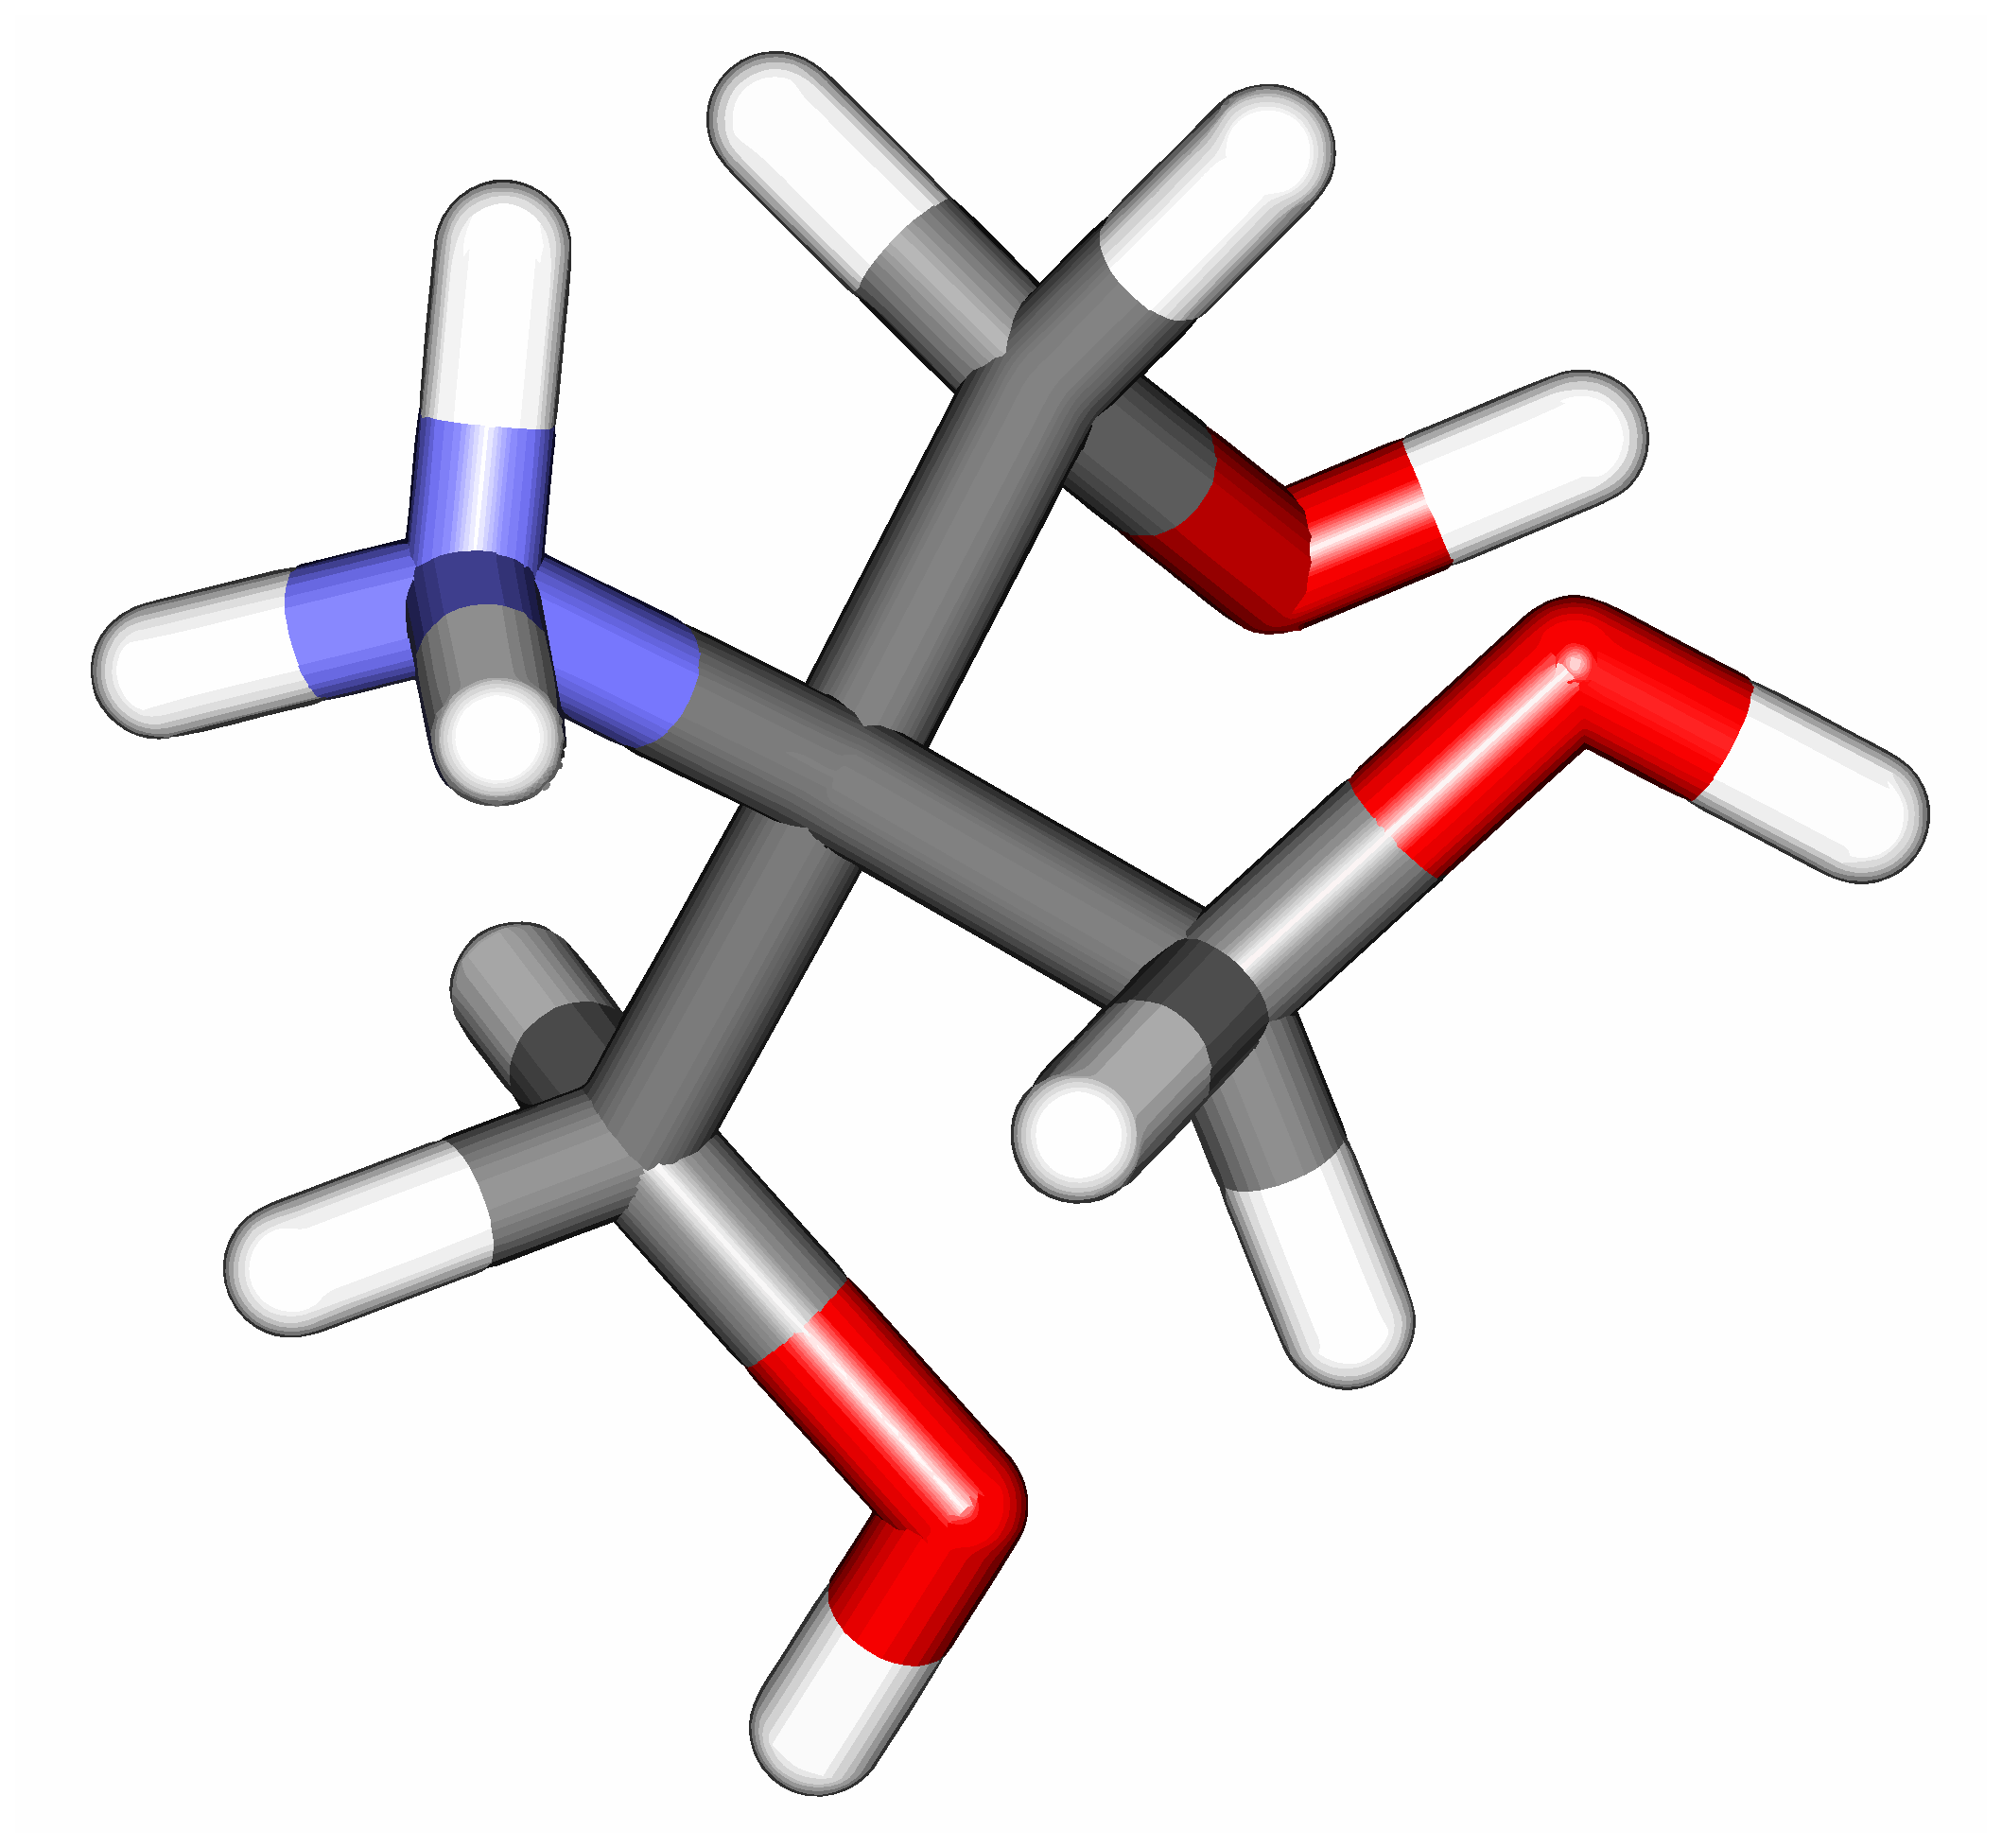
\includegraphics[width=0.10\linewidth]{Figures/Ligands/TRS.eps}
    \label{subfig:Ligands-TRS}
  }
  \subfloat[T27]{
    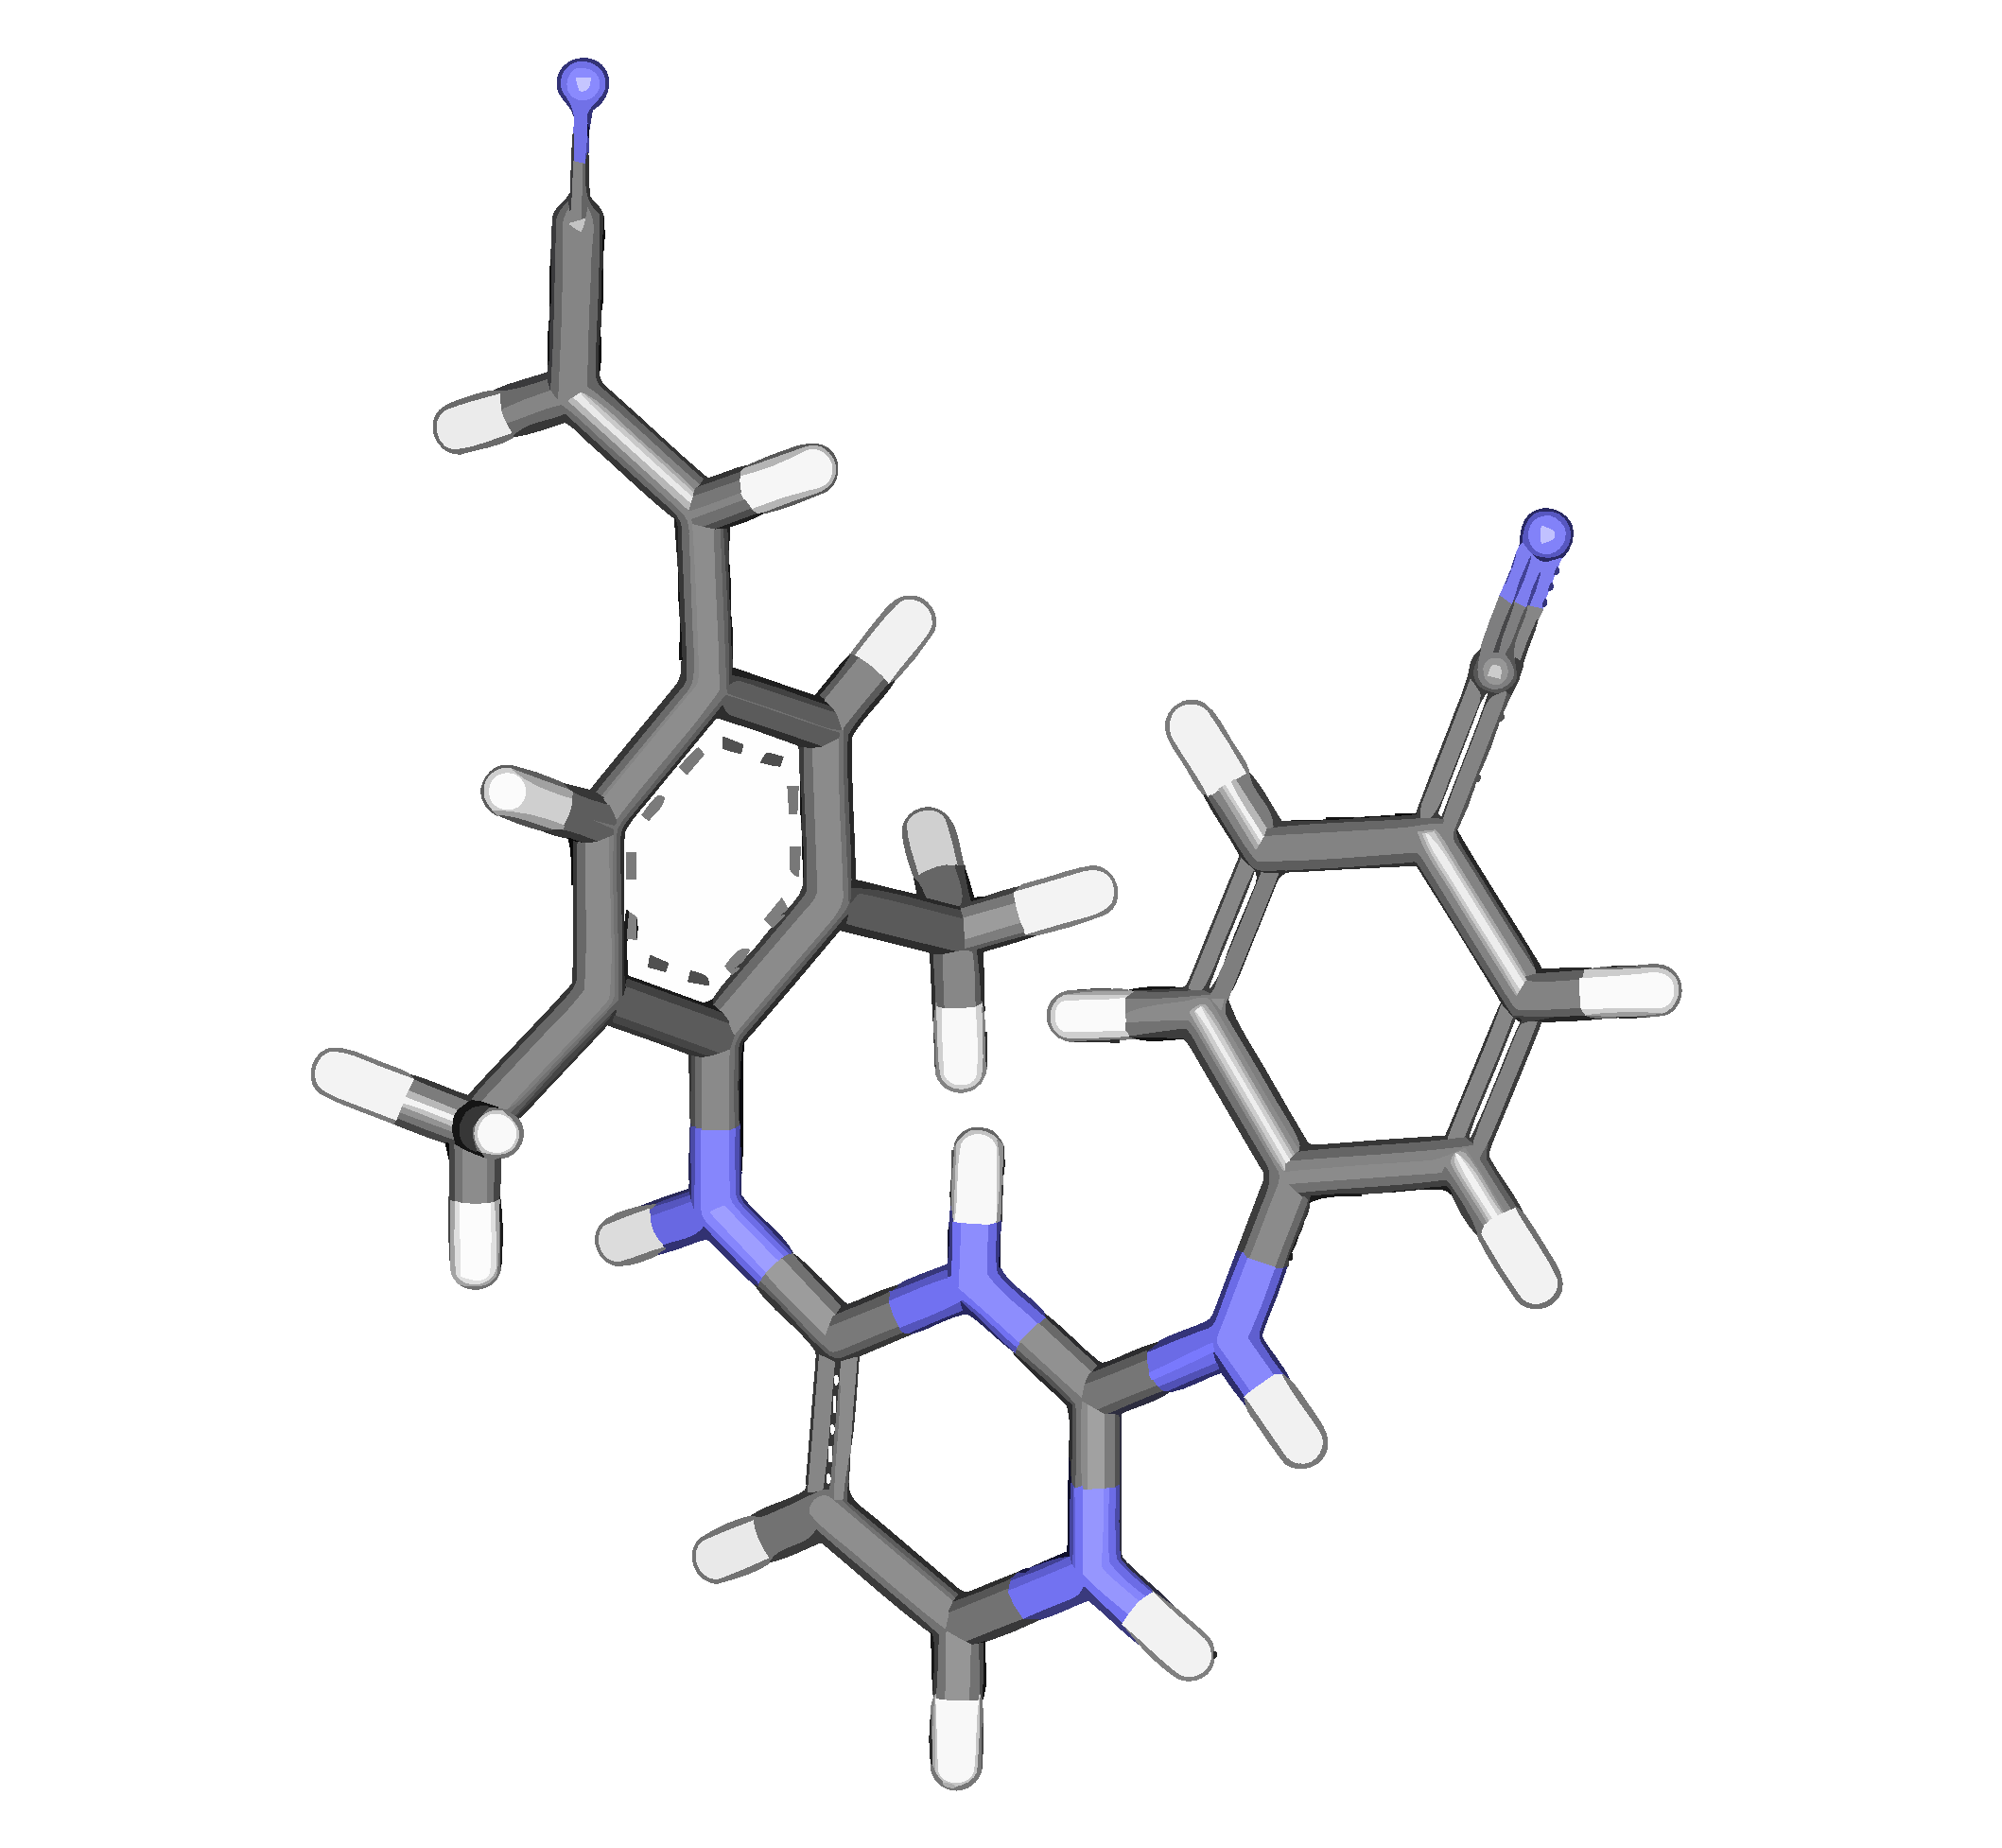
\includegraphics[width=0.10\linewidth]{Figures/Ligands/T27.eps}
    \label{subfig:Ligands-T27}
  }
  \subfloat[4DX]{
    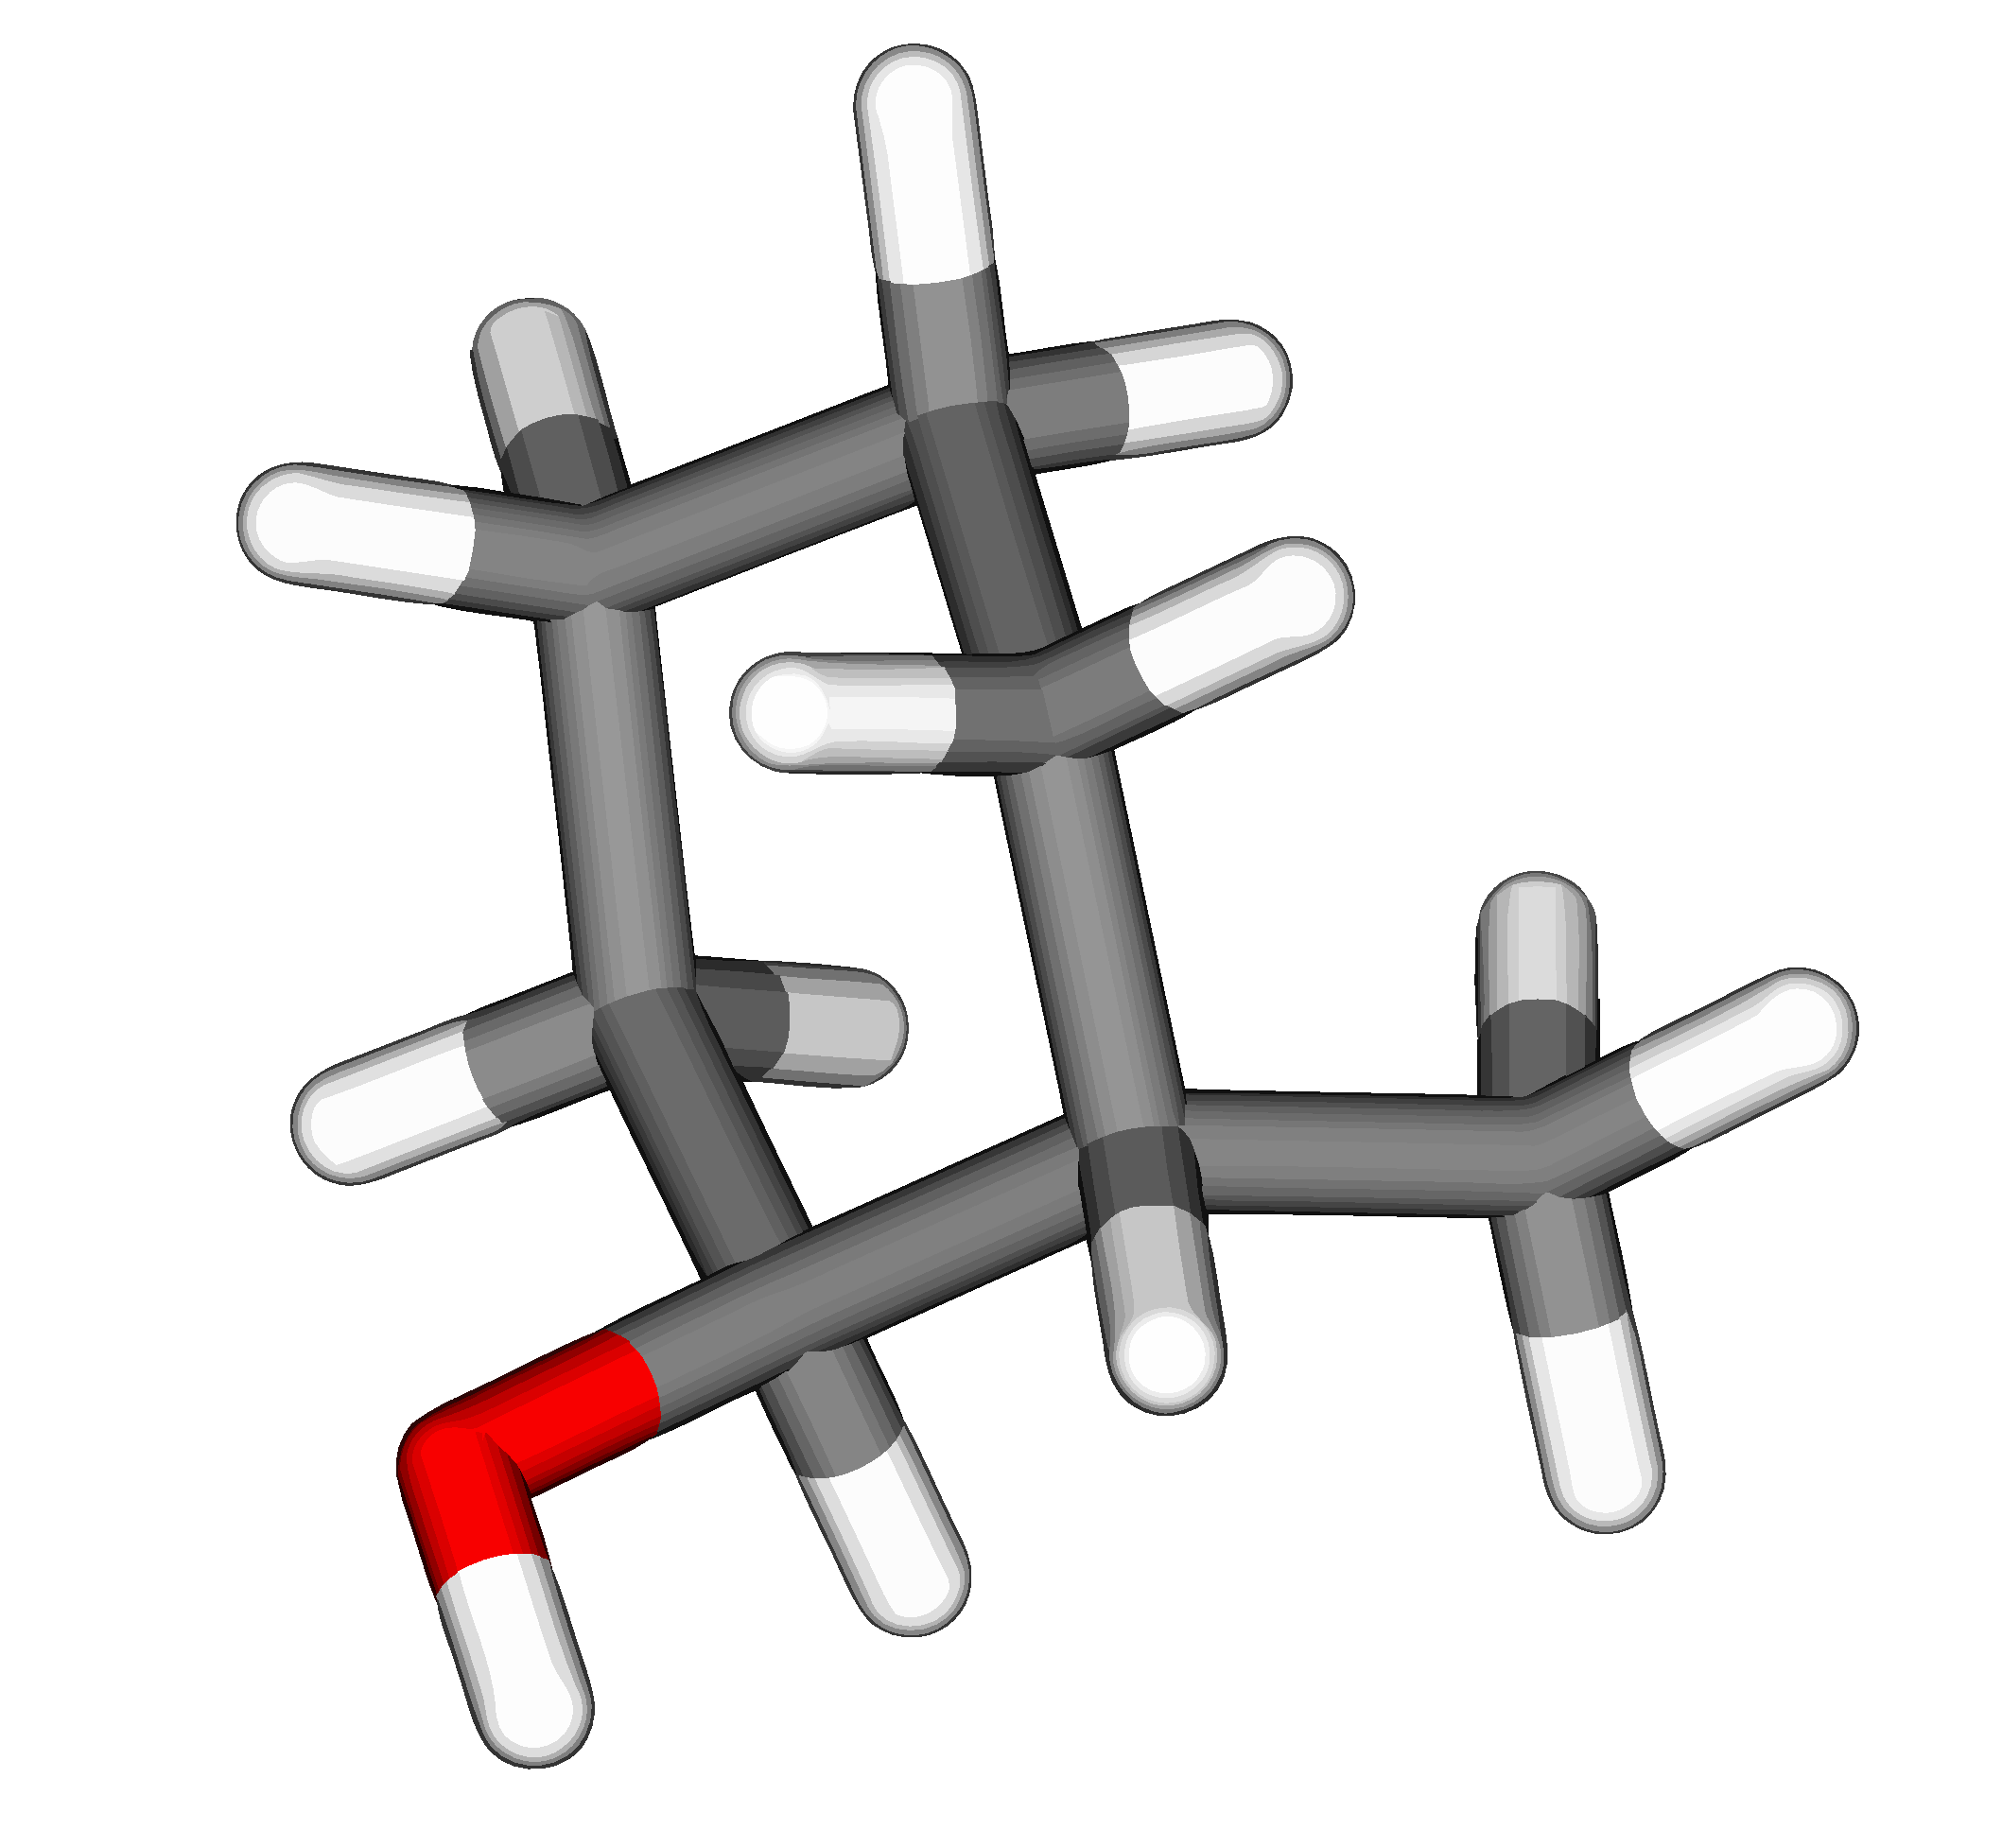
\includegraphics[width=0.10\linewidth]{Figures/Ligands/4DX.eps}
    \label{subfig:Ligands-4DX}
  }
  \subfloat[ZINC01019824]{
    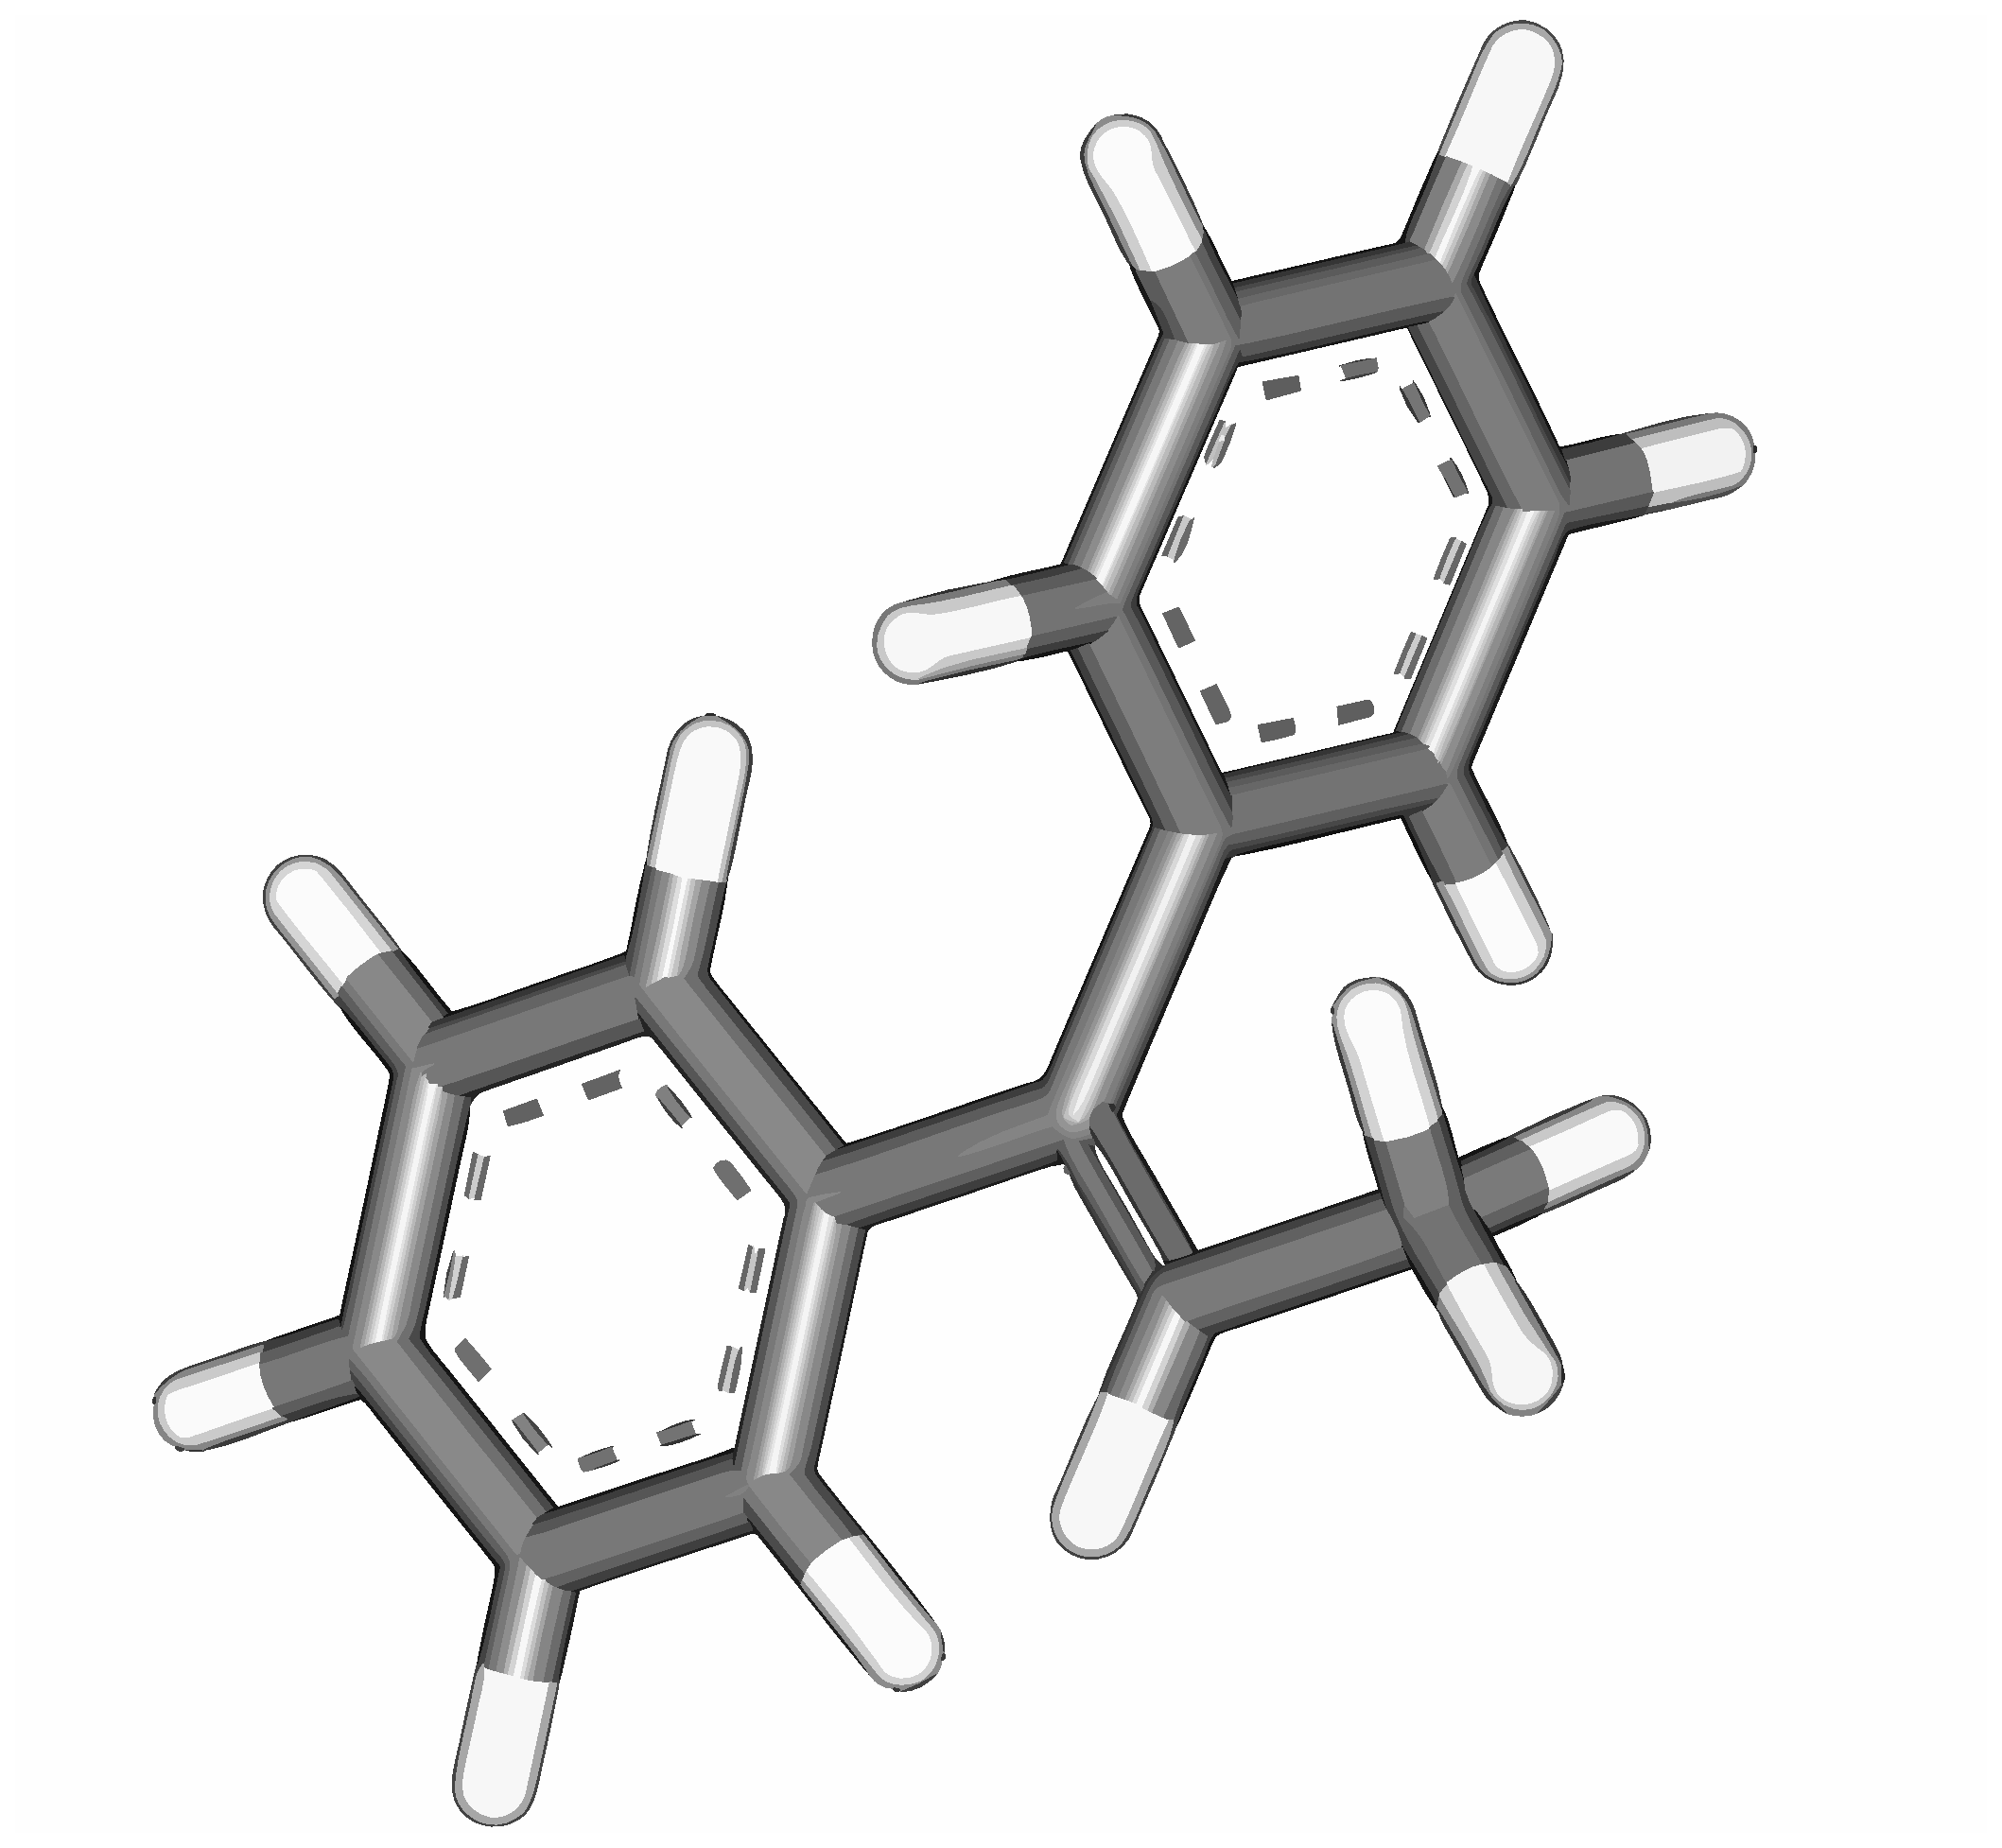
\includegraphics[width=0.10\linewidth]{Figures/Ligands/ZINC01019824.eps}
    \label{subfig:Ligands-ZINC01019824}
  }
  \subfloat[ZINC08442219]{
    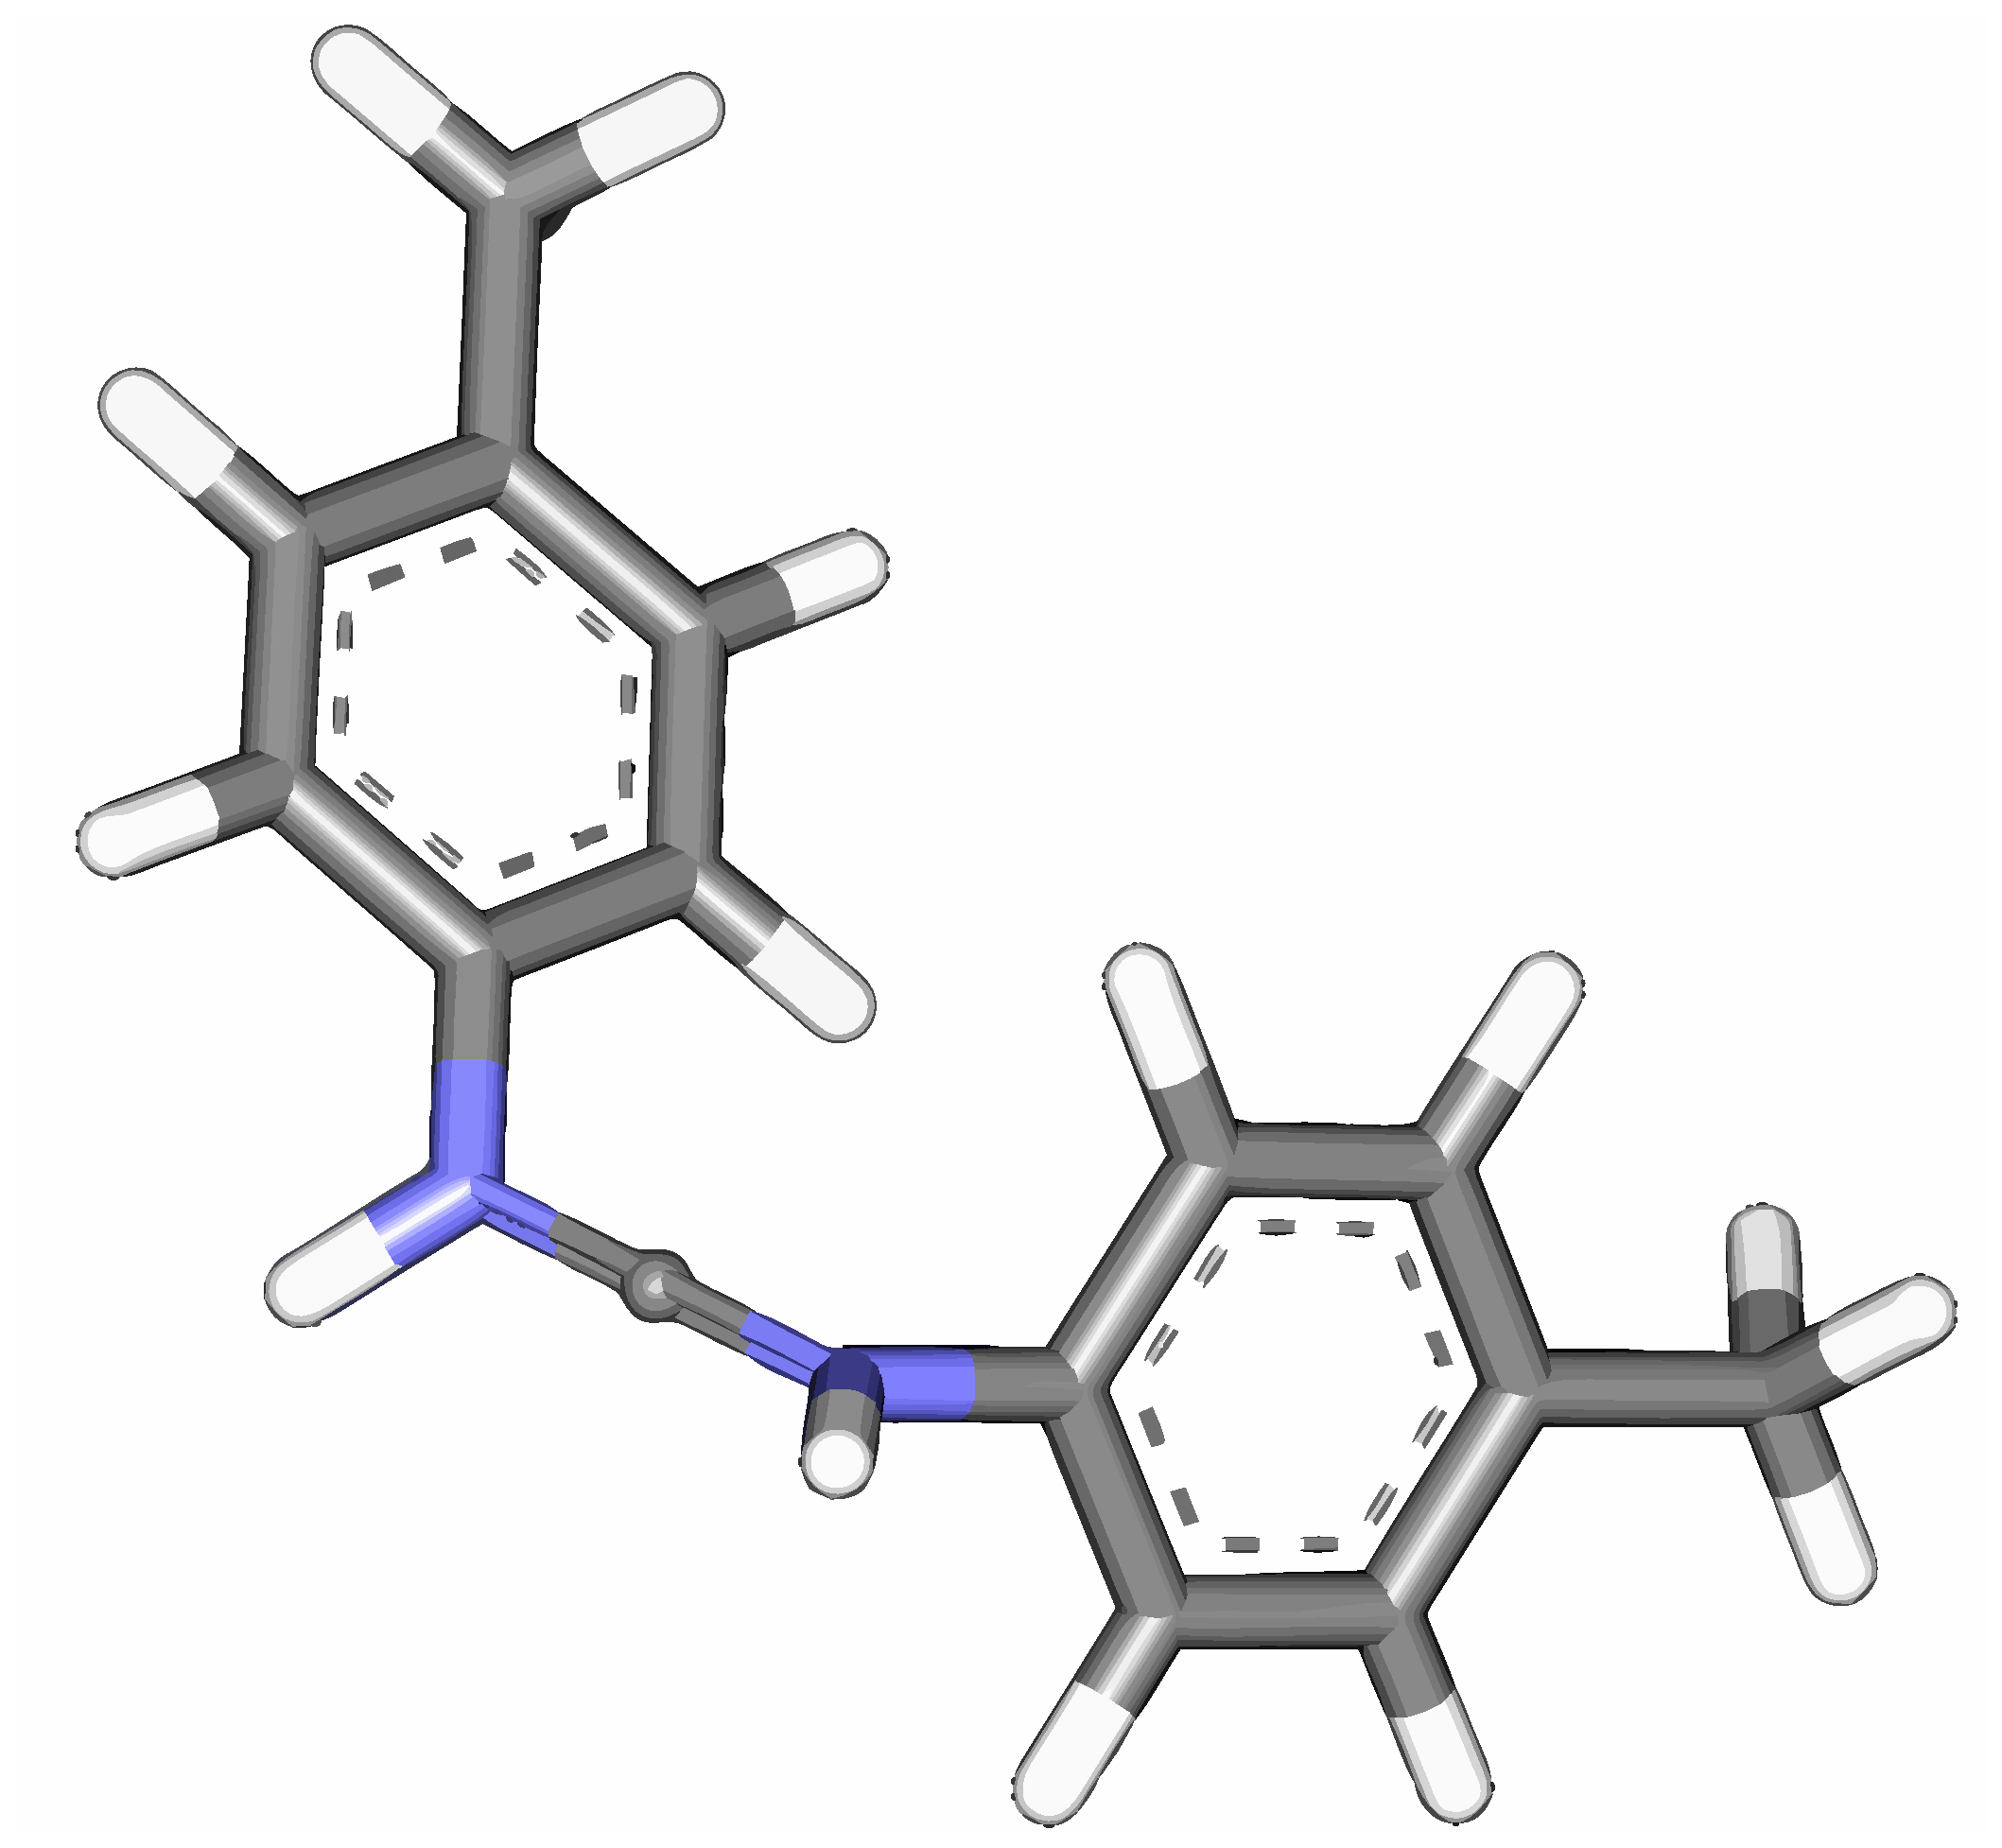
\includegraphics[width=0.10\linewidth]{Figures/Ligands/ZINC08442219.eps}
    \label{subfig:Ligands-ZINC08442219}
  }
  \subfloat[ZINC09365179]{
    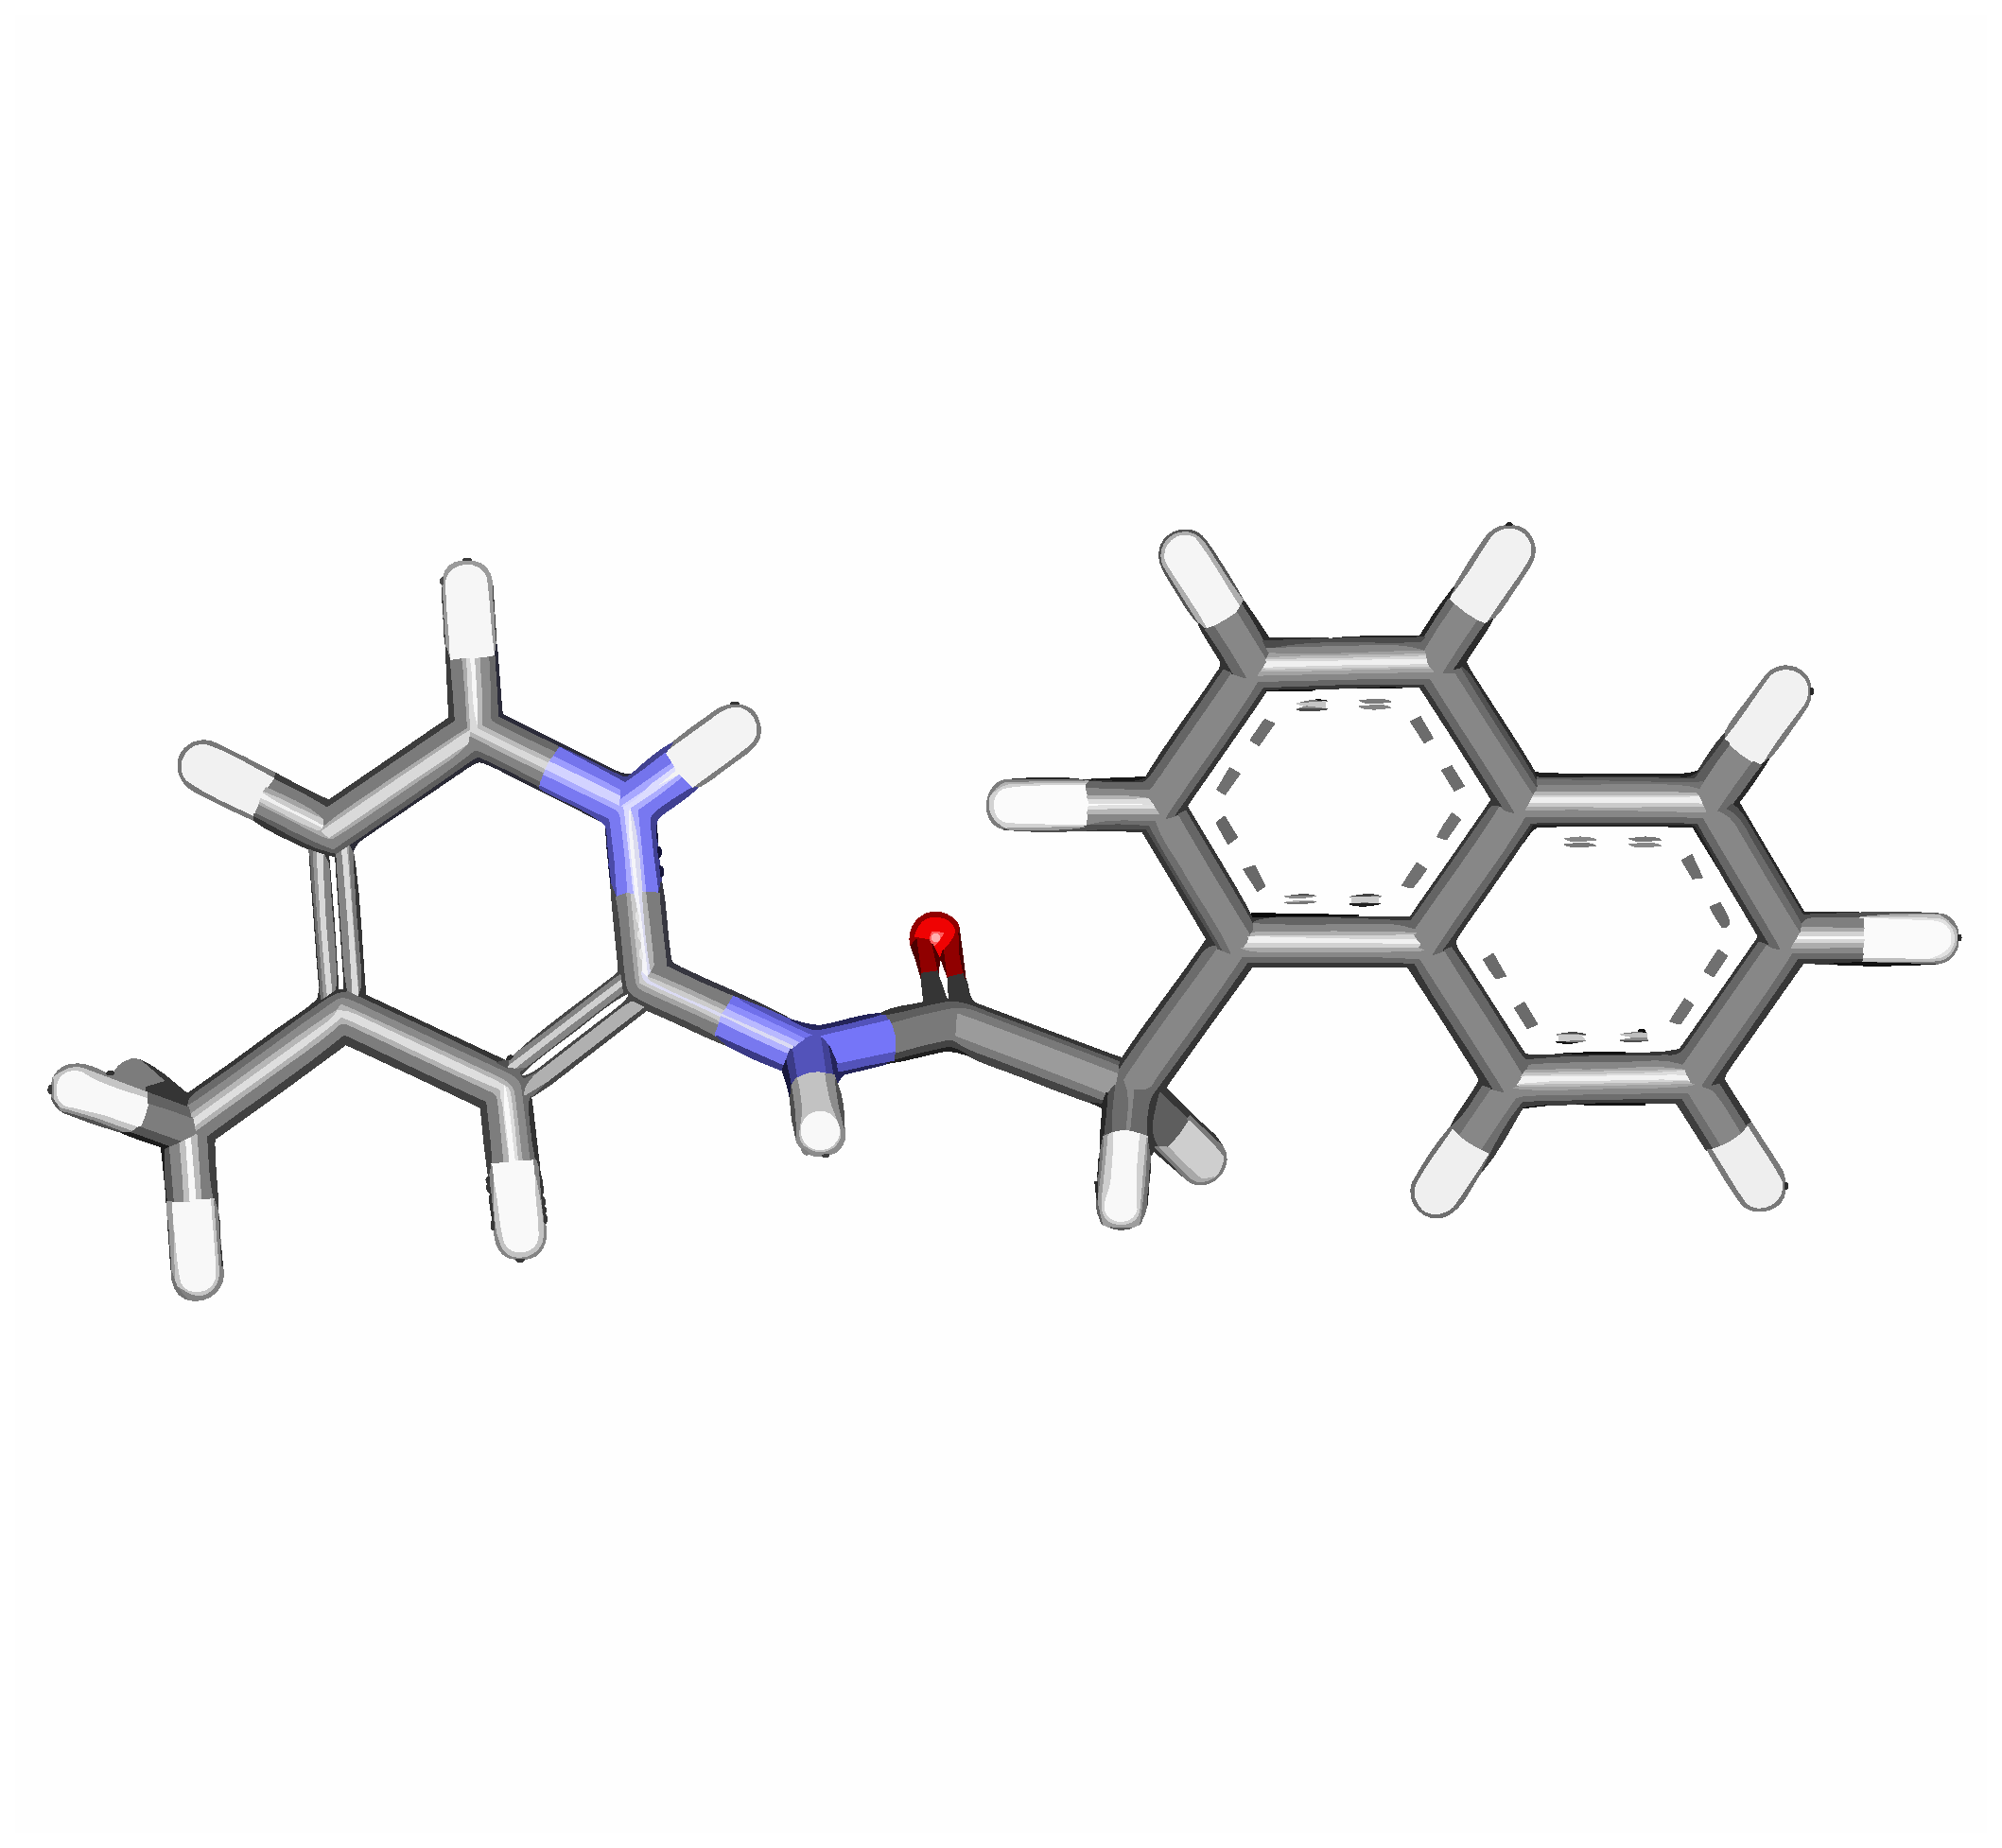
\includegraphics[width=0.10\linewidth]{Figures/Ligands/ZINC09365179.eps}
    \label{subfig:Ligands-ZINC09365179}
  }
  \subfloat[ZINC18153302]{
    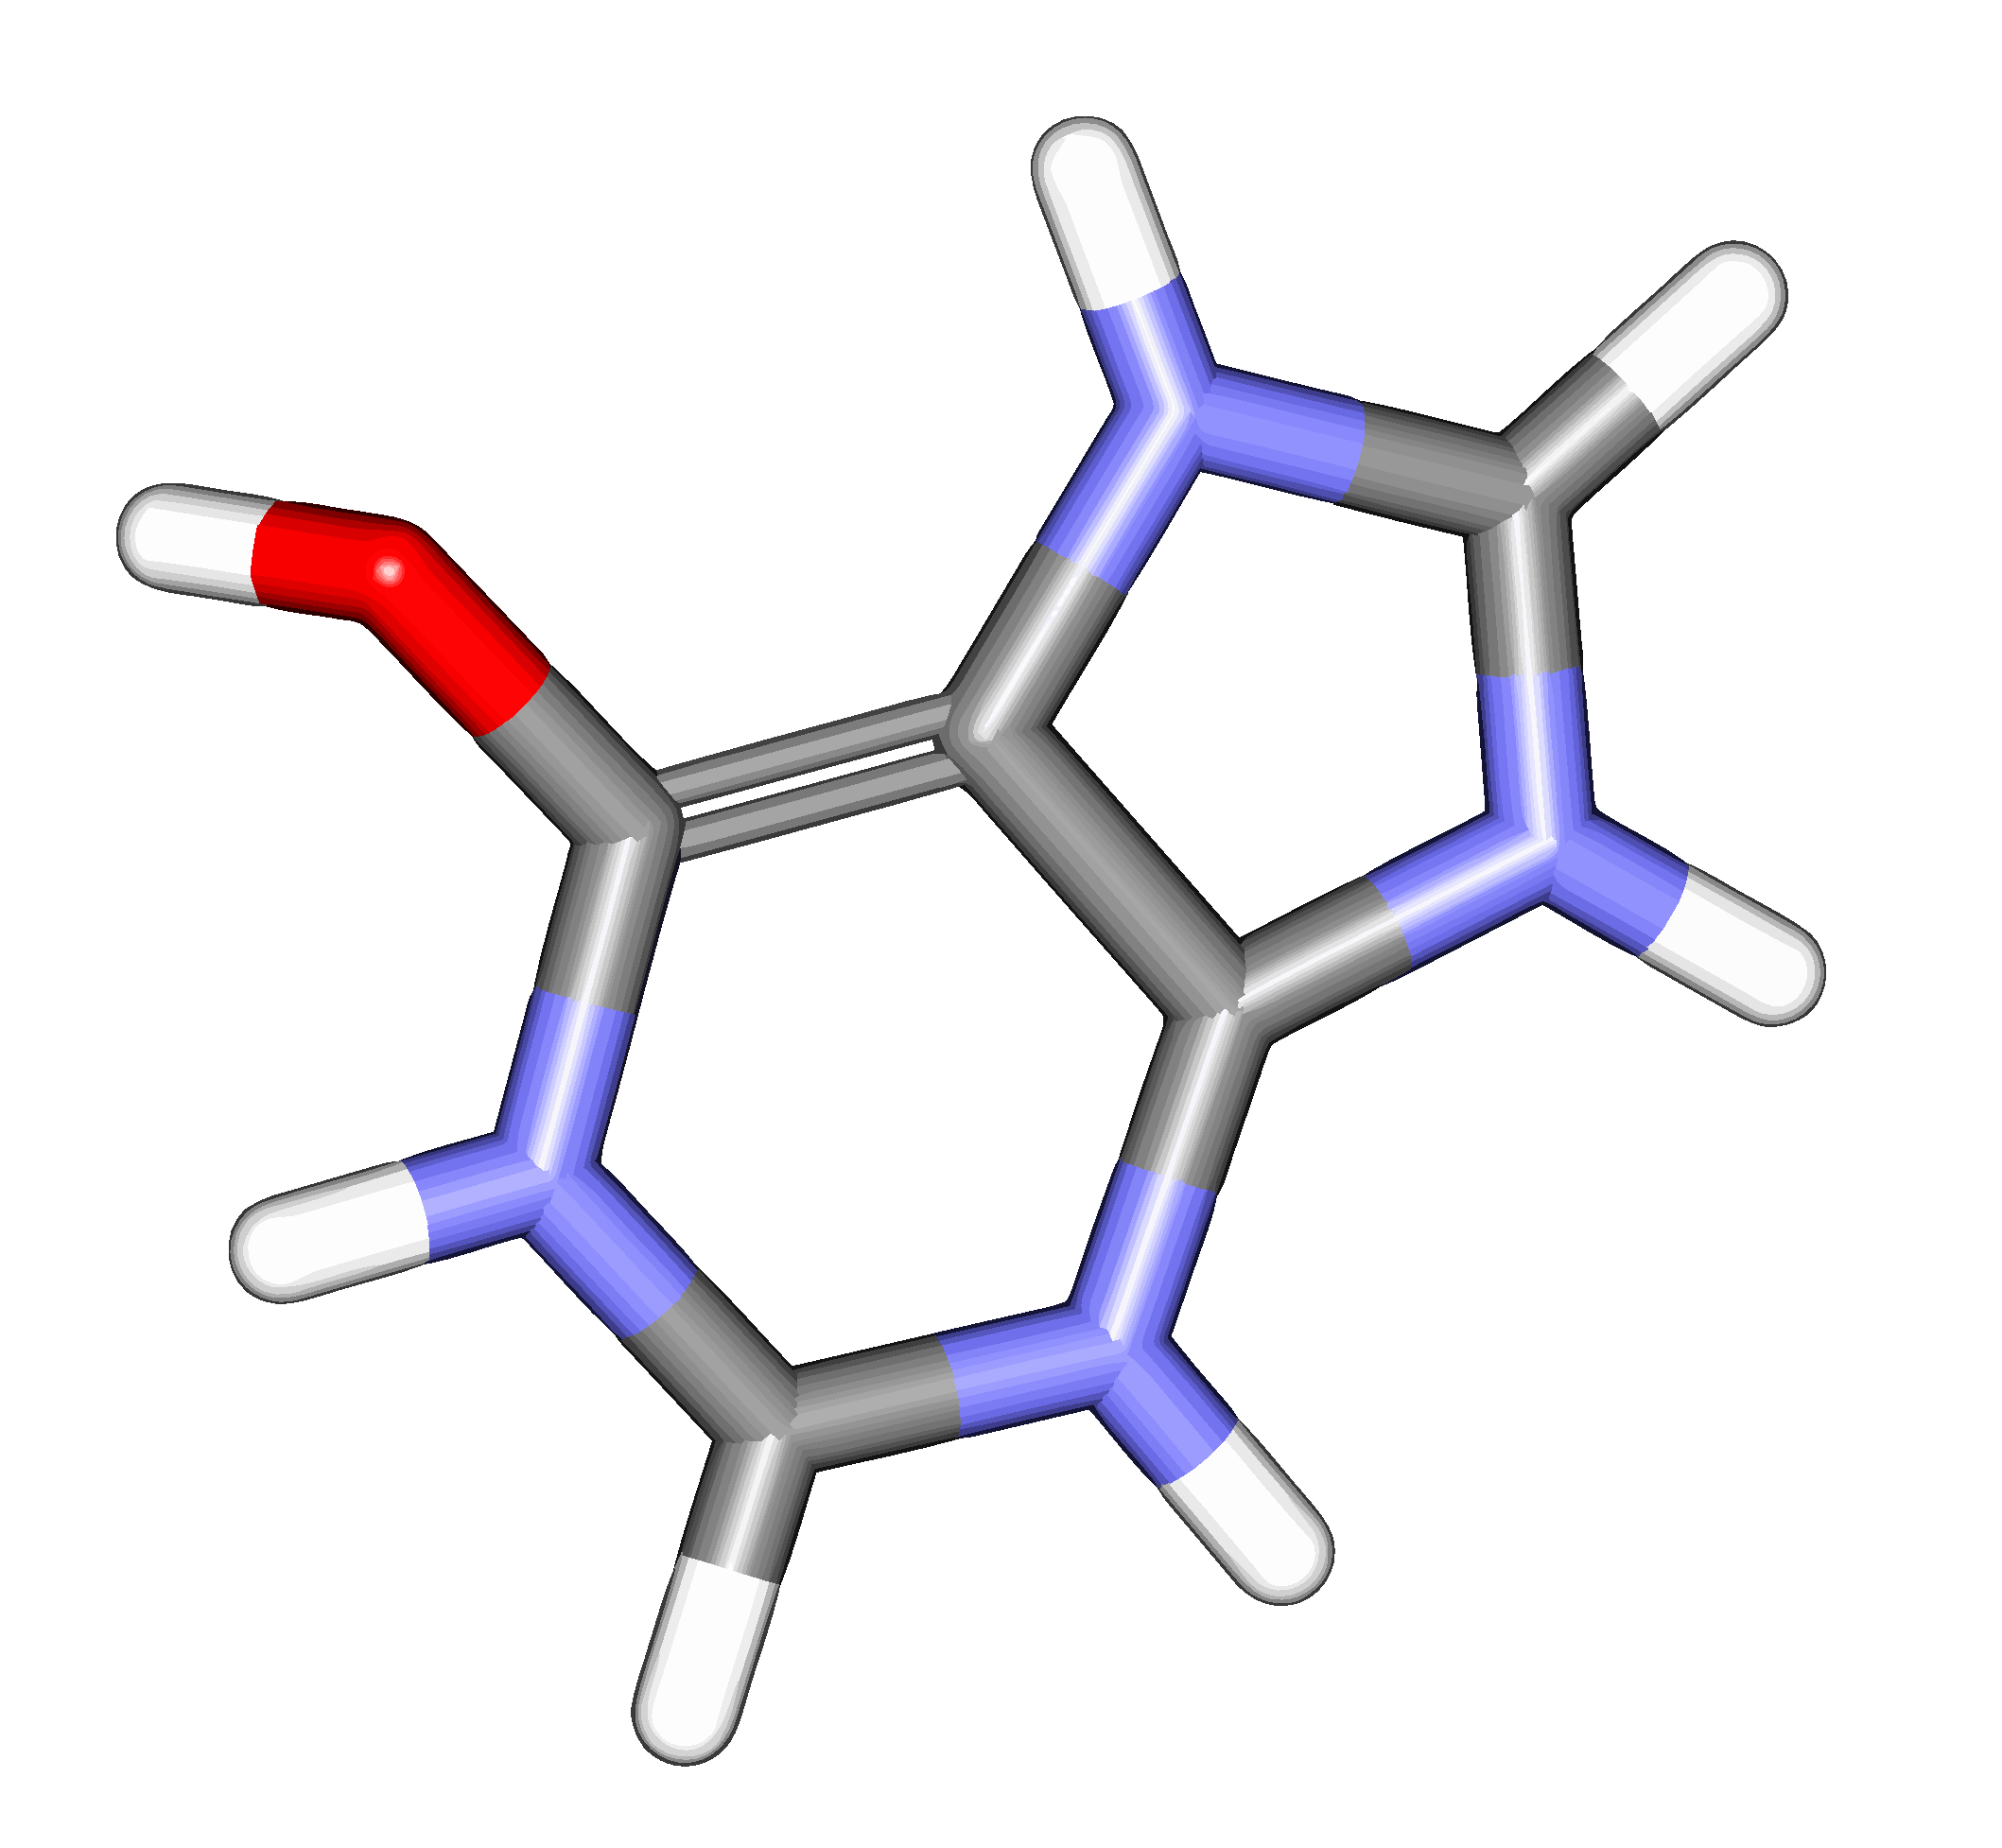
\includegraphics[width=0.10\linewidth]{Figures/Ligands/ZINC18153302.eps}
    \label{subfig:Ligands-ZINC18153302}
  }
  \subfloat[ZINC20030231]{
    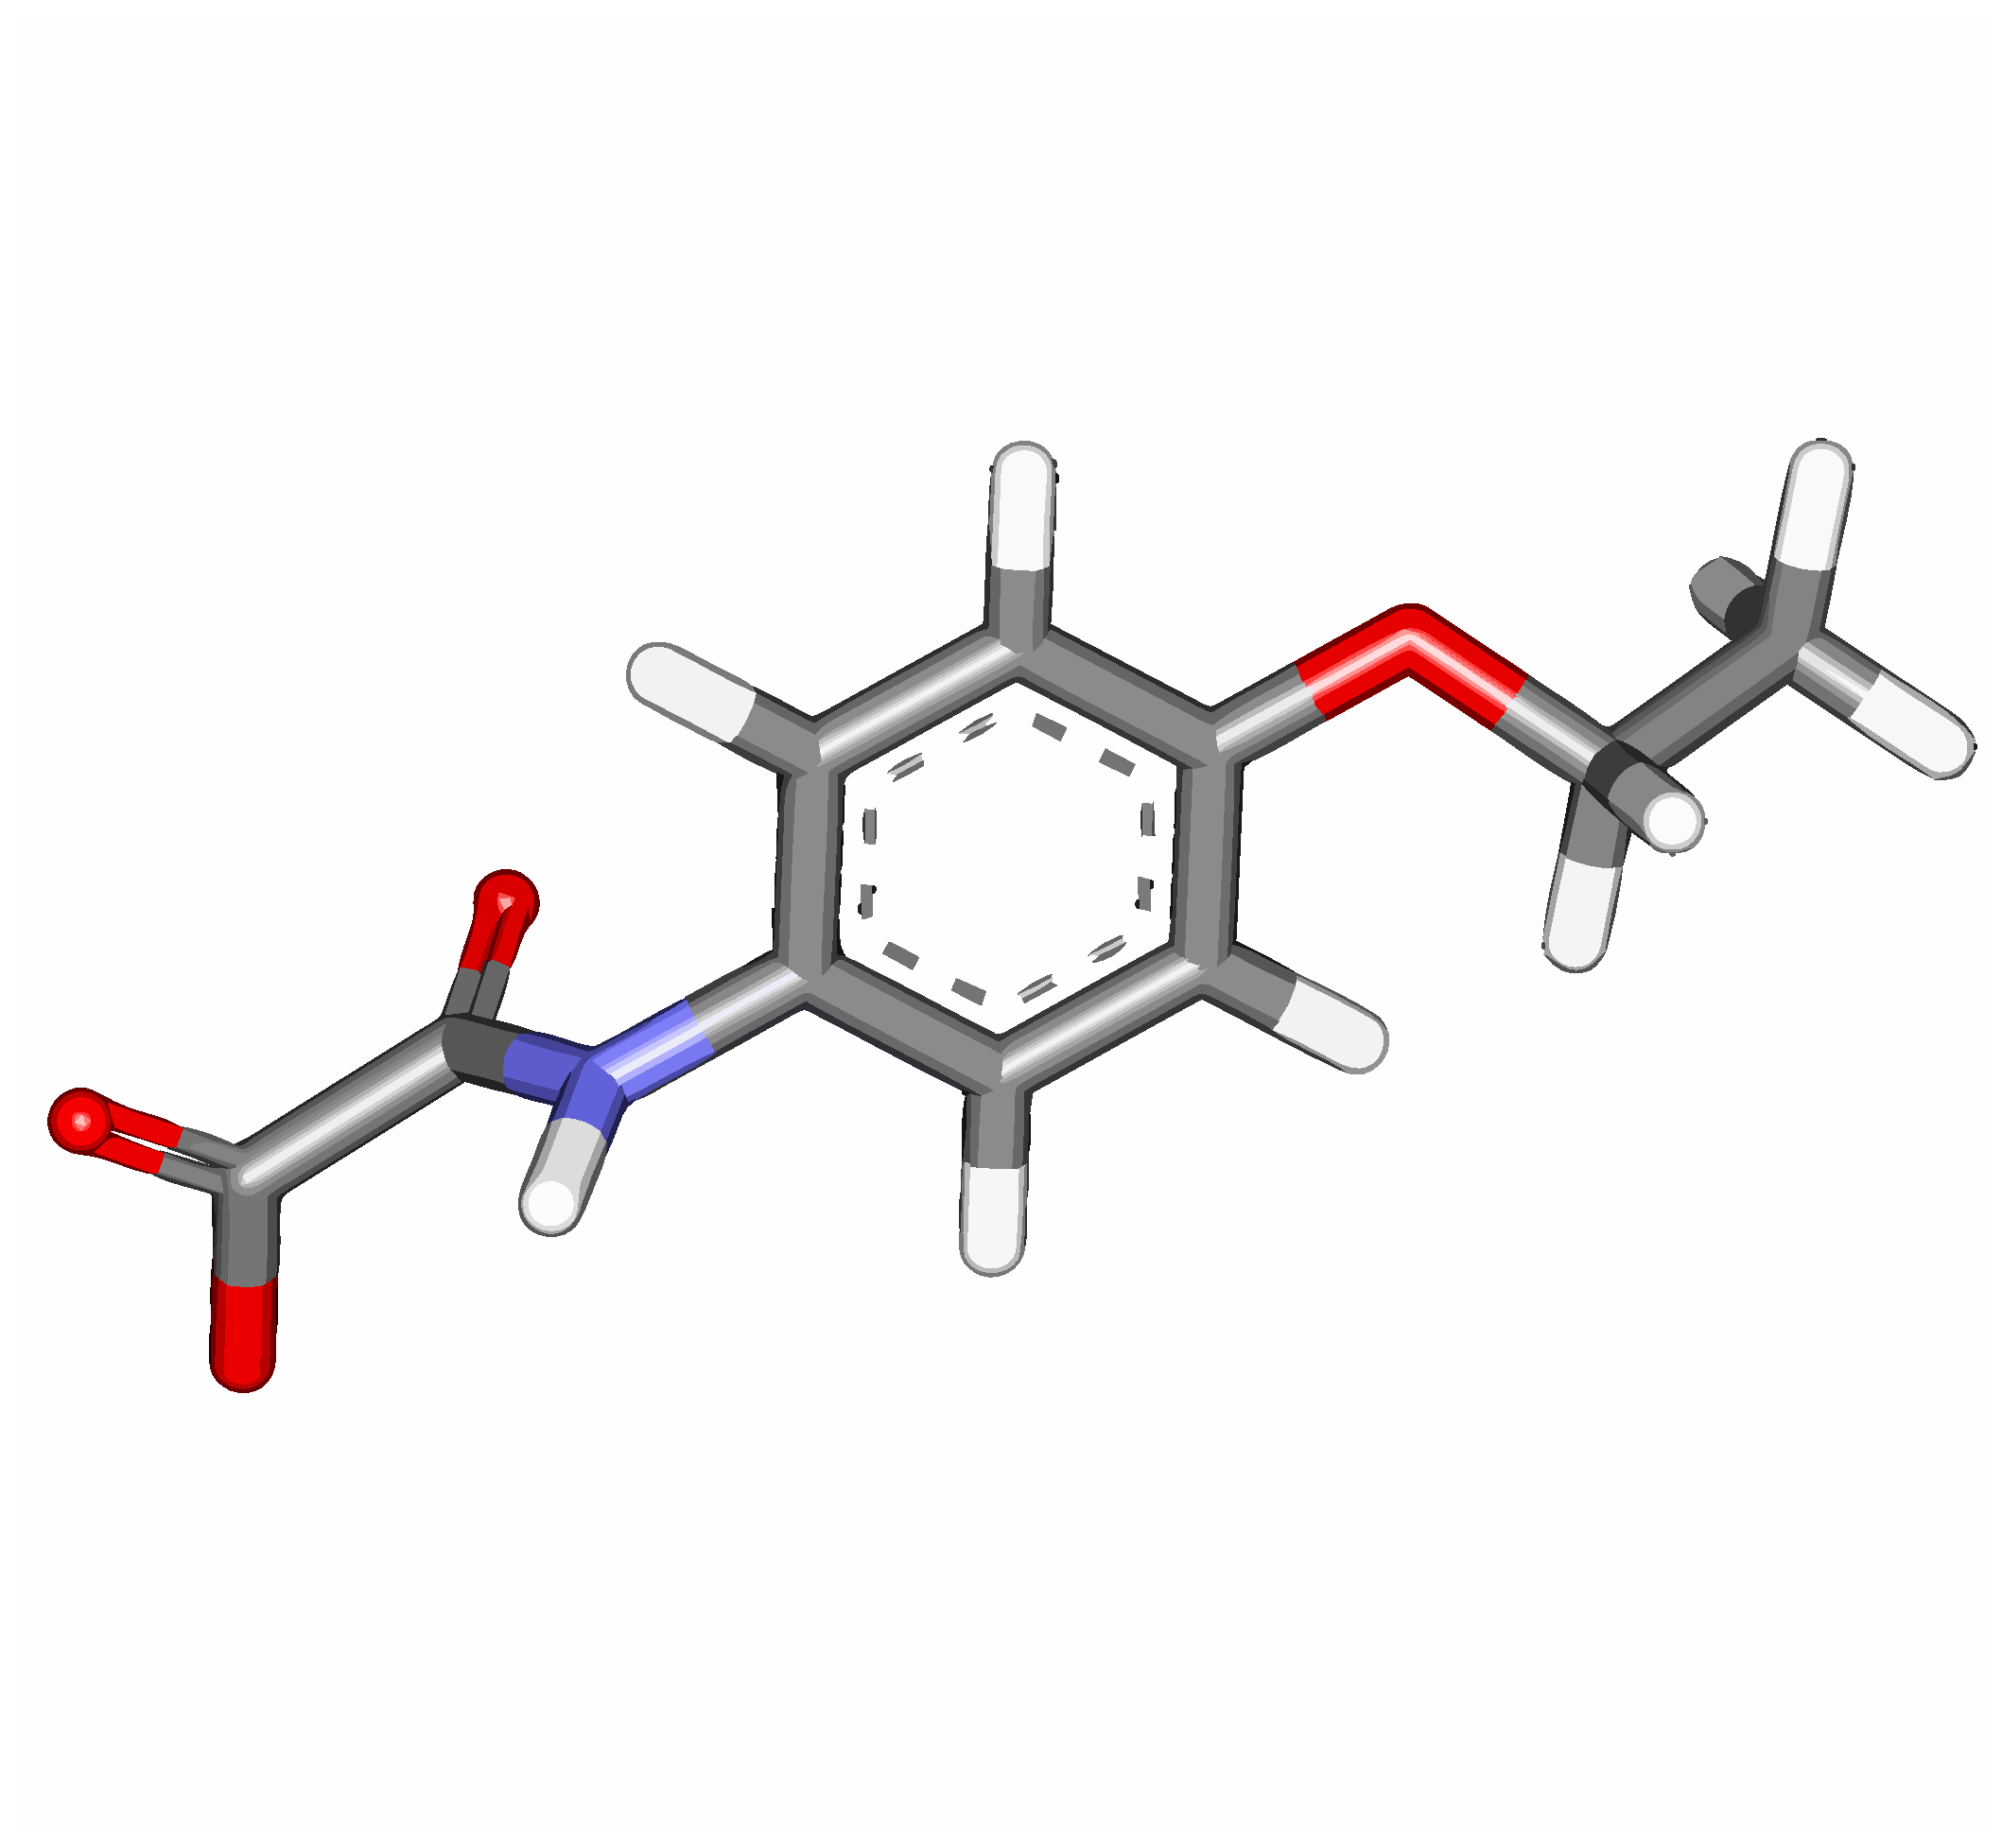
\includegraphics[width=0.10\linewidth]{Figures/Ligands/ZINC20030231.eps}
    \label{subfig:Ligands-ZINC20030231}
  }
  \caption{Stick representations and molecular weights of the 8 unique initial ligands.}
  \label{fig:UniqueInitialLigands}
\end{figure*}

%\begin{table}
%\centering
%\begin{tabular}
%{lr}
%\noalign{\smallskip}\toprule
%Initial Ligand & Predicted Free Energy (kcal/mol)\\
%\midrule
%\noalign{\smallskip}
%\multicolumn{2}{l}{\textbf{Glycogen synthase kinase 3 beta  (1J1B)}} \\
%TRS & -3.8\\
%ZINC01019824 & -6.9\\
%ZINC08442219 & -6.5\\
%ZINC09365179 & -8.3\\
%ZINC18153302 & -4.2\\
%ZINC20030231 & -5.6\\
%\noalign{\smallskip}
%\multicolumn{2}{l}{\textbf{HIV reverse transcriptase (2ZD1)}} \\
%T27 & -13.9\\
%ZINC01019824 & -9.6\\
%ZINC08442219 & -9.1\\
%ZINC09365179 & -11.0\\
%ZINC18153302 & -5.8\\
%ZINC20030231 & -7.1\\
%\noalign{\smallskip}
%\multicolumn{2}{l}{\textbf{HIV protease (3KFN)}} \\
%4DX & -4.0\\
%ZINC01019824 & -5.9\\
%ZINC08442219 & -5.6\\
%ZINC09365179 & -6.4\\
%ZINC18153302 & -4.1\\
%ZINC20030231 & -4.9\\
%\bottomrule
%\end{tabular}
%\caption{Free energies of the 18 initial ligands categorized by 3 receptors.}
%\label{tab:InitialLigands}
%\end{table}

Phosphorus is a very common chemical element found in drugs. However, AutoGrow does not natively support phosphorus. Its bond length library does not include phosphorus, so it must rely on PDB CONECT records to detect covalent bonds. In contrast, igrow has built-in support for phosphorus. Its source code incorporates bond lengths for phosphorus, so it can recover covalent bonds from PDB ATOM/HETATM records. To test such capability, we picked an additional phosphorus-containing ligand named TFO from PDB, and generated ligands from TFO docking to HIV reverse transcriptase. The input ligand file consists of ATOM records only.

\subsection{Fragment Library}
Ligands are mutated by appending new fragments from a fragment library.
There are two fragment libraries that accompanied with the release of AutoGrow, namely the small-fragment and the large-fragment libraries.
We tested both libraries internally, and noticed early convergence when using the large-fragment library, which was quite problematic for testing purposes.
So we focused on the small-fragment library, which is made up of 46 fragments.
They are small in size, having 3 to 15 atoms and an average of 9.6 atoms with a standard deviation of 2.8 \cite{114}.

\section{Results}\label{sec:results}
We tested igrow v1.14 and compared it with AutoGrow 2.0.4, the most recent versions of both programs at the moment this paper was composed.
The parameter settings for AutoGrow and igrow are listed in table \ref{tab:ParameterSettings}.
The default values for AutoGrow were retained, i.e. 10, 20, 20, and 8 for the number of elitists, children, mutants, and generations, respectively.
Docking frequency refers to the frequency that the individual candidates of the population will be evaluated by docking. In AutoGrow, this value is fixed to 1 because population evaluation is always done by docking for each generation. Since igrow supports population evaluation by either docking or scoring only, its docking frequency was set to 3 to examine this special feature. In this case, evaluation by docking occurs every 3 generations, i.e. evaluation in generations 3, 6, 9, etc. is done by docking, and evaluation in generations 1, 2, 4, 5, 7, 8, etc. is done by scoring only. In order to retain a same number of evaluations by docking, the number of generations for igrow was thus set to 24 instead of 8 in the case of AutoGrow.
The maximum number of atoms was set to 80 because we noticed from initial trials that the generated ligands of final generation consisted of around 70 atoms but their molecular weight already exceeded 500 Da.
To make a fair comparison, the settings for igrow were set to be identical to AutoGrow except for the number of generations and docking frequency.

\begin{table}
\centering
\begin{tabular}
{lrr}
\noalign{\smallskip}\toprule
Program & AutoGrow & igrow\\
\midrule
\noalign{\smallskip}
Number of elitists & 10 & 10\\
Number of children & 20 & 20\\
Number of mutants & 20 & 20\\
Number of generations & 8 & 24\\
Docking frequency & 1 & 3\\
Max number of atoms & 80 & 80\\
\bottomrule
\end{tabular}
\caption{Parameter settings for AutoGrow and igrow. Elitists refer to the best ligands of a generation that will survive directly into the next generation. Children refer to ligands generated by crossover. Mutants refer to ligands generated by mutation.}
\label{tab:ParameterSettings}
\end{table}

So far we have collected 3 receptors, each of which is associated with 6 initial ligands. Therefore there are 18 test cases in total.
Since genetic algorithm is stochastic, we ran AutoGrow and igrow for 9 times for each test case under the parameter settings shown in \ref{tab:ParameterSettings}, simultaneously on 6 Linux machines with Ubuntu 10.04.1 x86\_64, Dual Intel Xeon Quad Core 2.4GHz, and 32GB RAM.
Each AutoGrow execution and igrow execution cost approximately 3 hours and 2.4 hours respectively on average.

\subsection{Binding Pose}
In order to validate the correctness of ligands generated by igrow, we picked out the best ligand from each test case and visualized it in complex of its corresponding receptor.
Here, the best ligand refers to the one that have the lowest free energy.
Figure \ref{fig:BestLigands} demonstrates one particular test case.
(more test cases are given in the supplementary materials)

\begin{figure*}[p]
  \centering
  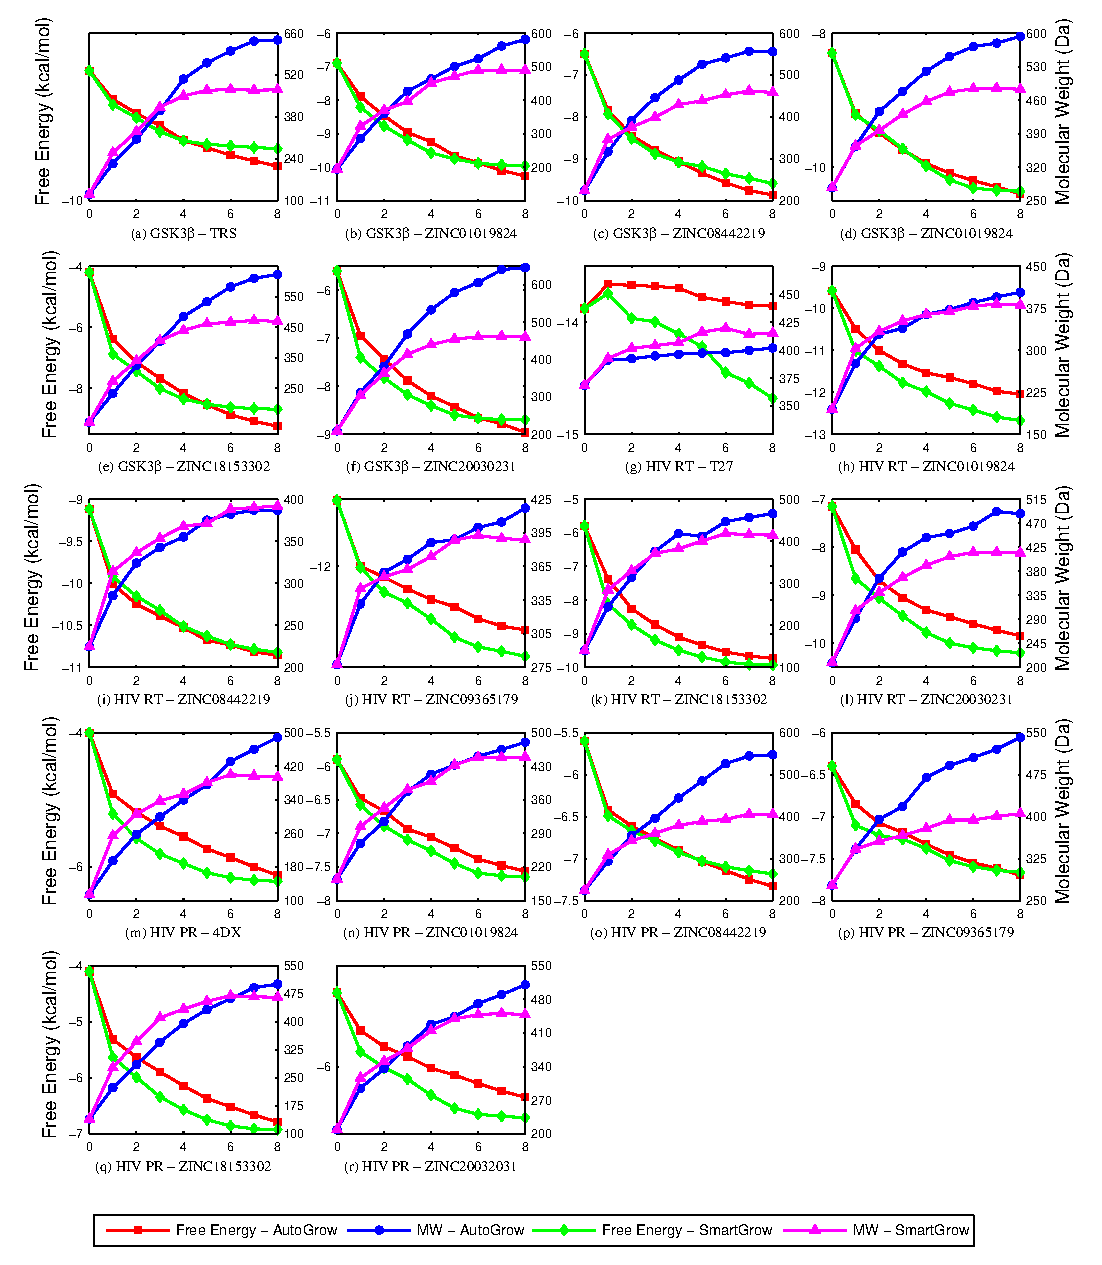
\includegraphics[width=1\linewidth]{Figures/Results/Best5.eps}
  \caption{Average free energies and molecular weights of the best 5 ligands generated by AutoGrow and igrow of each generation. Generation 0 refers to the initial ligand. Blue circles: average free energies of the best 5 ligands generated by AutoGrow. Green diamonds: average free energies of the best 5 ligands generated by igrow. Red squares: average molecular weights of the best 5 ligands generated by AutoGrow. Purple triangles: average molecular weights of the best 5 ligands generated by igrow. First 6 initial ligands dock to glycogen synthase kinase 3 beta. Middle 6 initial ligands dock to HIV reverse transcriptase. Last 6 initial ligands dock to HIV protease.}
  \label{fig:Best5}
\end{figure*}

\begin{figure*}
  \centering
  \subfloat[Initial ligand.]{
    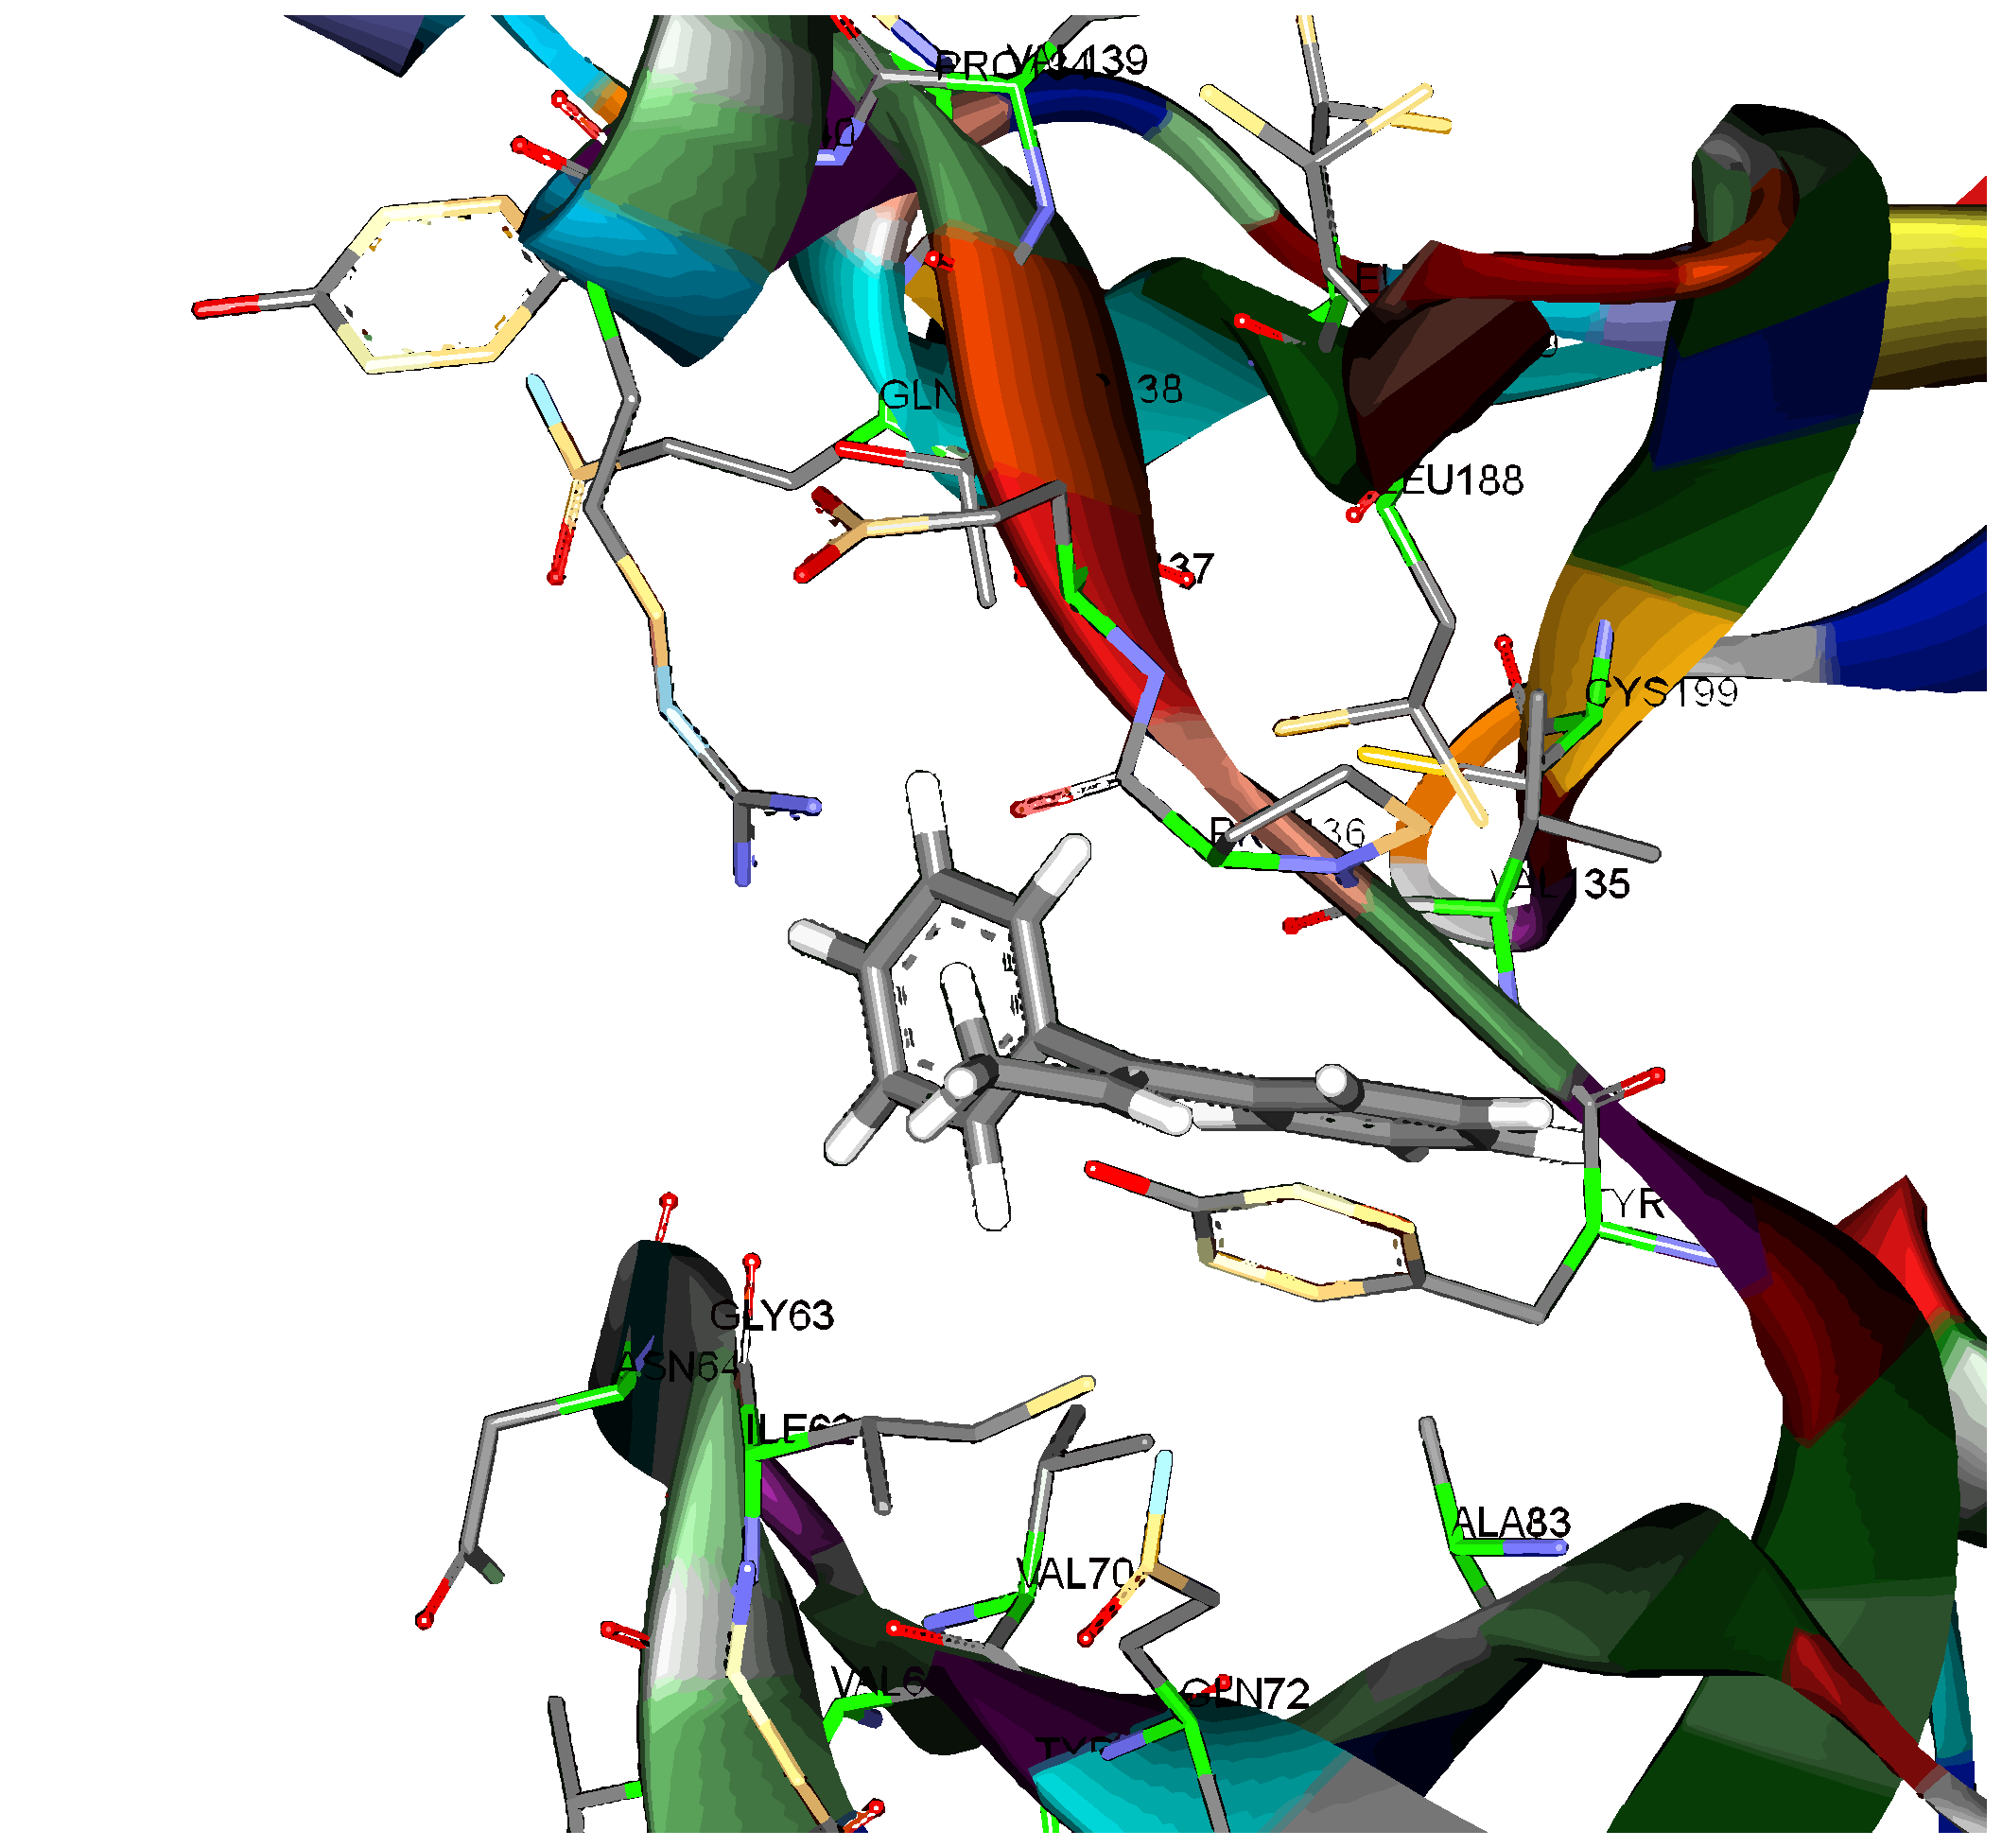
\includegraphics[width=0.31\linewidth]{Figures/Results/1J1B-ZINC01019824.eps}
    \label{subfig:1J1B-ZINC01019824}
  }
  \subfloat[The best ligand generated by AutoGrow.]{
    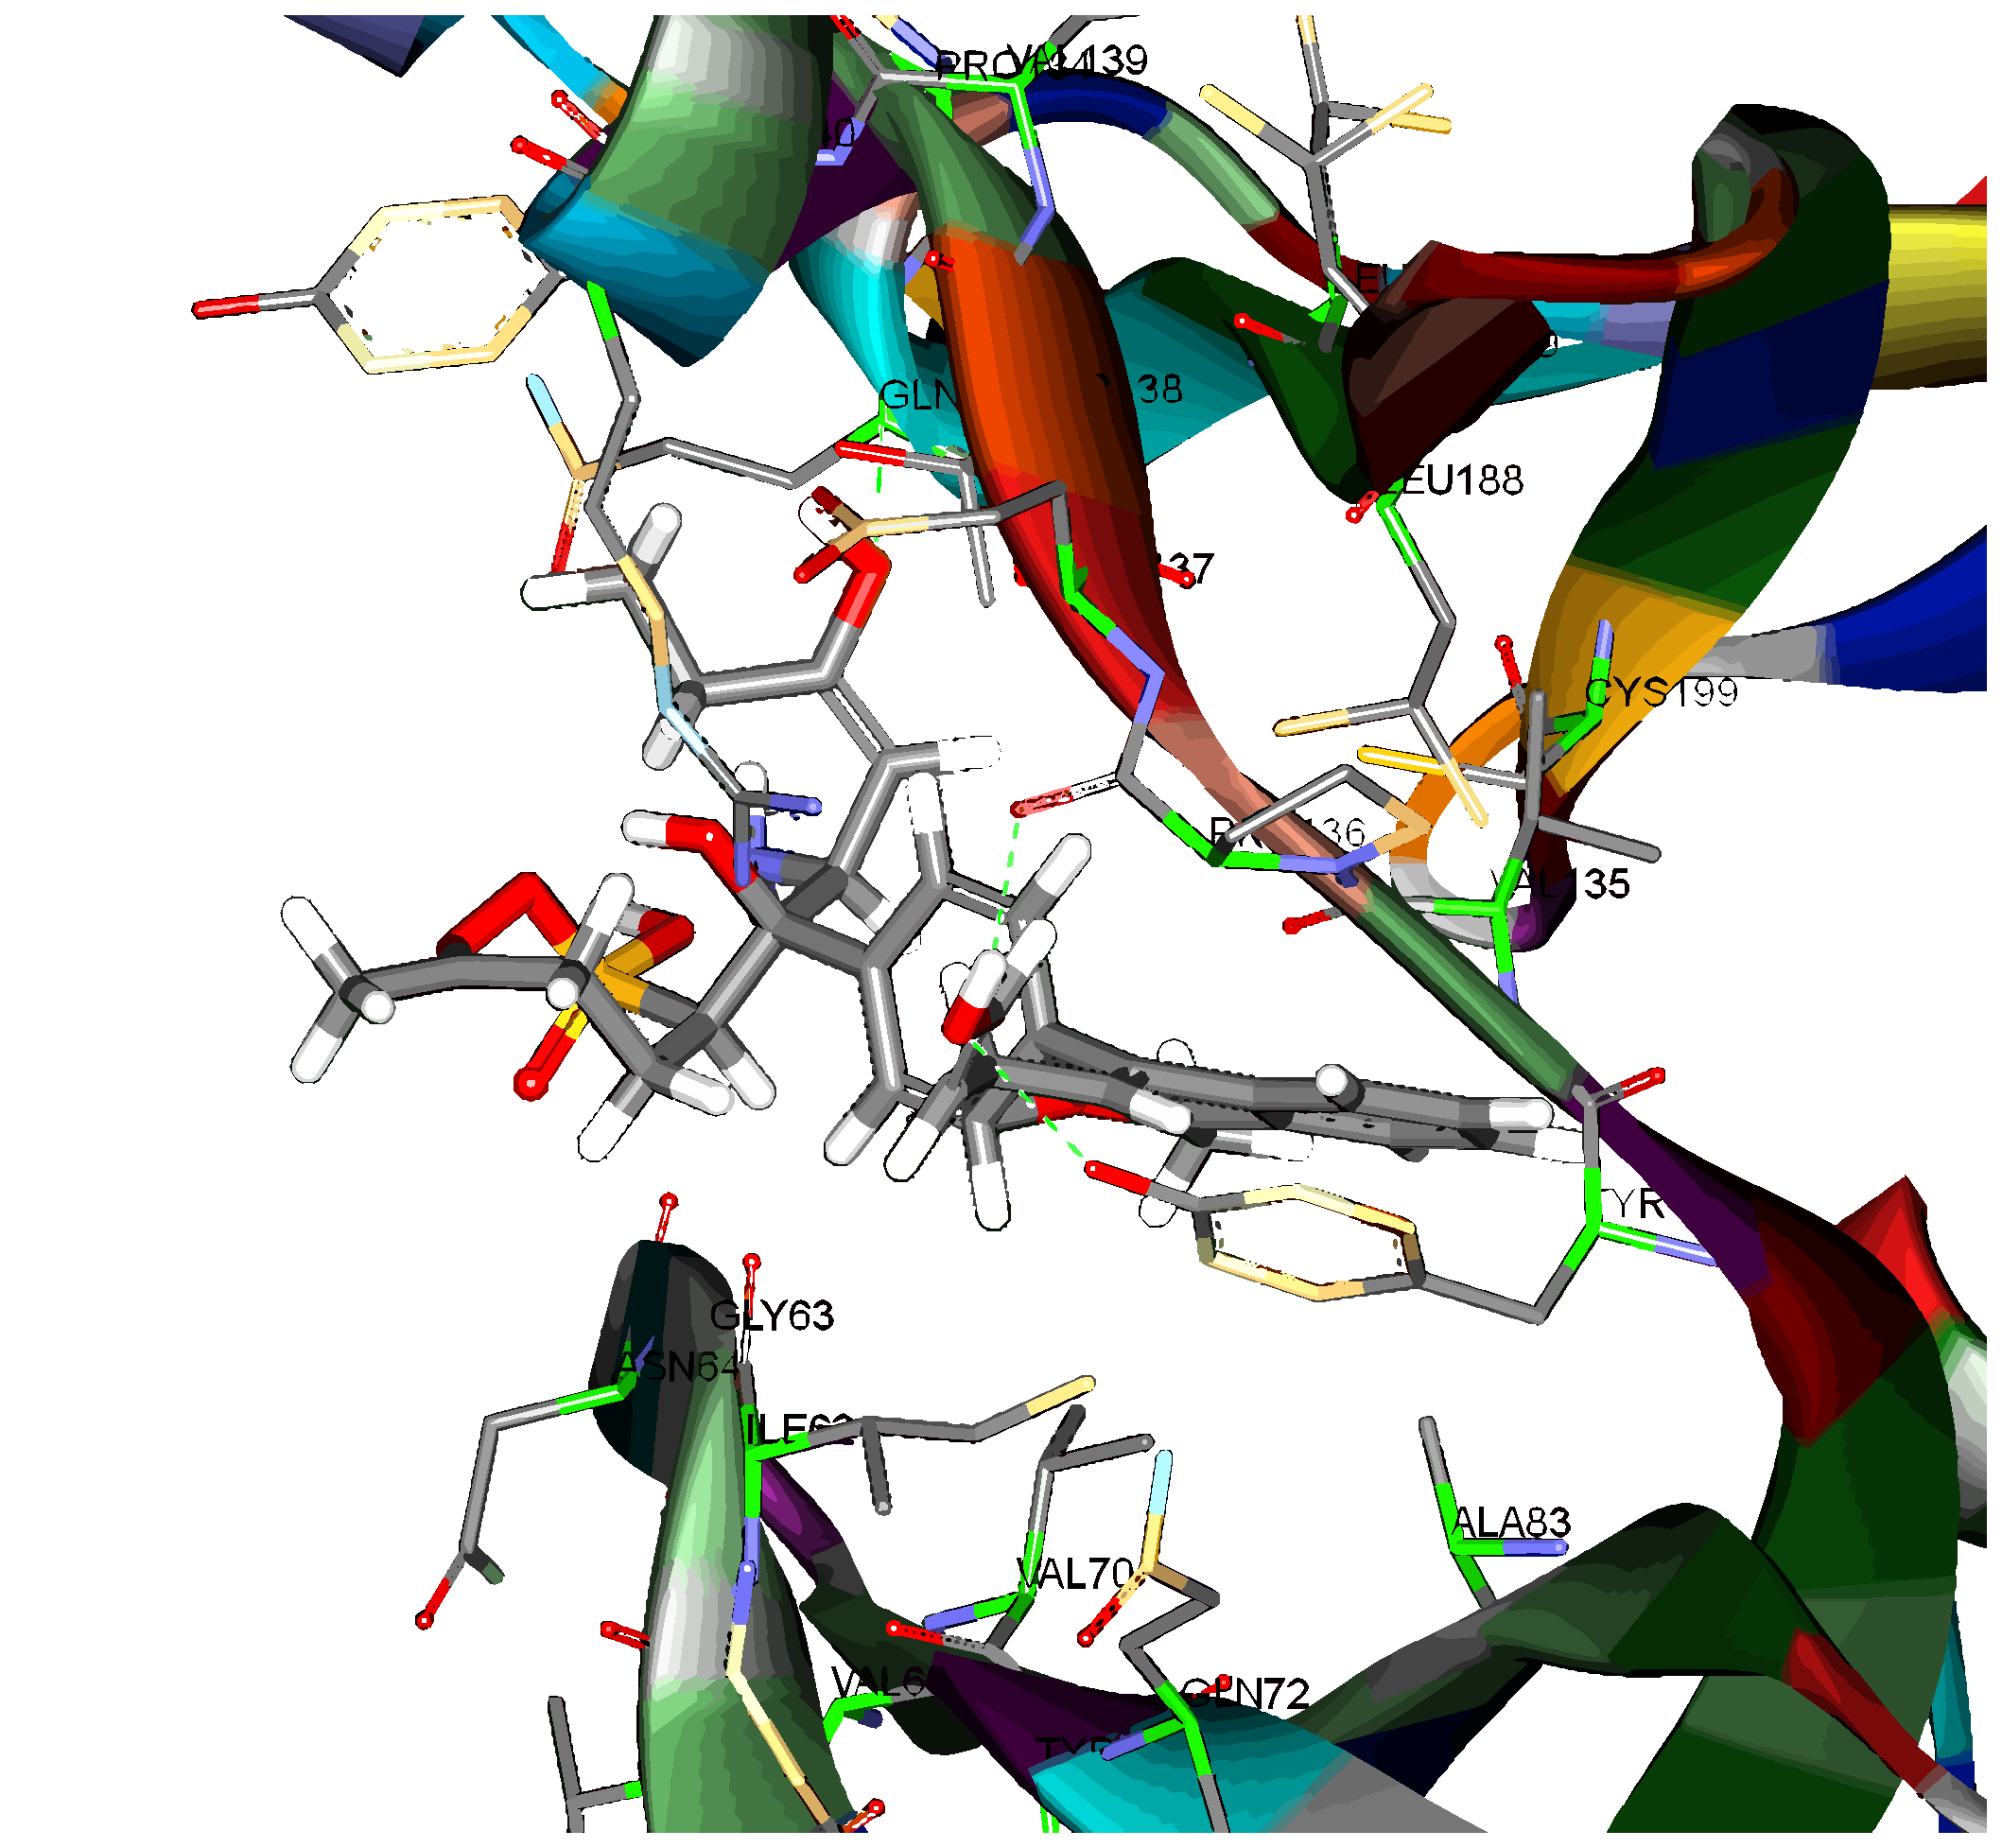
\includegraphics[width=0.31\linewidth]{Figures/Results/1J1B-ZINC01019824-AutoGrow.eps}
    \label{subfig:1J1B-ZINC01019824-AutoGrow}
  }
  \subfloat[The best ligand generated by igrow.]{
    \includegraphics[width=0.31\linewidth]{Figures/Results/1J1B-ZINC01019824-igrow.eps}
    \label{subfig:1J1B-ZINC01019824-igrow}
  }
  \caption{The initial ligand and the best ligands generated by AutoGrow and igrow, in the test case of ZINC01019824 docking to GSK3$\beta$. Hydrogen bonds are represented as dotted green lines.}
  \label{fig:BestLigands}
\end{figure*}

\begin{figure*}[t]
  \centering
  \includegraphics[width=1\linewidth]{Figures/Results/Exeution_time_with_legend.eps}
  \caption{Average execution times of AutoGrow and igrow, categorized by 3 receptors.}
  \label{fig:ExecutionTime}
\end{figure*}

%\begin{figure*}
%  \centering
%  \subfloat[GSK3$\beta$-ZINC01019824-Initial Lig.]{
%    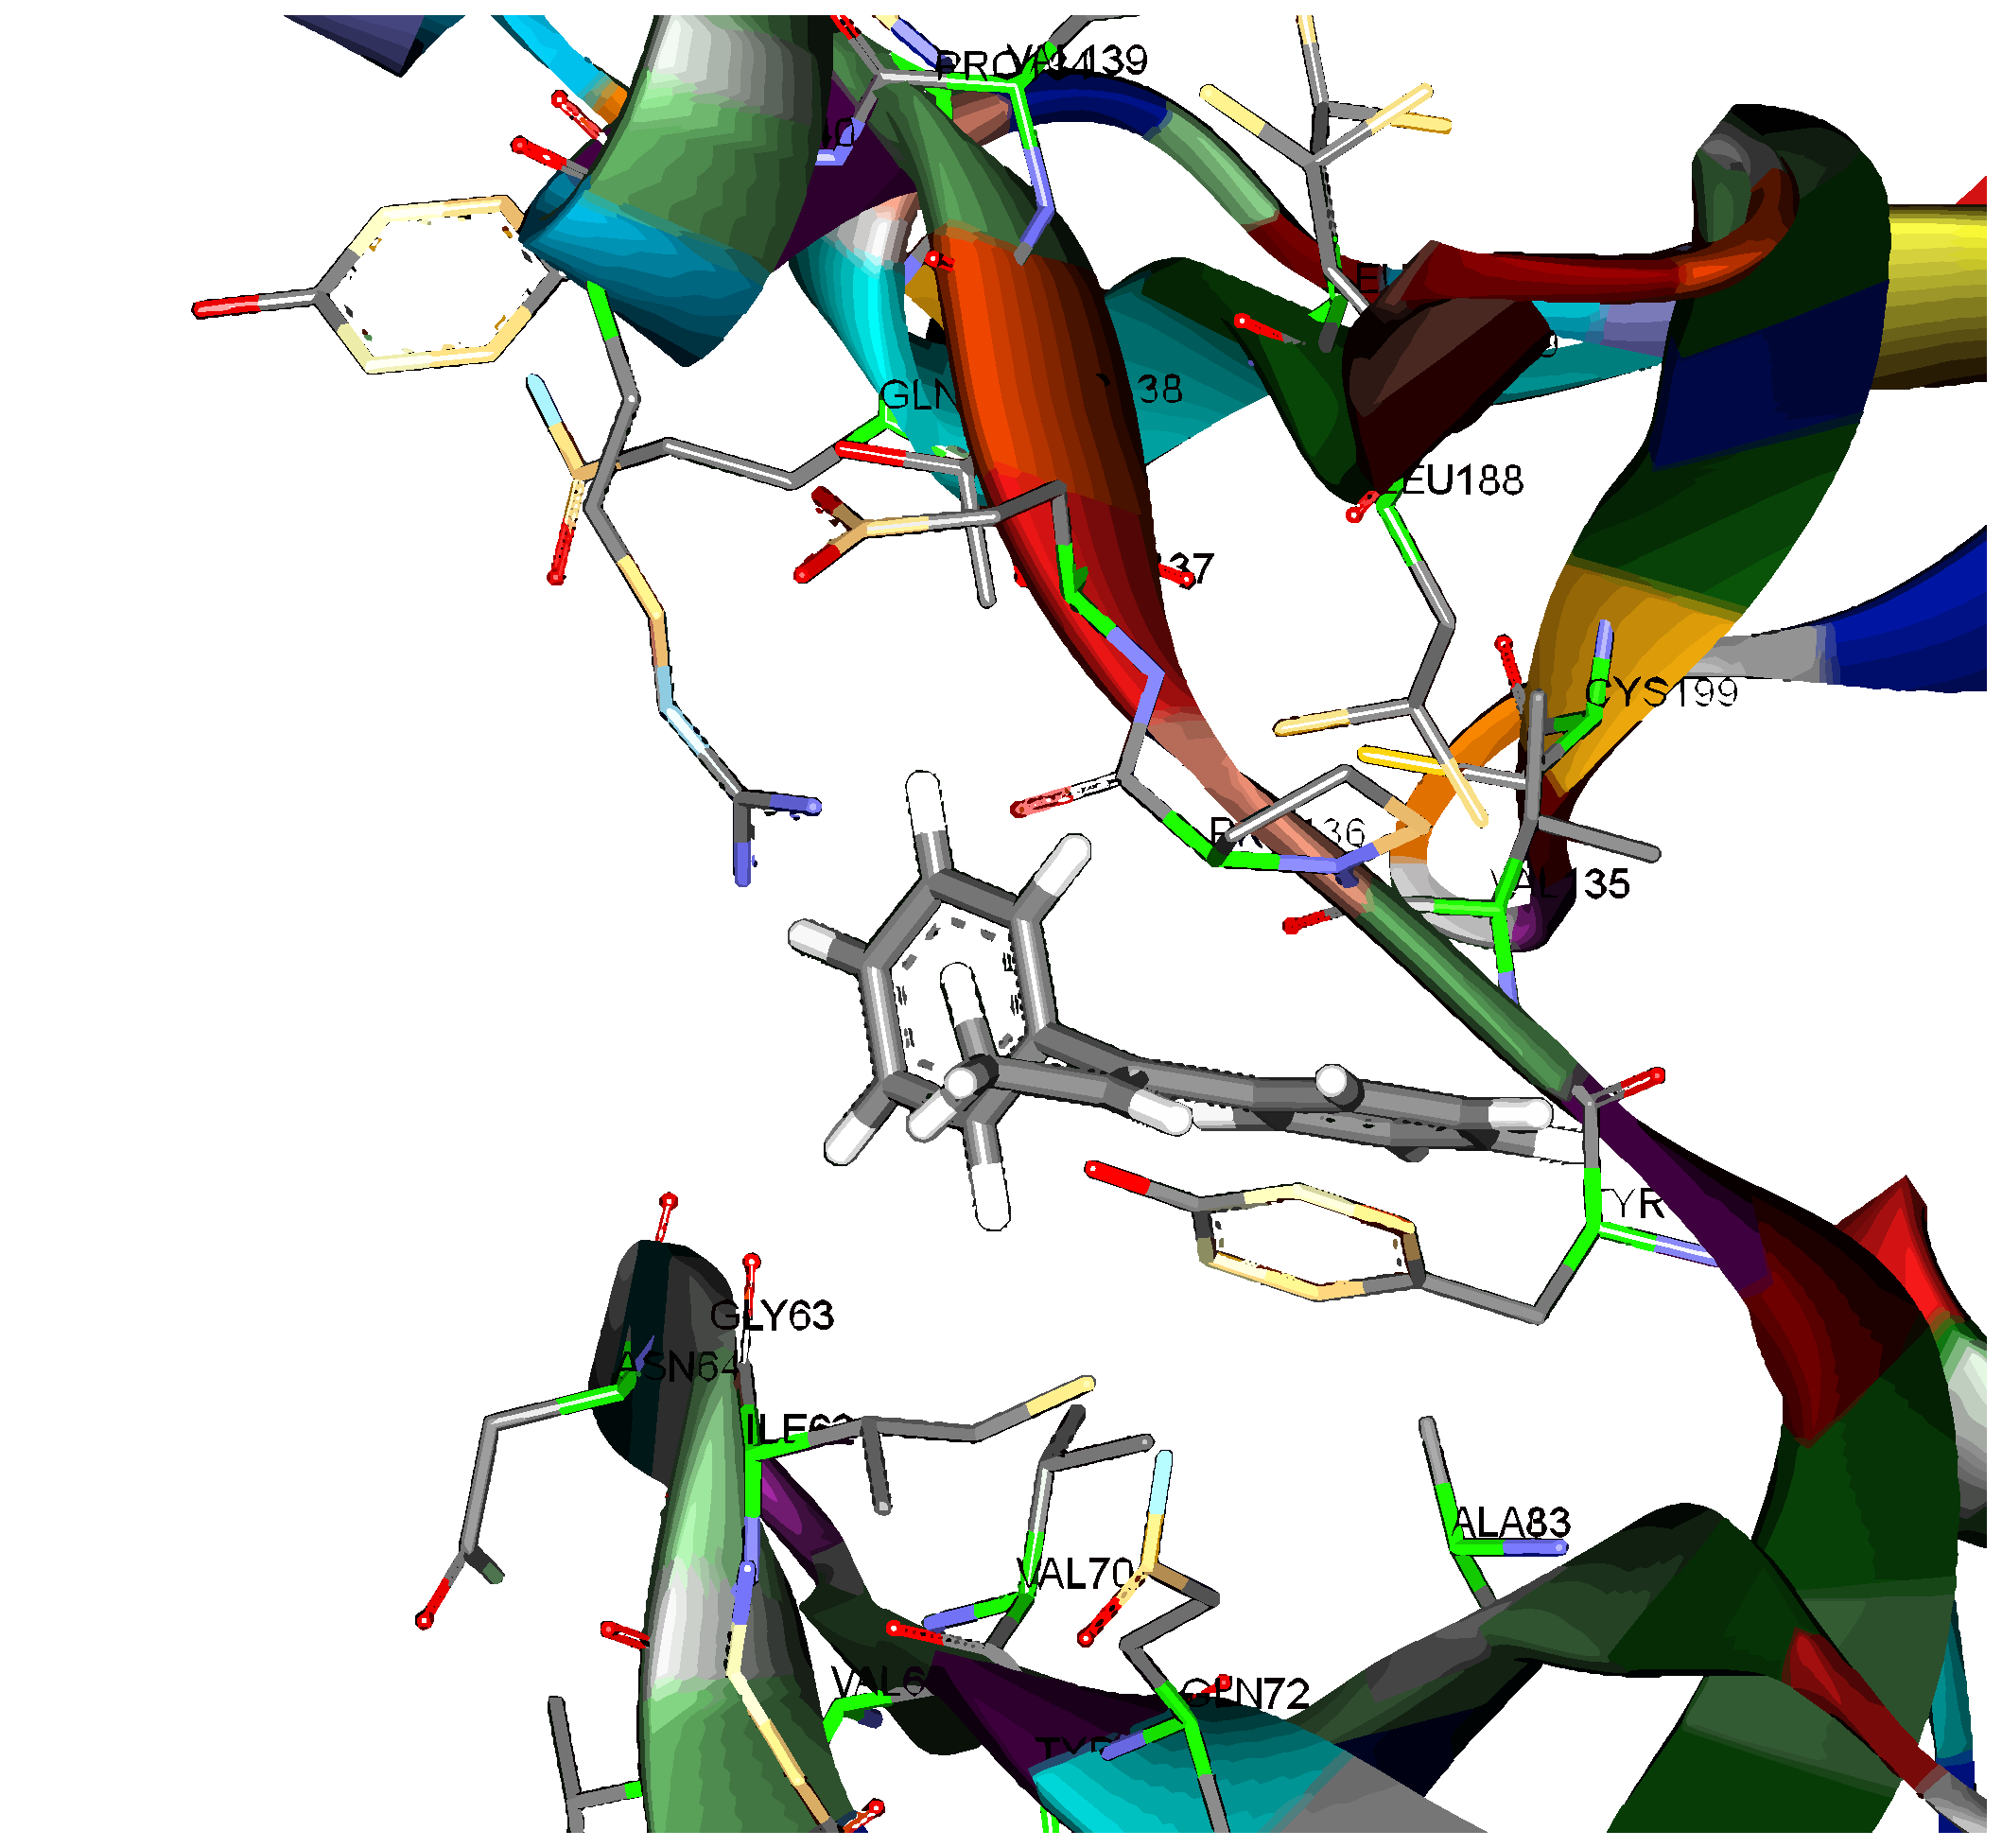
\includegraphics[width=0.31\linewidth]{Figures/Results/1J1B-ZINC01019824.eps}
%    \label{subfig:1J1B-ZINC01019824}
%  }
%  \subfloat[GSK3$\beta$-ZINC01019824-AutoGrow]{
%    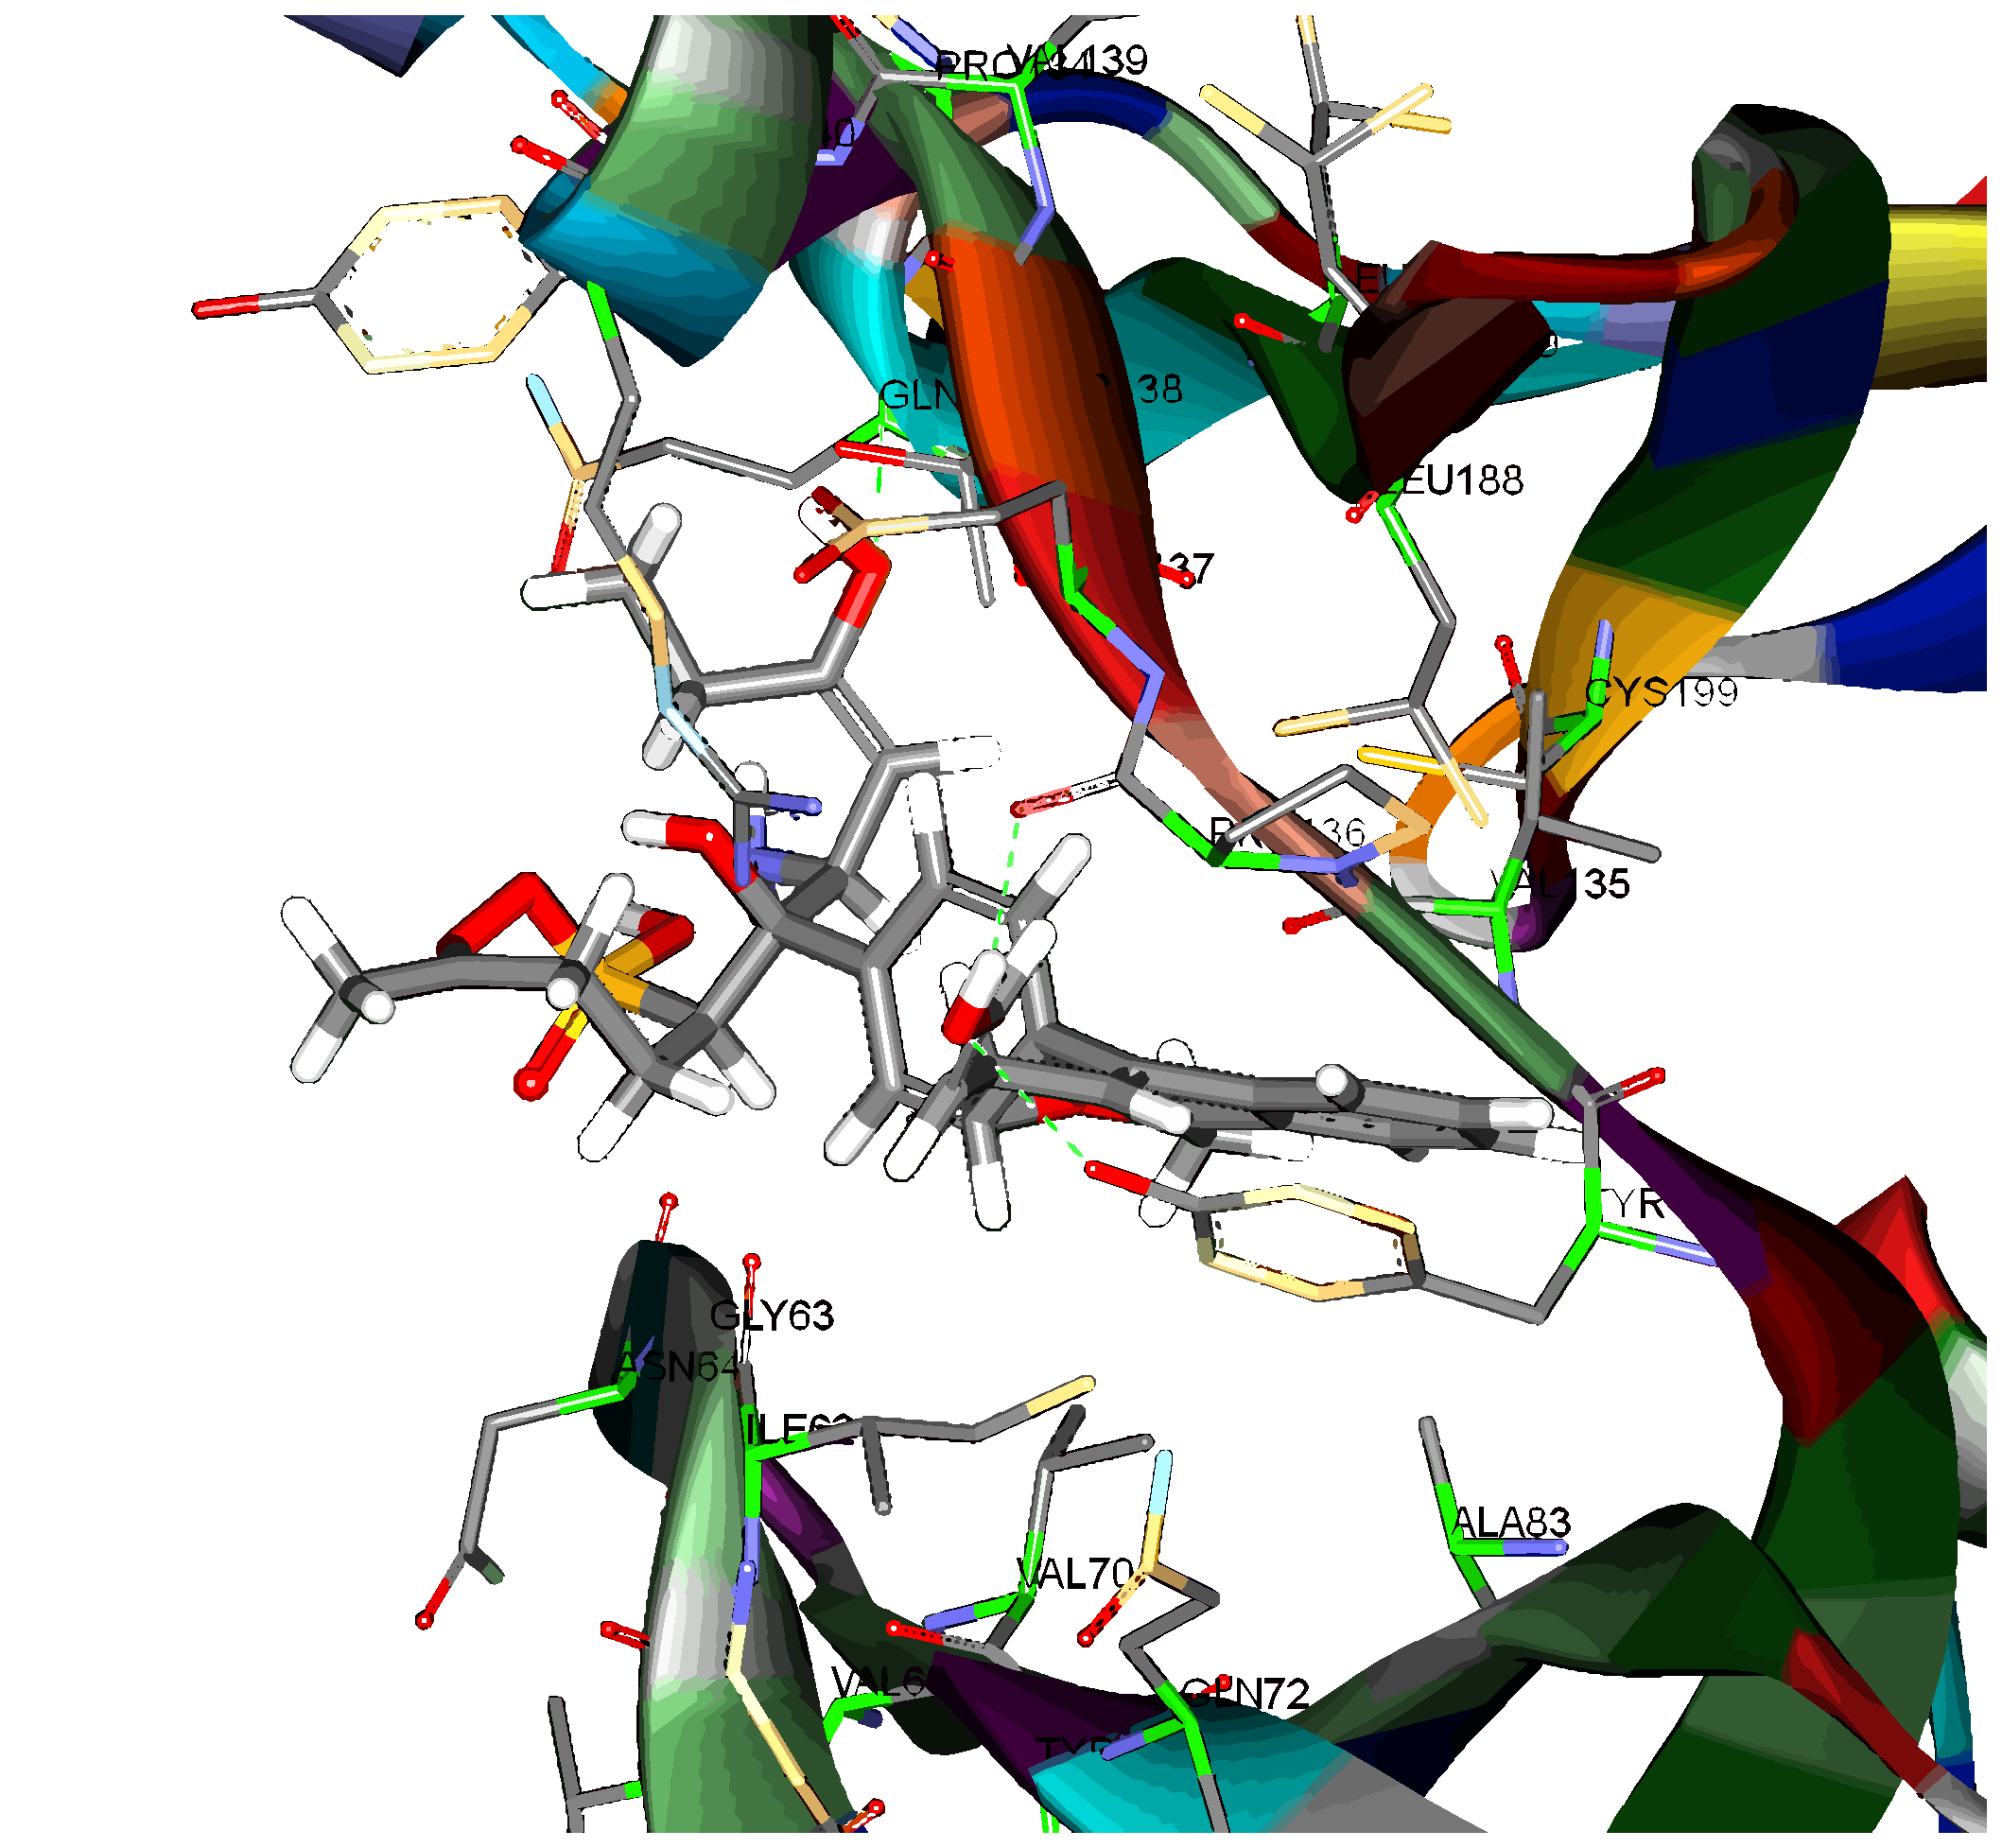
\includegraphics[width=0.31\linewidth]{Figures/Results/1J1B-ZINC01019824-AutoGrow.eps}
%    \label{subfig:1J1B-ZINC01019824-AutoGrow}
%  }
%  \subfloat[GSK3$\beta$-ZINC01019824-igrow]{
%    \includegraphics[width=0.31\linewidth]{Figures/Results/1J1B-ZINC01019824-igrow.eps}
%    \label{subfig:1J1B-ZINC01019824-igrow}
%  }
%  \subfloat[HIV RT-ZINC08442219-Initial Lig.]{
%    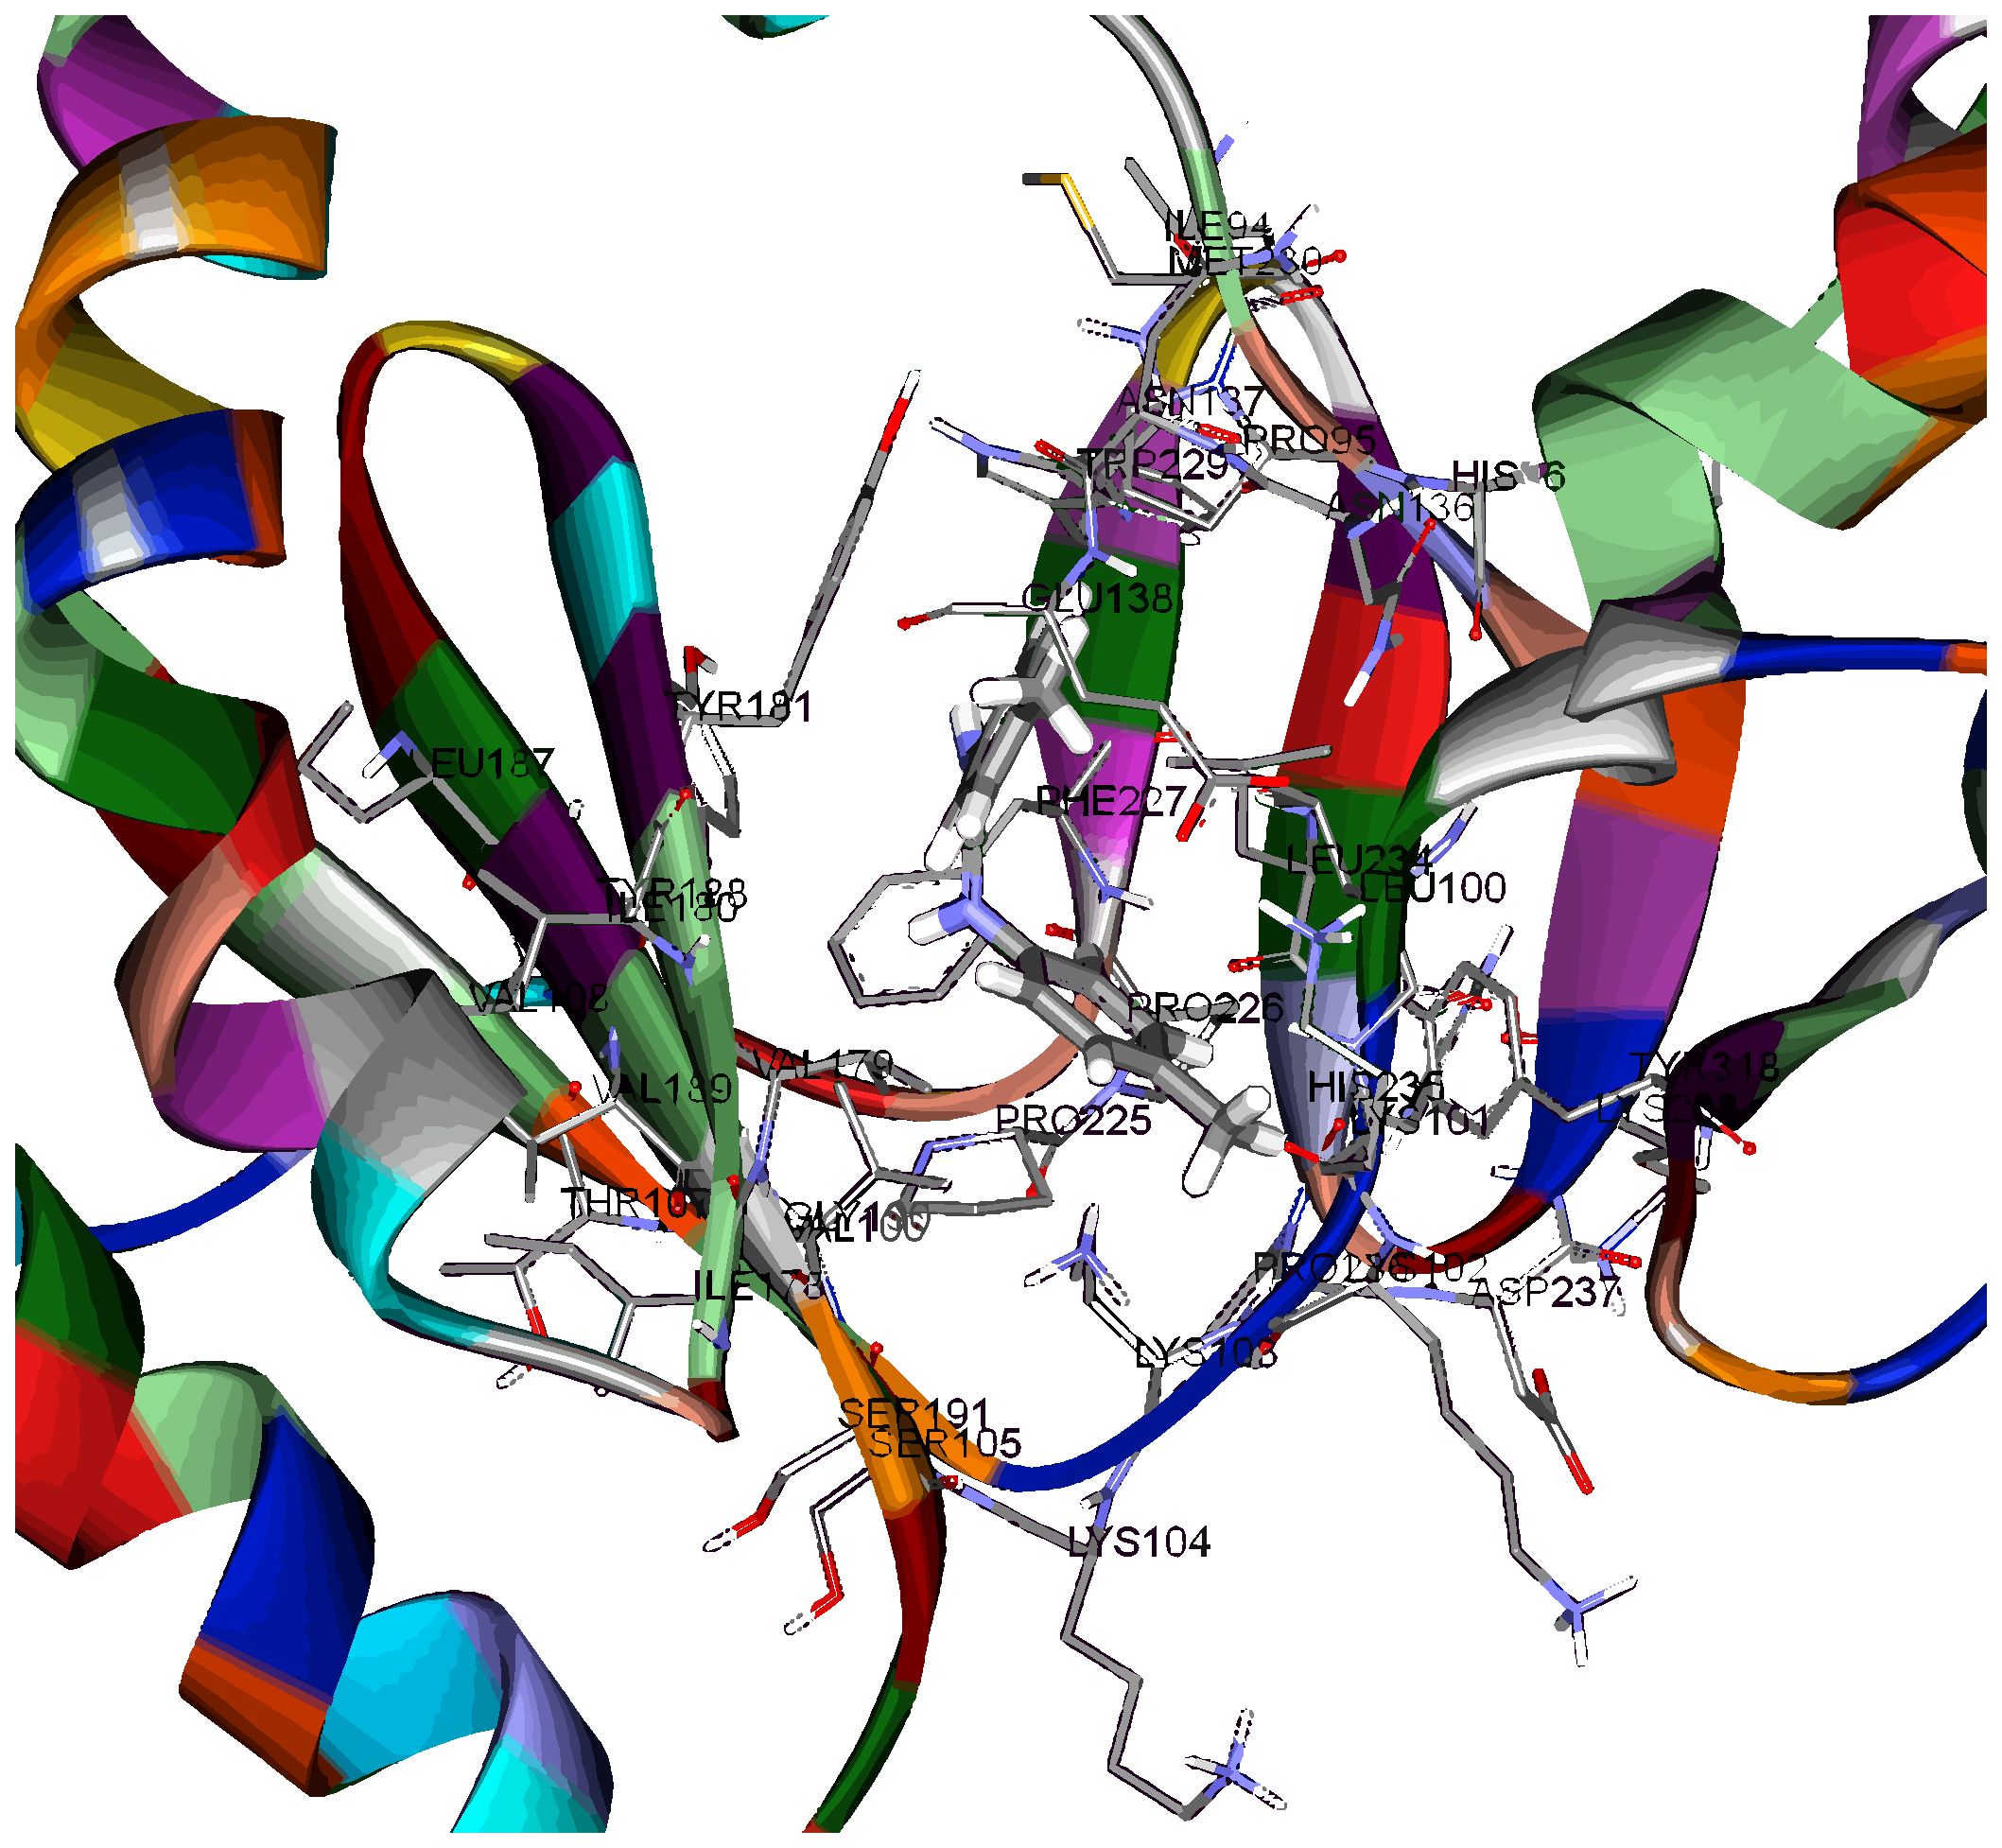
\includegraphics[width=0.31\linewidth]{Figures/Results/2ZD1-ZINC08442219.eps}
%    \label{subfig:2ZD1-ZINC08442219}
%  }
%  \subfloat[HIV RT-ZINC08442219-AutoGrow]{
%    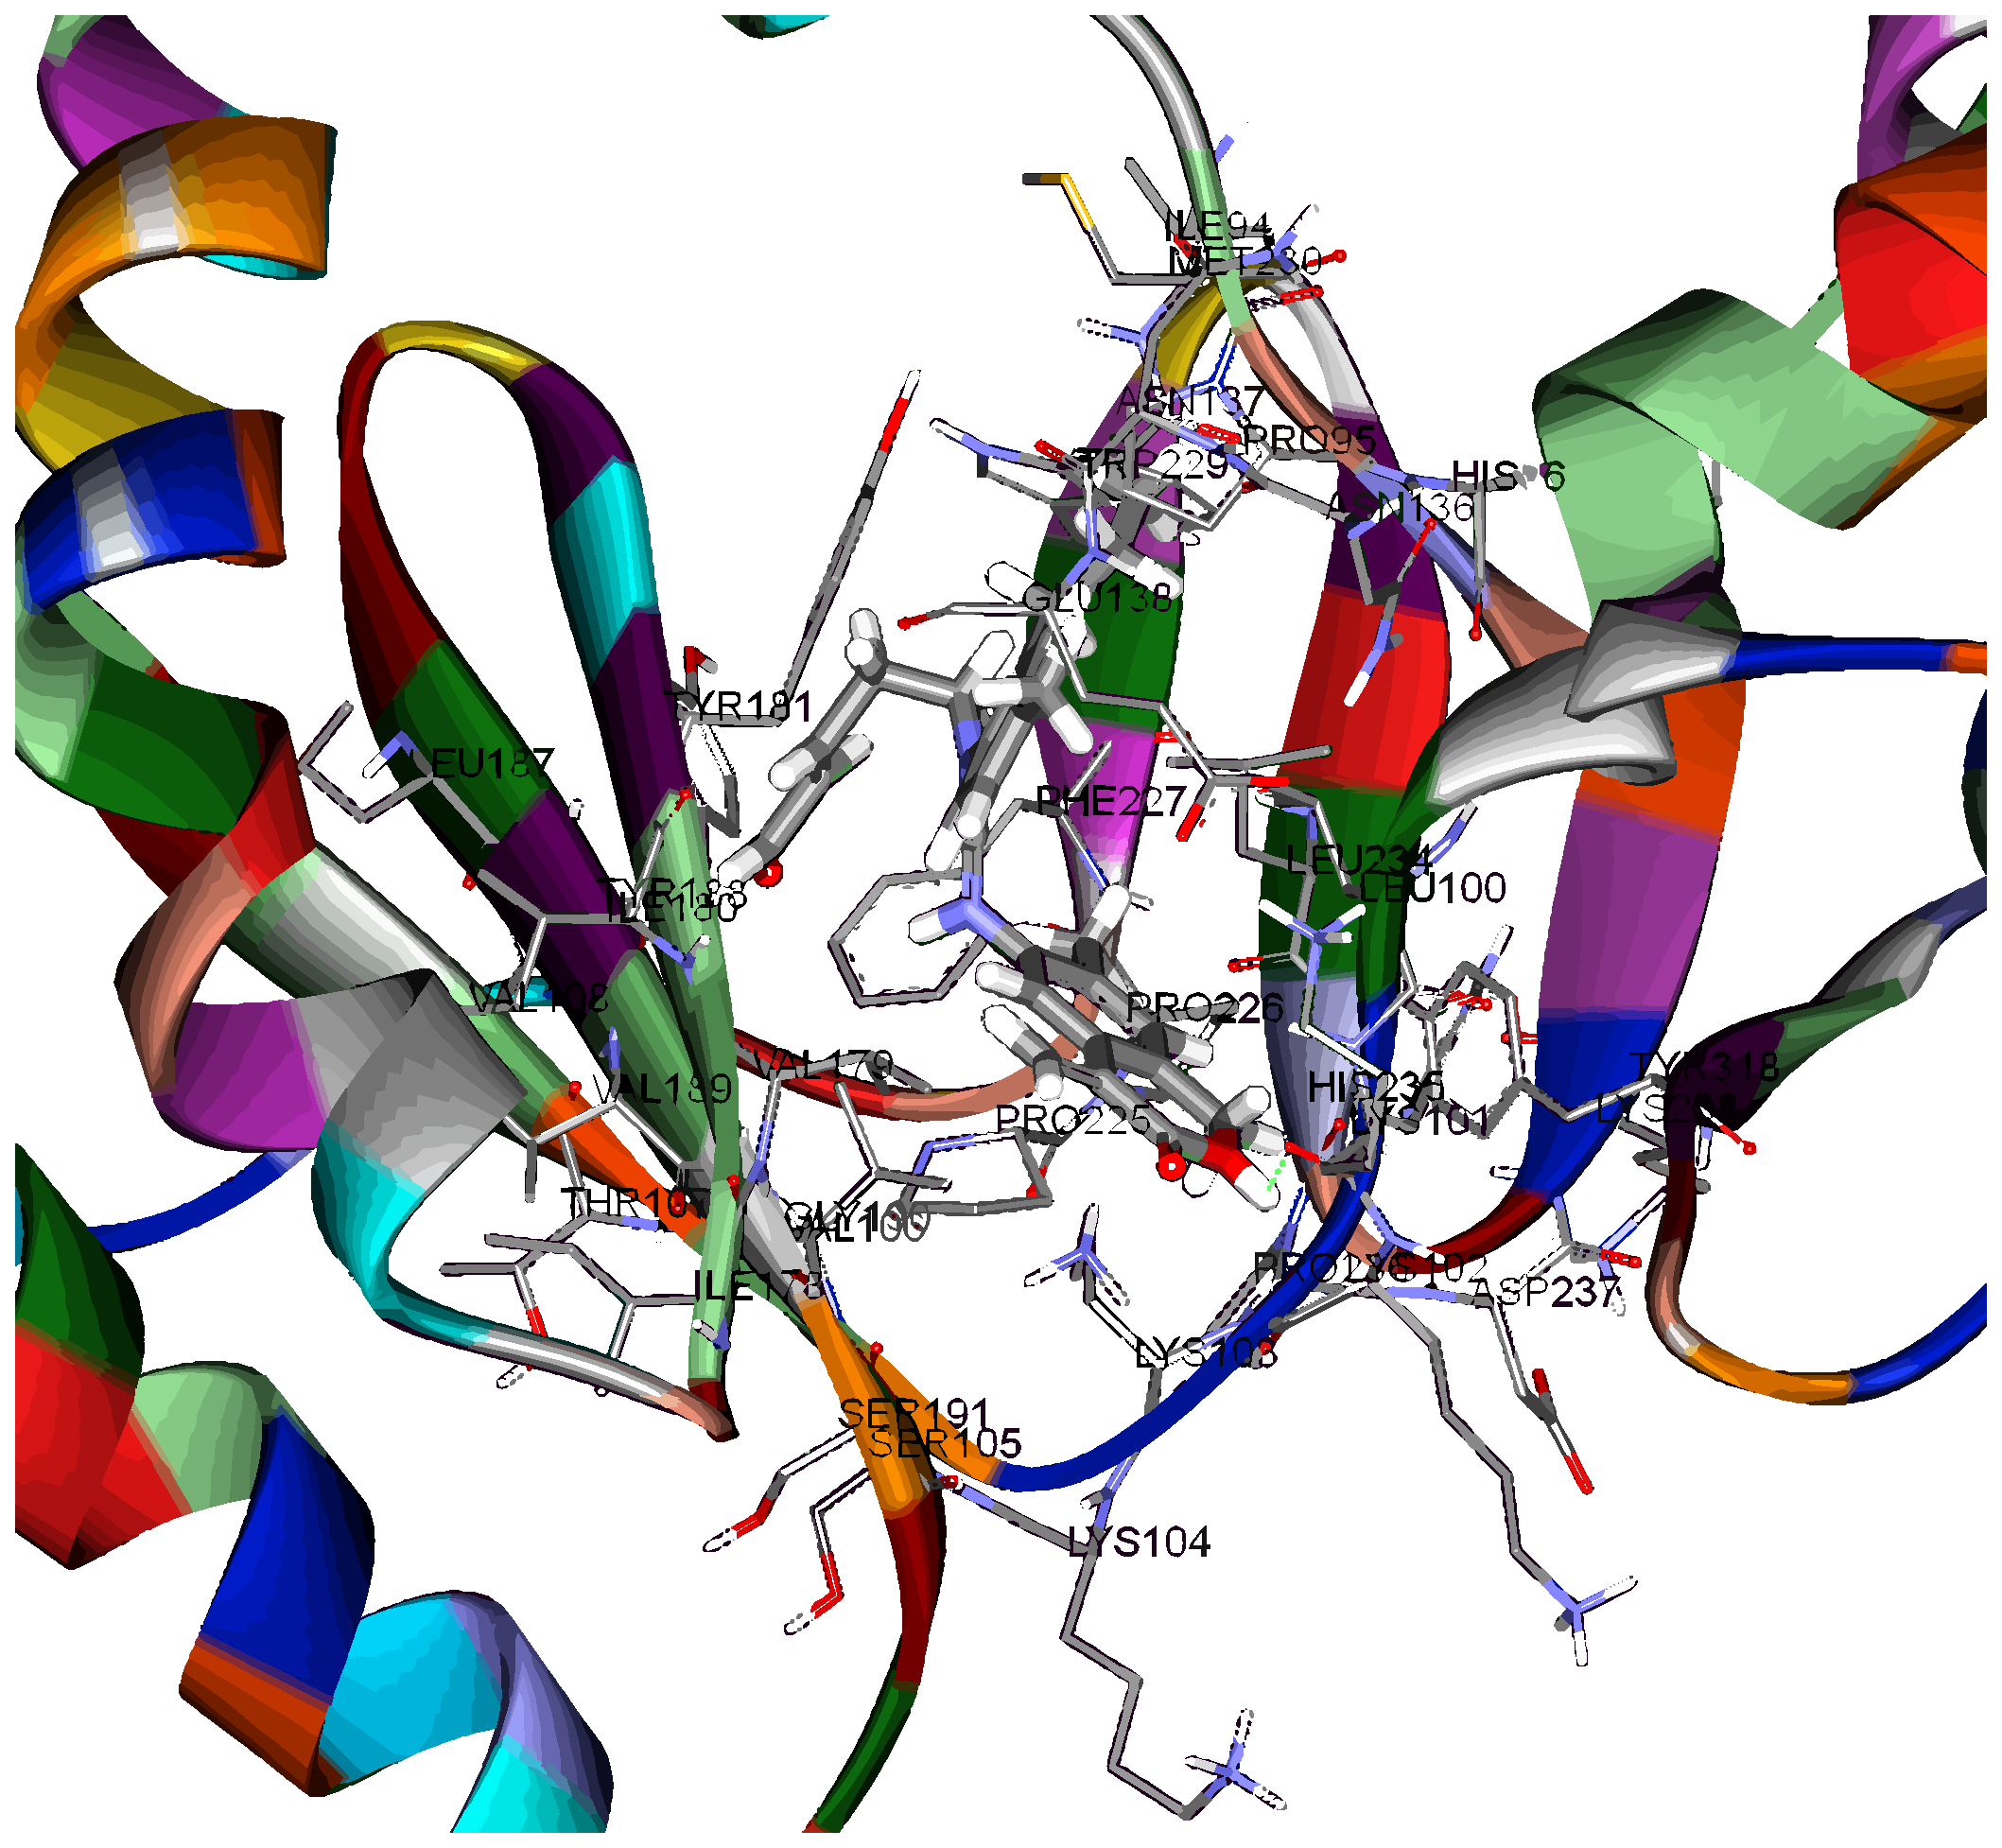
\includegraphics[width=0.31\linewidth]{Figures/Results/2ZD1-ZINC08442219-AutoGrow.eps}
%    \label{subfig:2ZD1-ZINC08442219-AutoGrow}
%  }
%  \subfloat[HIV RT-ZINC08442219-igrow]{
%    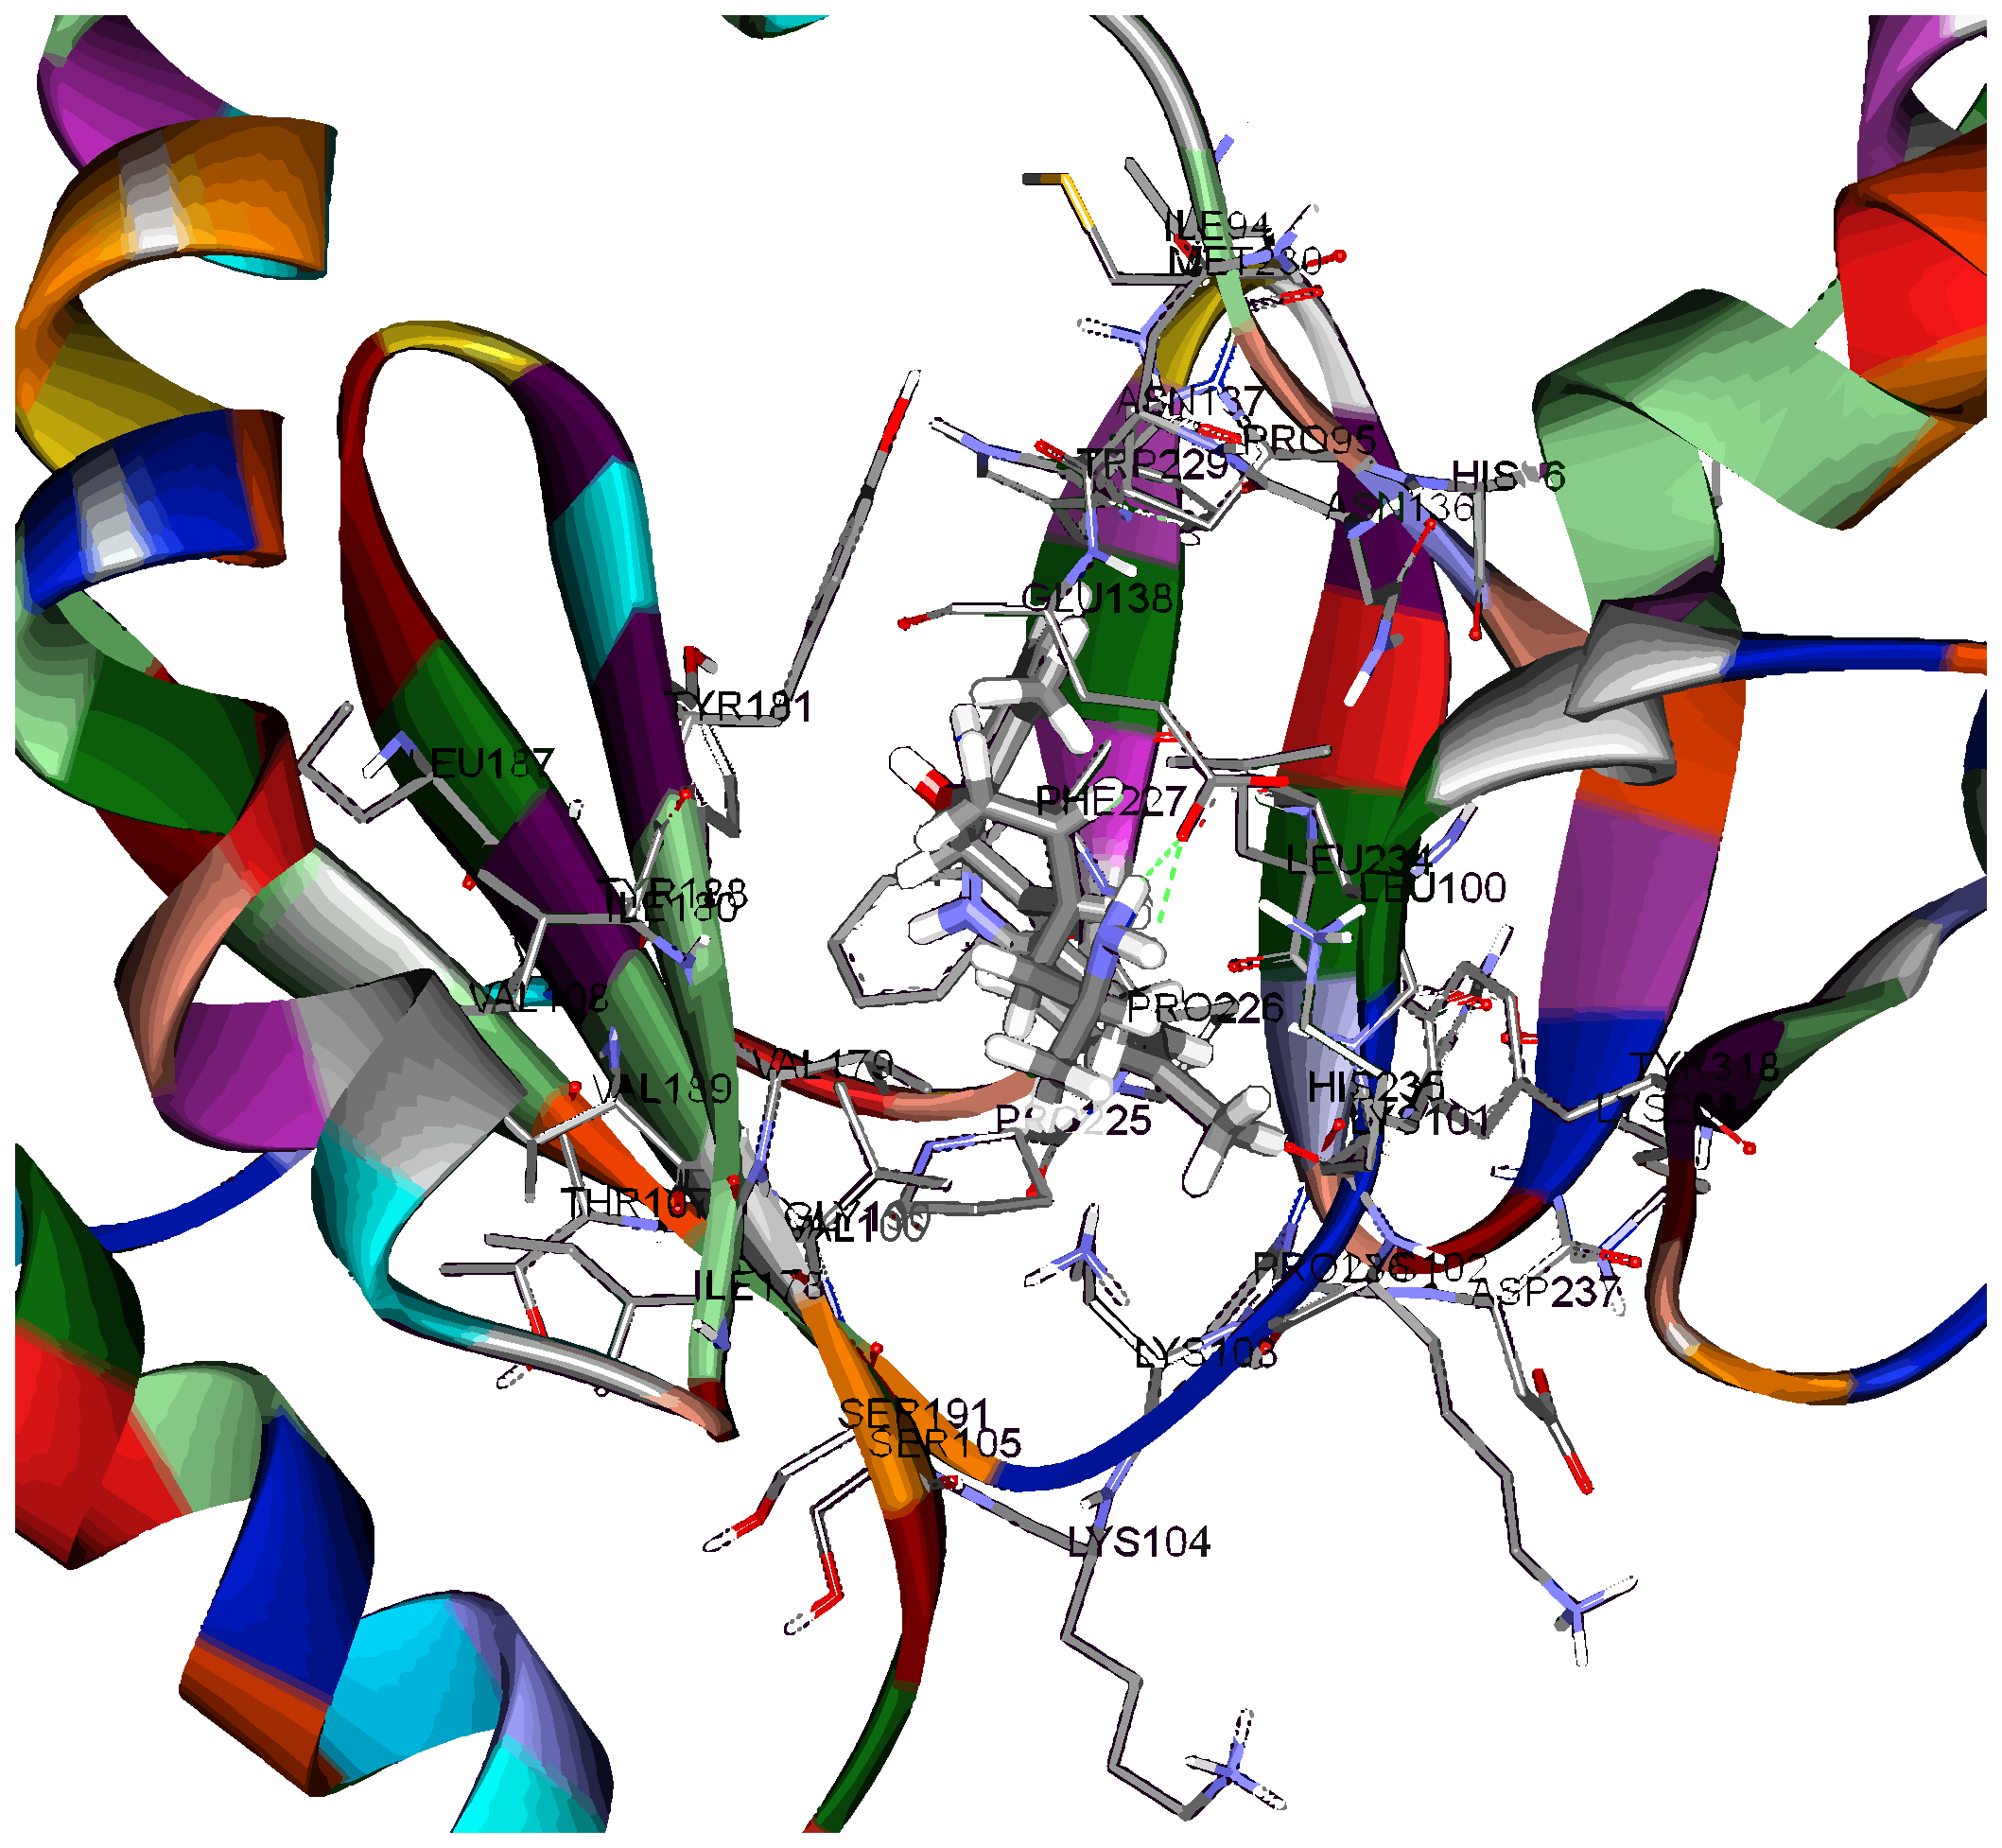
\includegraphics[width=0.31\linewidth]{Figures/Results/2ZD1-ZINC08442219-igrow.eps}
%    \label{subfig:2ZD1-ZINC08442219-igrow}
%  }
%  \subfloat[HIV PR-ZINC20030231-Initial Lig.]{
%    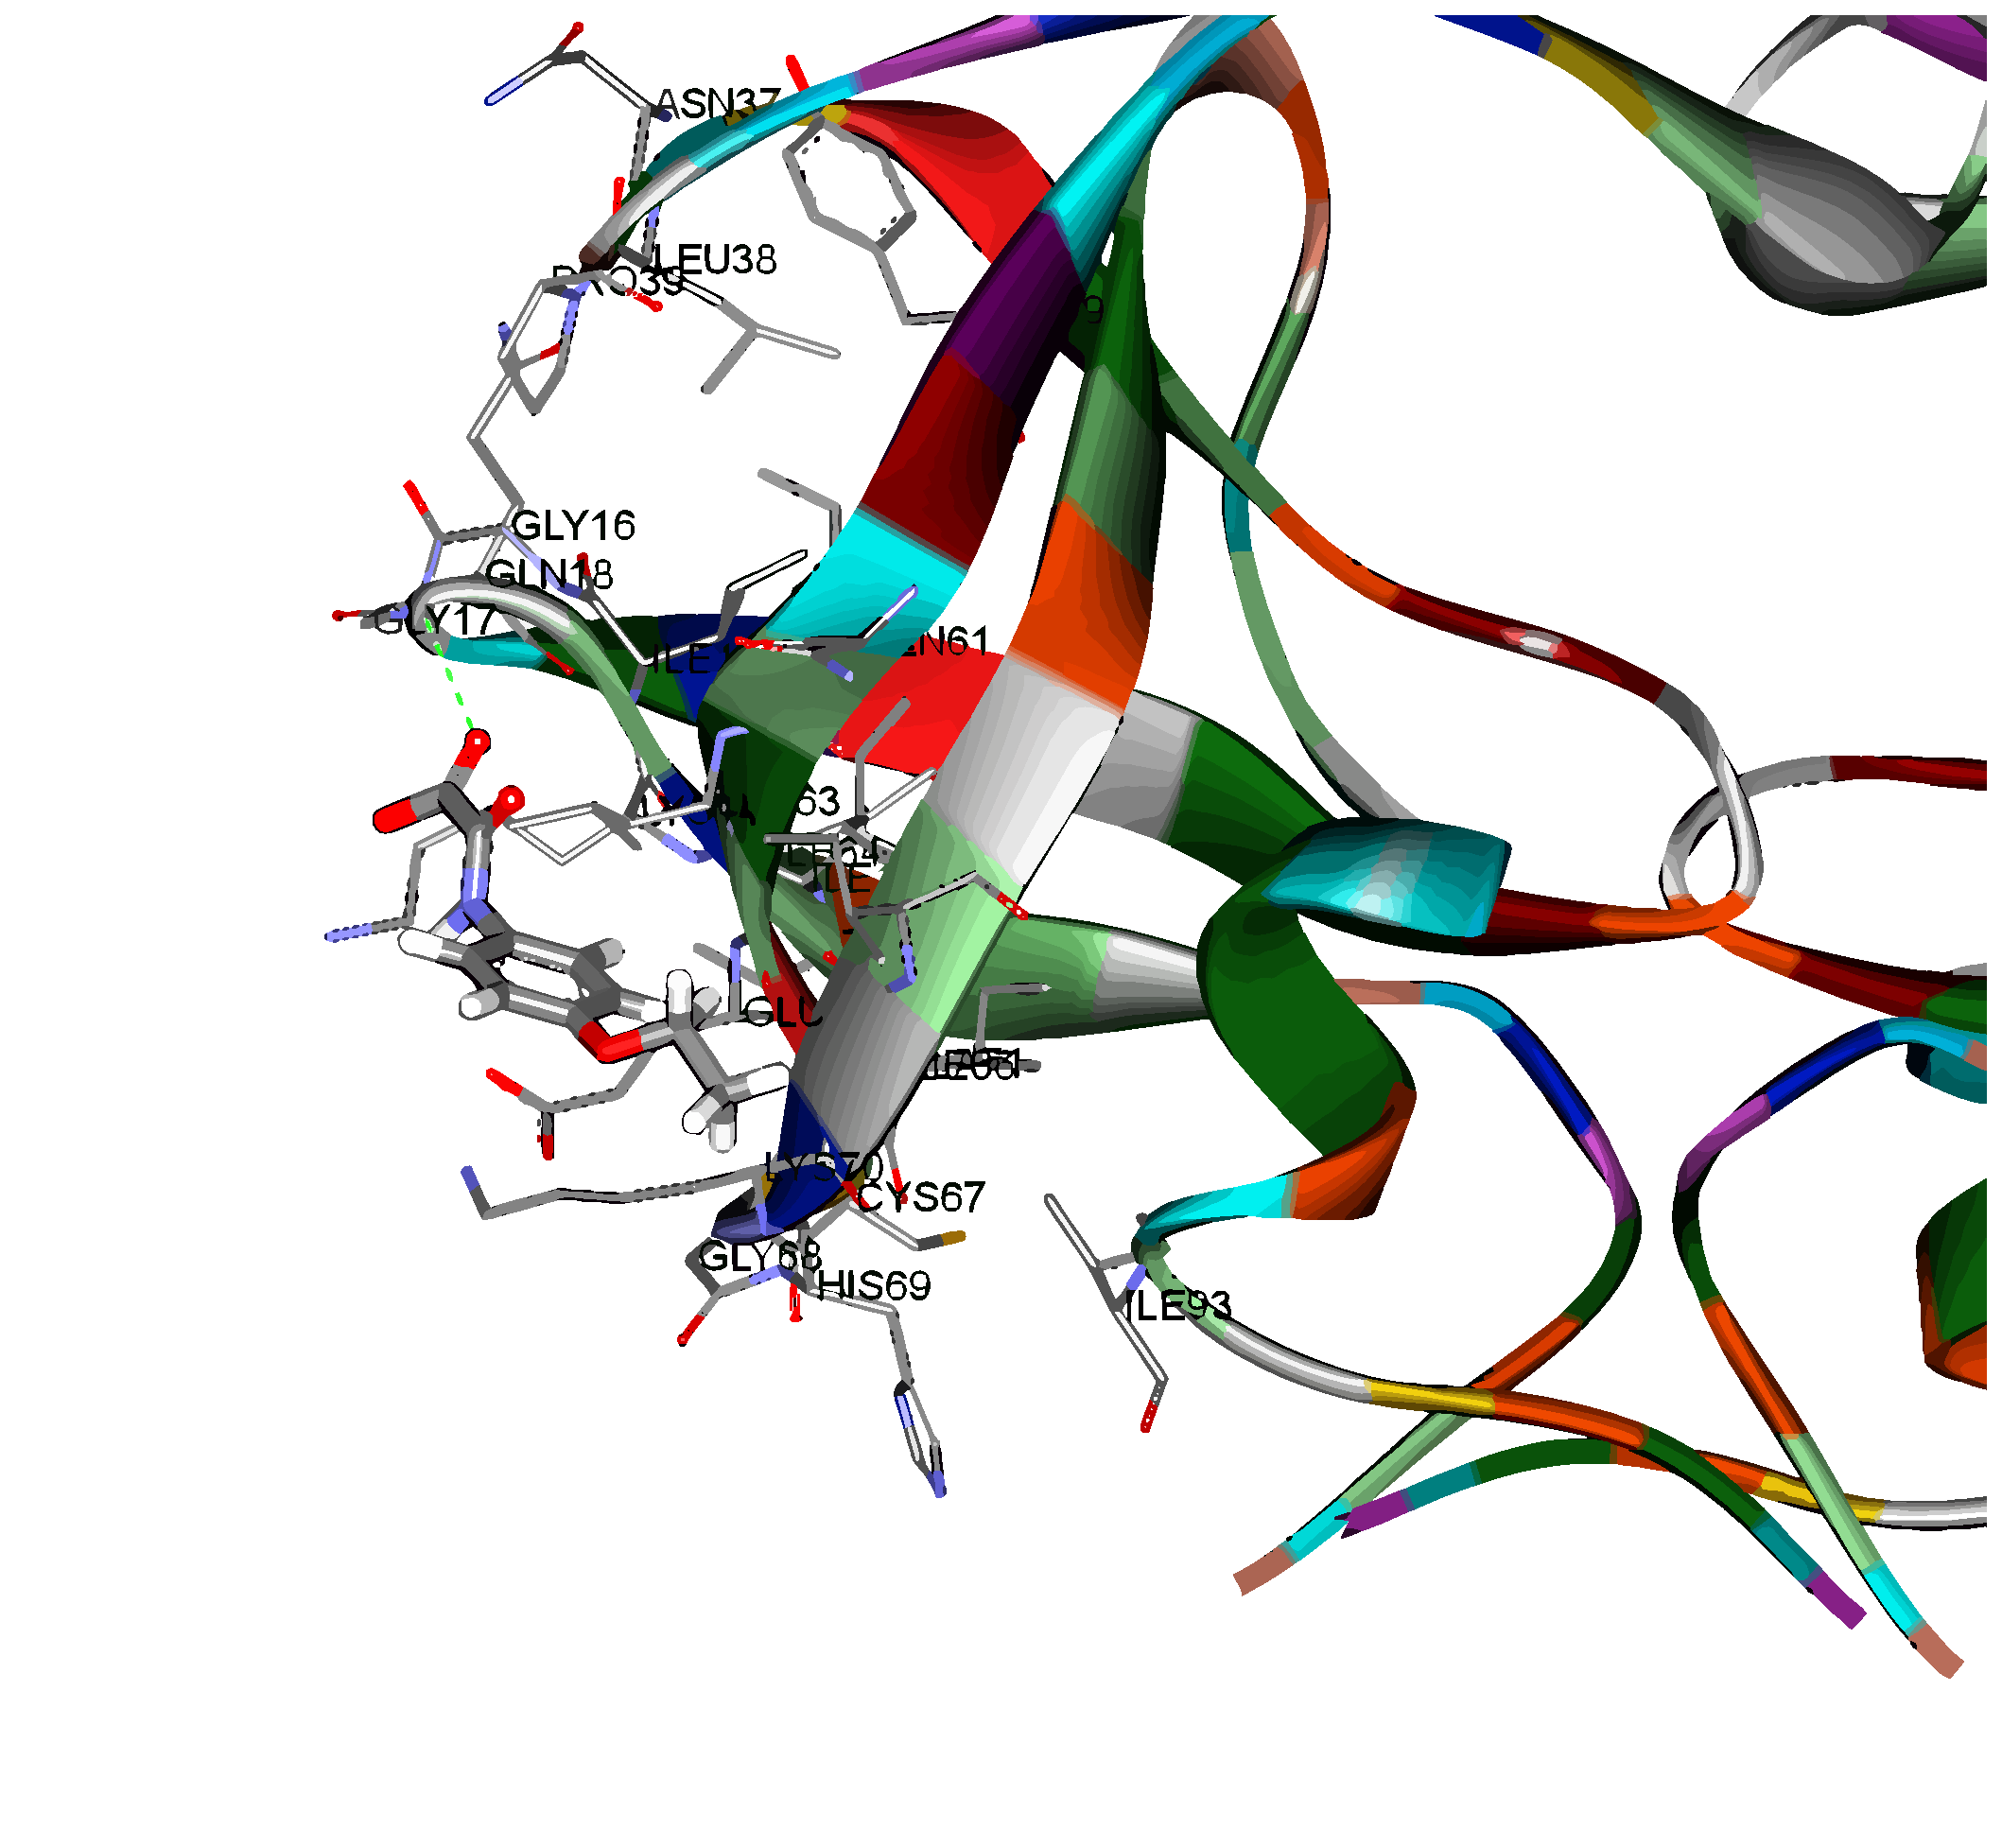
\includegraphics[width=0.31\linewidth]{Figures/Results/3KFN-ZINC20030231.eps}
%    \label{subfig:3KFN-ZINC20030231}
%  }
%  \subfloat[HIV PR-ZINC20030231-AutoGrow]{
%    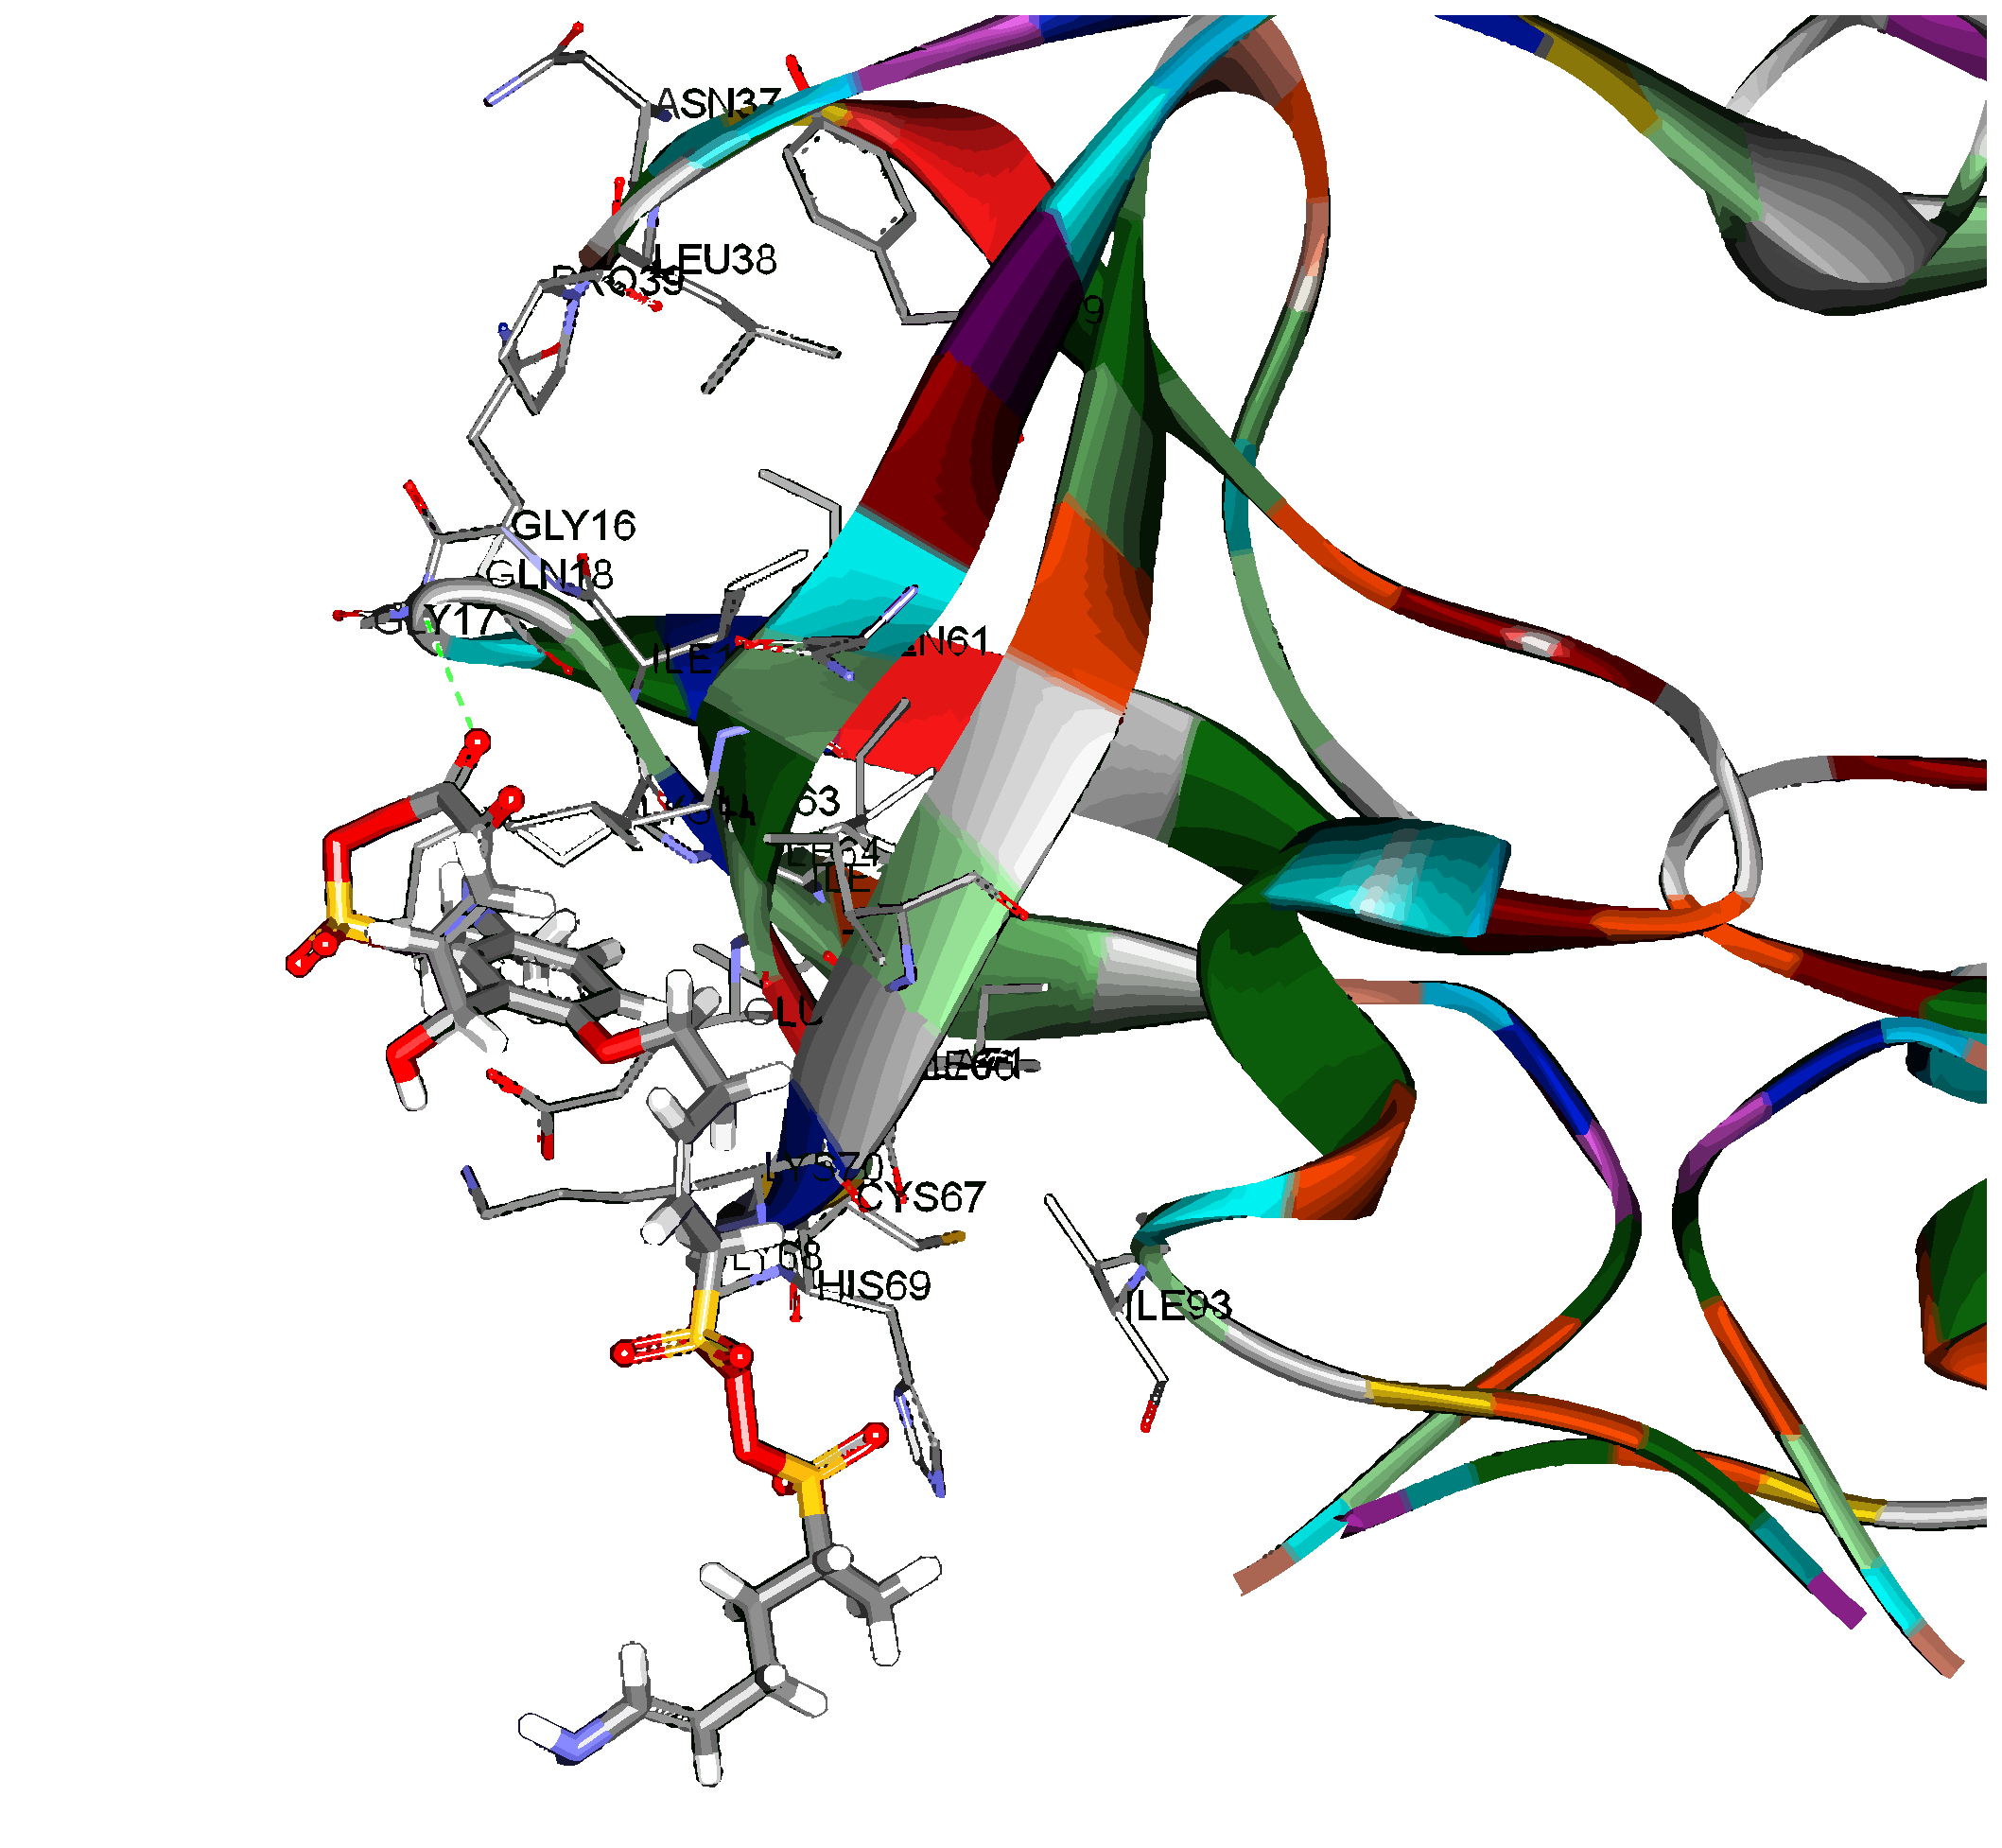
\includegraphics[width=0.31\linewidth]{Figures/Results/3KFN-ZINC20030231-AutoGrow.eps}
%    \label{subfig:3KFN-ZINC20030231-AutoGrow}
%  }
%  \subfloat[HIV PR-ZINC20030231-igrow]{
%    \includegraphics[width=0.31\linewidth]{Figures/Results/3KFN-ZINC20030231-igrow.eps}
%    \label{subfig:3KFN-ZINC20030231-igrow}
%  }
%  \caption{3 examples of the best generated ligands by AutoGrow and igrow. Hydrogen bonds are represented by dotted green lines. \subref{subfig:1J1B-ZINC01019824} -  \subref{subfig:1J1B-ZINC01019824-igrow} The best ligands generated by both programs from ZINC01019824 docking to GSK3$\beta$. \subref{subfig:2ZD1-ZINC08442219} - \subref{subfig:2ZD1-ZINC08442219-igrow} The best ligands generated by both programs from ZINC08442219 docking to HIV RT. \subref{subfig:3KFN-ZINC20030231} - \subref{subfig:3KFN-ZINC20030231-igrow} The best ligands generated by both programs from ZINC20030231 docking to HIV PR.}
%  \label{fig:BestLigands}
%\end{figure*}

%\begin{table*}
%\centering
%\begin{tabular}
%{lcccccc}
%\noalign{\smallskip}\toprule
%Receptor & \multicolumn{2}{c}{Glycogen synthase kinase 3 beta} & \multicolumn{2}{c}{HIV reverse transcriptase} & \multicolumn{2}{c}{HIV protease}\\
%Initial Ligand & \multicolumn{2}{c}{ZINC01019824} & \multicolumn{2}{c}{ZINC08442219} & \multicolumn{2}{c}{ZINC20030231}\\
%Program & AutoGrow & igrow & AutoGrow & igrow & AutoGrow & igrow\\
%\midrule
%\noalign{\smallskip}
%Free energy (kcal/mol) & -11.9 & -11.2 & -11.3 & -11.8 & -7.3 & -7.5\\
%Molecular Weight (Da) & 572 & 505 & 433 & 392 & 683 & 489\\
%\bottomrule
%\end{tabular}
%\caption{Free energies and molecular weights of the best generated ligands demonstrated in figure \ref{fig:BestLigands}.}
%\label{tab:BestLigands}
%\end{table*}

Figure \ref{subfig:1J1B-ZINC01019824} shows that the initial ligand ZINC01019824 does not form any hydrogen bond with GSK3$\beta$. It contains carbon and hydrogens atoms only, which are neither hydrogen bond donor nor acceptor. Its predicted free energy is -6.9 kcal/mol and its molecular weight is 194 Da.
Figure \ref{subfig:1J1B-ZINC01019824-AutoGrow} shows that the best ligand generated by AutoGrow is predicted to form 4 hydrogens bonds, interacting with Tyr134, Pro136, Gln185, and Asn186 of GSK3$\beta$. Its predicted free energy is -11.9 kcal/mol and its molecular weight is 572 Da, 72\% lower in free energy and 195\% larger in molecular weight than the initial ligand.
Figure \ref{subfig:1J1B-ZINC01019824-igrow} shows that the best ligand generated by igrow is predicted to form 9 hydrogens bonds, interacting with Asp133, Tyr134, Pro184, Gln185 and Asn186 of GSK3$\beta$. Its predicted free energy is -11.2 kcal/mol and its molecular weight is 505 Da, 62\% lower in free energy and 160\% larger in molecular weight than the initial ligand.

%For the second test case, the initial ligand ZINC08442219 does not form any hydrogen bond with HIV RT, as show in figure \ref{subfig:2ZD1-ZINC08442219}. The best ligand generated by AutoGrow forms 1 hydrogen bond, interacting with Lys101 of chain A of HIV RT, as show in figure \ref{subfig:2ZD1-ZINC08442219-AutoGrow}. The best ligand generated by igrow forms 2 hydrogen bonds, interacting with Glu138 of chain B of HIV RT, as show in figure \ref{subfig:2ZD1-ZINC08442219-igrow}.

%For the third test case, the initial ligand ZINC20030231 forms 1 hydrogen bond with HIV PR, interacting with Gly17 of chain A of HIV PR, as show in figure \ref{subfig:3KFN-ZINC20030231}. The best ligand generated by AutoGrow forms 2 hydrogen bonds, interacting with Lys14 and Gly17 of chain A of HIV PR, as shown in figure \ref{subfig:3KFN-ZINC20030231-AutoGrow}. The best ligand generated by igrow forms 1 hydrogen bond, interacting with Gly17 of chain A of HIV PR, as shown in figure \ref{subfig:3KFN-ZINC20030231-igrow}.

\subsection{Free Energy and Molecular Weight}
The goal of fragment-based growing strategy is not to generate one single best ligand, but a population of drug-like ligands to be shortlisted for further verifications by wet lab experiments.
Therefore it is more meaningful to dig into the average performance of the best several ligands.
Hence the predicted free energies and molecular weights of the best 5 ligands were plotted against generation number in figure \ref{fig:Best5}.

%\begin{figure*}
%  \centering
%  \subfloat[GSK3$\beta$ - TRS]{
%    \includegraphics[width=0.28\linewidth]{Figures/Results/Best5-1J1B-TRS.eps}
%    \label{subfig:Best5-1J1B-TRS}
%  }
%  \subfloat[GSK3$\beta$ - ZINC01019824]{
%    \includegraphics[width=0.28\linewidth]{Figures/Results/Best5-1J1B-ZINC01019824.eps}
%    \label{subfig:Best5-1J1B-ZINC01019824}
%  }
%  \subfloat[GSK3$\beta$ - ZINC08442219]{
%    \includegraphics[width=0.28\linewidth]{Figures/Results/Best5-1J1B-ZINC08442219.eps}
%    \label{subfig:Best5-1J1B-ZINC08442219}
%  }
%  \subfloat[GSK3$\beta$ - ZINC09365179]{
%    \includegraphics[width=0.28\linewidth]{Figures/Results/Best5-1J1B-ZINC09365179.eps}
%    \label{subfig:Best5-1J1B-ZINC09365179}
%  }
%  \subfloat[GSK3$\beta$ - ZINC18153302]{
%    \includegraphics[width=0.28\linewidth]{Figures/Results/Best5-1J1B-ZINC18153302.eps}
%    \label{subfig:Best5-1J1B-ZINC18153302}
%  }
%  \subfloat[GSK3$\beta$ - ZINC20030231]{
%    \includegraphics[width=0.28\linewidth]{Figures/Results/Best5-1J1B-ZINC20030231.eps}
%    \label{subfig:Best5-1J1B-ZINC20030231}
%  }
%  \subfloat[HIV RT - T27]{
%    \includegraphics[width=0.28\linewidth]{Figures/Results/Best5-2ZD1-T27.eps}
%    \label{subfig:Best5-2ZD1-T27}
%  }
%  \subfloat[HIV RT - ZINC01019824]{
%    \includegraphics[width=0.28\linewidth]{Figures/Results/Best5-2ZD1-ZINC01019824.eps}
%    \label{subfig:Best5-2ZD1-ZINC01019824}
%  }
%  \subfloat[HIV RT - ZINC08442219]{
%    \includegraphics[width=0.28\linewidth]{Figures/Results/Best5-2ZD1-ZINC08442219.eps}
%    \label{subfig:Best5-2ZD1-ZINC08442219}
%  }
%  \subfloat[HIV RT - ZINC09365179]{
%    \includegraphics[width=0.28\linewidth]{Figures/Results/Best5-2ZD1-ZINC09365179.eps}
%    \label{subfig:Best5-2ZD1-ZINC09365179}
%  }
%  \subfloat[HIV RT - ZINC18153302]{
%    \includegraphics[width=0.28\linewidth]{Figures/Results/Best5-2ZD1-ZINC18153302.eps}
%    \label{subfig:Best5-2ZD1-ZINC18153302}
%  }
%  \subfloat[HIV RT - ZINC20030231]{
%    \includegraphics[width=0.28\linewidth]{Figures/Results/Best5-2ZD1-ZINC20030231.eps}
%    \label{subfig:Best5-2ZD1-ZINC20030231}
%  }
%  \caption{Average free energies and molecular weights of the best 5 ligands generated by AutoGrow and igrow of each generation. Generation 0 refers to the initial ligand. Blue curve: average free energies of the best 5 ligands generated by AutoGrow. Green curve: average free energies of the best 5 ligands generated by igrow. Red curve: average molecular weights of the best 5 ligands generated by AutoGrow. Purple curve: average molecular weights of the best 5 ligands generated by igrow. \subref{subfig:Best5-1J1B-TRS} - \subref{subfig:Best5-1J1B-ZINC20030231} 6 initial ligands docking to glycogen synthase kinase 3 beta. \subref{subfig:Best5-2ZD1-T27} - \subref{subfig:Best5-2ZD1-ZINC20030231} 6 initial ligands docking to HIV reverse transcriptase.}
%  \label{fig:Best5-1J1B-2ZD1}
%\end{figure*}

%\begin{figure*}[ht!]
%  \centering
%  \subfloat[HIV PR - 4DX]{
%    \includegraphics[width=0.28\linewidth]{Figures/Results/Best5-3KFN-4DX.eps}
%    \label{subfig:Best5-3KFN-4DX}
%  }
%  \subfloat[HIV PR - ZINC01019824]{
%    \includegraphics[width=0.28\linewidth]{Figures/Results/Best5-3KFN-ZINC01019824.eps}
%    \label{subfig:Best5-3KFN-ZINC01019824}
%  }
%  \subfloat[HIV PR - ZINC08442219]{
%    \includegraphics[width=0.28\linewidth]{Figures/Results/Best5-3KFN-ZINC08442219.eps}
%    \label{subfig:Best5-3KFN-ZINC08442219}
%  }
%  \subfloat[HIV PR - ZINC09365179]{
%    \includegraphics[width=0.28\linewidth]{Figures/Results/Best5-3KFN-ZINC09365179.eps}
%    \label{subfig:Best5-3KFN-ZINC09365179}
%  }
%  \subfloat[HIV PR - ZINC18153302]{
%    \includegraphics[width=0.28\linewidth]{Figures/Results/Best5-3KFN-ZINC18153302.eps}
%    \label{subfig:Best5-3KFN-ZINC18153302}
%  }
%  \subfloat[HIV RT - ZINC20030231]{
%    \includegraphics[width=0.28\linewidth]{Figures/Results/Best5-3KFN-ZINC20030231.eps}
%    \label{subfig:Best5-3KFN-ZINC20030231}
%  }
%  \caption{\subref{subfig:Best5-3KFN-4DX} - \subref{subfig:Best5-3KFN-ZINC20030231} 6 initial ligands docking to HIV protease. The legends are the same as figure \ref{fig:Best5-1J1B-2ZD1}.}
%  \label{fig:Best5-3KFN}
%\end{figure*}

\subsection{Execution Time}
We also measured the execution times of AutoGrow and igrow.
Since all the test cases were run for 9 times, their average execution times are shown in figure \ref{fig:ExecutionTime}.

%\begin{figure*}[ht!]
%  \centering
%  \subfloat[GSK3$\beta$]{
%    \includegraphics[width=0.31\linewidth]{Figures/Results/ExecutionTime-1J1B.eps}
%    \label{subfig:ExecutionTime-1J1B}
%  }
%  \subfloat[HIV RT]{
%    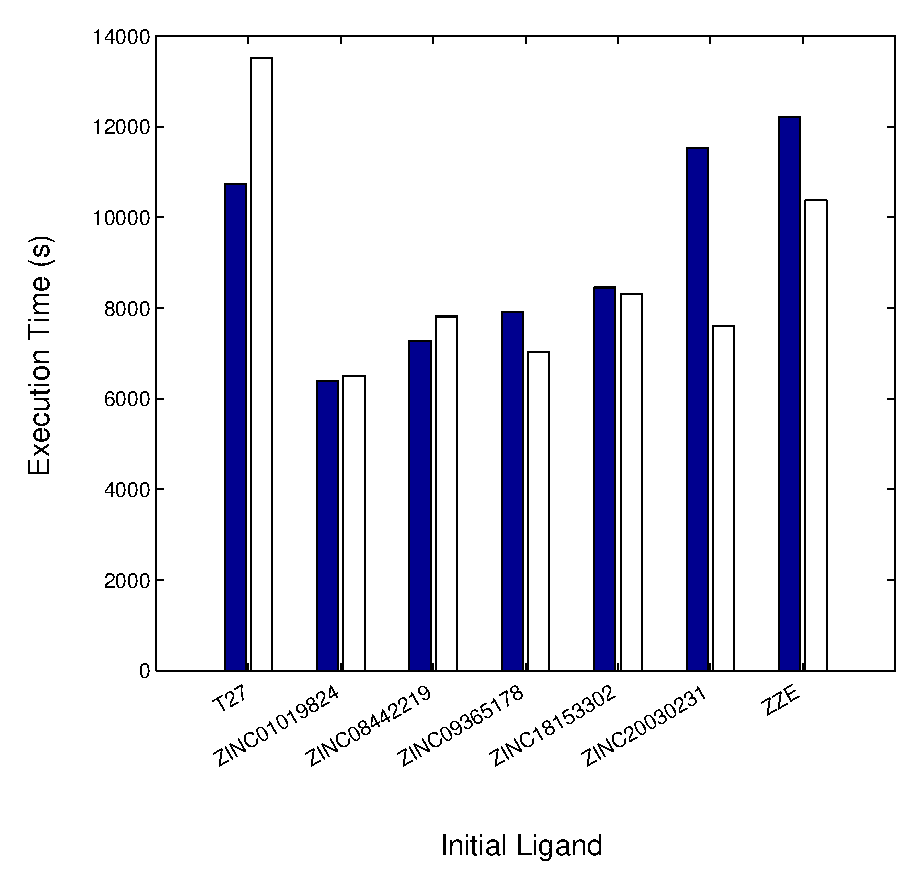
\includegraphics[width=0.31\linewidth]{Figures/Results/ExecutionTime-2ZD1.eps}
%    \label{subfig:ExecutionTime-2ZD1}
%  }
%  \subfloat[HIV PR]{
%    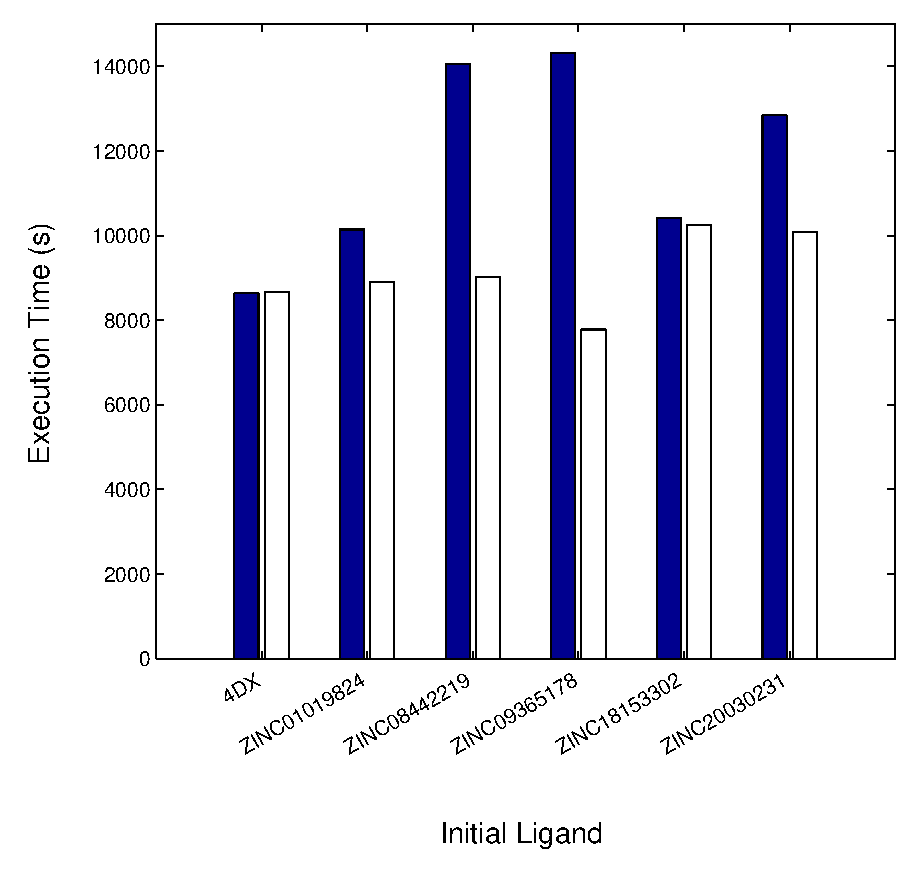
\includegraphics[width=0.31\linewidth]{Figures/Results/ExecutionTime-3KFN.eps}
%    \label{subfig:ExecutionTime-3KFN}
%  }
%  \subfloat[GSK3$\beta$]{
%    \includegraphics[width=0.31\linewidth]{Figures/Results/Speedup-1J1B.eps}
%    \label{subfig:Speedup-1J1B}
%  }
%  \subfloat[HIV RT]{
%    \includegraphics[width=0.31\linewidth]{Figures/Results/Speedup-2ZD1.eps}
%    \label{subfig:Speedup-2ZD1}
%  }
%  \subfloat[HIV PR]{
%    \includegraphics[width=0.31\linewidth]{Figures/Results/Speedup-3KFN.eps}
%    \label{subfig:Speedup-3KFN}
%  }
%  \caption{\subref{subfig:ExecutionTime-1J1B} - \subref{subfig:ExecutionTime-3KFN} Average execution times of AutoGrow and igrow. \subref{subfig:Speedup-1J1B} - \subref{subfig:Speedup-3KFN} Average speedups of igrow over AutoGrow.}
%  \label{fig:ExecutionTime-Speedup}
%\end{figure*}

\subsection{Handling Phosphorus}
igrow has built-in support for phosphorus. To examine such capability, from PDB we picked TFO, a phosphorus-containing initial ligand, as an additional test case. The input ligand file contained no PDB CONECT records. The result is shown in the supplementary materials, showing both the best generated ligand and the curves of predicted free energy and molecular weight. In contrast, AutoGrow failed to grow TFO.

%\begin{figure}[hb!]
%  \centering
%  \subfloat[The best ligand generated by igrow.]{
%    \includegraphics[width=1.0\linewidth]{Figures/Results/2ZD1-TFO-igrow.eps}
%    \label{subfig:2ZD1-TFO-igrow}
%  }
%  \subfloat[Average free energies and molecular weights of the best 5 ligands generated by igrow from TFO docking to HIV RT. Generation 0 refers to the initial ligand. Blue curve: average free energies. Red curve: average molecular weights.]{
%    \includegraphics[width=1.0\linewidth]{Figures/Results/Best5-2ZD1-TFO.eps}
%    \label{subfig:Best5-2ZD1-TFO}
%  }
%  \caption{igrow results of docking TFO to HIV RT.}
%  \label{fig:TFO}
%\end{figure}

\section{Discussions}\label{sec:discussions}
Through visualizing the generated ligands in complex of their respective receptors, we found that they are chemically valid, and we are thus of full confidence about the correctness of igrow. An example test case is demonstrated in figure \ref {fig:BestLigands}.
The best ligands generated by igrow have significantly lower molecular weights than those generated by AutoGrow, hence they are more likely to optimize into drugs.

Regarding the average free energies and molecular weights of the best 5 ligands generated by both programs, as shown in figure \ref{fig:Best5}, for most of the cases igrow displays a comparable free energy curve, while its molecular weight curve is remarkably lower than AutoGrow, and seldom exceeds 500, thanks to the guidance of Lipinski's rule of five and the `split' operator.

Regarding the execution time, as shown in figure \ref{fig:ExecutionTime}, igrow outperforms AutoGrow for 14 out of 18 test cases.
For the test case with GSK3$\beta$ as the receptor and ZINC20030231 as the initial ligand, igrow runs as much as 119\% faster than AutoGrow.
For the test case with HIV RT as the receptor and T27 as the initial ligand, although igrow requires 27\% more time, the generated ligands have lower free energies, as shown in figure \ref{fig:Best5}(g).
Averaging all the 18 test cases, in general igrow executes about 30\% faster than AutoGrow.

\section{Availability}
igrow is free and open source under Apache License 2.0. It is written in C++ and available at http://GitHub.com/HongjianLi/igrow.

\section{Conclusions}
We have developed igrow, an efficient tool for computational synthesis of potent ligands.
igrow has inherited the existing mutation and crossover operators from AutoGrow and we have invented two new genetic operators, namely split and merging.
The split operator ensures that ligands will not exceed upper bound.
The merging operator is basically a reversed operator of split which accelerates ligand growing.
igrow implements Lipinski's rule of five to ensure druggability.
The comprehensive results show that igrow outperforms AutoGrow in terms of free energy, molecular weight and execution time.

\bibliographystyle{IEEEtran}
\bibliography{../refworks}

\end{document}
